%---------------------------------------------------------------
% Preamble
%---------------------------------------------------------------
\documentclass[a4paper, 12pt]{article} 	% Document class
%% Packages

\usepackage[utf8]{inputenc}			% Input accented characters

%---------------------------------------------------------------
% Contents
%---------------------------------------------------------------
\usepackage[nottoc]{tocbibind} 		% Displays bibliography and other in the table of contents, option nottoc omits TOC from itself
\usepackage{todonotes} 					% Used for to-do lists
\usepackage{makeidx} 					% Creates an index at the end of the document
	\makeindex
\usepackage{textcomp}		  			% For the copyright symbol

%---------------------------------------------------------------
% Formatting
%---------------------------------------------------------------
\usepackage{float} 									% Placing inputs in current section
\usepackage{setspace}							% Sets spaces above/below an equation, 
												   			   % needed for \setlength in page.tex
	%\setlength{\abovedisplayskip}{1pt} % Space before equation
	%\setlength{\belowdisplayskip}{1pt}
	%\setlength\abovedisplayskip{0pt}
\usepackage{enumerate} 						 % Personalizes the enumerate style

%---------------------------------------------------------------
% Math
%---------------------------------------------------------------
%\usepackage{amssymb,amsmath,amsthm,enumitem}
\usepackage{amsmath} 						% Needed for command eqref
\usepackage{amssymb} 						% Needed for math fonts

%---------------------------------------------------------------
% Figures
%---------------------------------------------------------------
\usepackage{graphicx} 				% Needed for \includegraphics in article of slides
\usepackage[outdir=./]{epstopdf} 		% Avoids errors to input figures

%---------------------------------------------------------------
% Tables
%---------------------------------------------------------------
\usepackage{booktabs}			   % Clean tables, needed for \toprule \bottomrule
\usepackage{pdflscape}			   % To rotate landscape table page in PDF
\usepackage{longtable} 				% For long tables over pages
	\usepackage{bigstrut} 			 % Needed for the command \bigstrut

%\usepackage{siunitx}				% To align the decimal points

%---------------------------------------------------------------
% Hyperlinks and references
%---------------------------------------------------------------
\usepackage[colorlinks=true]{hyperref} 										  % Creates hyperlinks in the document, the option colorlinks=true gets rid of the awful boxes
\usepackage{xcolor}
	\definecolor{c1}{rgb}{0,0,1} 											  % Blue
	\definecolor{c2}{rgb}{0,0.3,0.9} 										% Light blue
	\definecolor{c3}{rgb}{0.3,0,0.9} 										% Red blue
	\hypersetup{
	    linkcolor={c1}, 															% Internal links
	    citecolor={c2}, 															% Citations
	    urlcolor={c3} 																% External links/urls
	}
%\usepackage{cite} % needed for cite
\usepackage[round,authoryear]{natbib} 	% For cite and abbrvnat bibliography style

%---------------------------------------------------------------
% Conditional Statements
%---------------------------------------------------------------
\usepackage{etoolbox}
	\newtoggle{commentboxes}
	\toggletrue{commentboxes}
	%\togglefalse{commentboxes}
	
%---------------------------------------------------------------
% Appendix
%---------------------------------------------------------------
\usepackage[page]{appendix}	% options: [titletoc,title,page,toc]; title adds 'Appendix' before each letter, page adds a separate title “Appendices” above the first appendix
	\renewcommand*\appendixpagename{Appendix}
	\renewcommand*\appendixtocname{Appendix}		   		  % Packages
%% Page Settings
%
%---------------------------------------------------------------
% Margins
%---------------------------------------------------------------
%\usepackage[top=2.54cm, bottom=2.54cm,left=3.17cm,right=3.17cm]{geometry} 
\usepackage[margin=1in]{geometry} 					% Sets the margins of the file

%---------------------------------------------------------------
% Indentation
%---------------------------------------------------------------
%\parindent=0cm 				 				% Sets space of first line of new text block

%---------------------------------------------------------------
% Spacing
%---------------------------------------------------------------
% Avoid excesive spacing between floating objects
\usepackage{setspace}\doublespacing
\AtBeginDocument{%
	\addtolength\abovedisplayskip{-0.2\baselineskip}%
	\addtolength\belowdisplayskip{-0.2\baselineskip}%
	%  \addtolength\abovedisplayshortskip{-0.5\baselineskip}%
	%  \addtolength\belowdisplayshortskip{-0.5\baselineskip}%
}

%---------------------------------------------------------------
% Hyphenation
%---------------------------------------------------------------
\sloppy 								 			% Tries to avoid hyphens
%\hyphenation{} 		   					   % Sets hyphenation of tolerance parameters
	%\hyphenpenalty=10000			   % Ridiculously high values force hyphenless
														 % may result in lines with very few words
	%\exhyphenpenalty=10000

%---------------------------------------------------------------
% Head and Foot
%---------------------------------------------------------------
\usepackage{fancyhdr} % Needed for head and foot options

%---------------------------------------------------------------
% Sources
%---------------------------------------------------------------
% Spacing without extra spacing for floating objects
%https://tex.stackexchange.com/questions/32918/how-can-i-decrease-spaces-between-equations

% Hyphenation
% http://www.jr-x.de/publikationen/latex/tipps/zeilenumbruch.html   		% Page settings
%% Personalized Macros
% Definitions, Equations, Table of Contents, Tables, Subcaptions, Paths, Text Fomats

%-------------------------------------------------------------------
% Variable Definitions
%-------------------------------------------------------------------
\providecommand{\tnr}{n}
\providecommand{\tnrfwd}{m}
\providecommand{\idxt}{t}
\providecommand{\idxi}{i}
\providecommand{\idxh}{h}
\providecommand{\idxs}{\idxt,\tnr}
\providecommand{\idxsfwd}{\tnr | \tnrfwd}
\providecommand{\idxsfwdt}{\idxt,\idxsfwd}
\providecommand{\idxspnl}{\idxi,\idxt}
\providecommand{\idxspnlfwd}{\idxi,{\idxt+\idxh}}
\providecommand{\idxspnllag}{\idxi,{\idxt-1}}
\providecommand{\idxspnllaglag}{\idxi,{\idxt-j}}
\providecommand{\fInst}{f_{\idxs}}
\providecommand{\yld}{y}
\providecommand{\xpc}{e}
\providecommand{\yZero}{\yld_{\idxs}}
\providecommand{\yZeroQ}{\yZero^{\Qmeasure}}
\providecommand{\yZeroP}{\yZero^{\Pmeasure}}
\providecommand{\yZeroE}{\yZero^{\xpc}}
\providecommand{\yZeroFwd}{\frate_{\idxsfwdt}}
\providecommand{\yZeroEfwd}{\yZeroFwd^{\xpc}}
\providecommand{\Pzero}{P_{\idxs}}
\providecommand{\Pzerolag}{P_{\idxt+1,\tnr-1}}
\providecommand{\srate}{i}
\providecommand{\shortrate}{\srate_{\idxt}}
\providecommand{\shortratelag}{\srate_{\idxt-1}}
\providecommand{\frate}{f}
\providecommand{\realrate}{r_{\idxs}}
\providecommand{\rateSvy}{\srate_{\idxs}^{survey}}
\providecommand{\SDF}{M_{\idxt+1}}
\providecommand{\SDFprod}{\ExpP \left[\Pi_{j=1} ^\tnr M_{\idxt+j}\right]}
\providecommand{\SDFsum}{\ExpQ \left[\exp \left(- \Sigma_{j=0} ^{\tnr-1} \srate_{\idxt+j} \right) \right]}
\providecommand{\Xvars}{X_{\idxt}}
\providecommand{\XvarsFwd}{X_{\idxt+1}}
\providecommand{\affineA}{A_{\tnr}}
\providecommand{\affineB}{B_{\tnr}}
\providecommand{\affineAfwd}{A_{\tnr + 1}}
\providecommand{\affineBfwd}{B_{\tnr + 1}}
\providecommand{\affineAQ}{\affineA^{\Qmeasure}}
\providecommand{\affineBQ}{\affineB^{\Qmeasure}}
\providecommand{\affineAP}{\affineA^{\Pmeasure}}
\providecommand{\affineBP}{\affineB^{\Pmeasure}}
\providecommand{\affineAe}{\affineA^{\xpc}}
\providecommand{\affineBe}{\affineB^{\xpc}}
\providecommand{\affineAeFwd}{A_{\idxsfwd}^{\xpc}}
\providecommand{\affineBeFwd}{B_{\idxsfwd}^{\xpc}}
\providecommand{\yLCnom}{\yld_{\idxs} ^{LC}}
\providecommand{\yLCsynt}{\widetilde{\yld}_{\idxs} ^{LC}}
\providecommand{\yUS}{y_{\idxs} ^{US}}
\providecommand{\yUSsynt}{\widetilde{\yld}_{\idxs} ^{US}}
\providecommand{\fx}{\mathit{s}}

% Math fonts
\providecommand{\Xdim}{\mathrm{K}}
\providecommand{\Ydim}{\mathrm{N}}
\providecommand{\Sdim}{\mathrm{S}}
\providecommand{\Normal}{\mathcal{N}}
\providecommand{\Pmeasure}{\mathbb{P}}
\providecommand{\Qmeasure}{\mathbb{Q}}
\providecommand{\Expec}{\mathrm{E}_{t}}
\providecommand{\ExpP}{\mathrm{E}^{\Pmeasure}_{t}}
\providecommand{\ExpQ}{\mathrm{E}^{\Qmeasure}_{t}}
\providecommand{\Svy}{S}
\providecommand{\yVec}{\mathbf{\yld}_{t}}
\providecommand{\ySVec}{\yVec^{\Svy}}
\providecommand{\Avec}{\mathbf{A}}
\providecommand{\Bvec}{\mathbf{B}}
\providecommand{\ASvec}{\mathbf{A}^{\Svy}}
\providecommand{\BSvec}{\mathbf{B}^{\Svy}}
\providecommand{\uVec}{\mathbf{u}_{t}}
\providecommand{\uSVec}{\mathbf{u}_{t}^{\Svy}}
\providecommand{\Svec}{\mathbf{\Sigma}}
\providecommand{\SyVec}{\mathbf{\Svec}_{Y}}
\providecommand{\SsVec}{\mathbf{\Svec}_{\Svy}}

% Greeks
\providecommand{\termprm}{\tau_{\idxs}}
\providecommand{\riskprice}{\lambda_{t}}
\providecommand{\lambdazero}{\lambda_{0}}
\providecommand{\lambdaone}{\lambda_{1}}
\providecommand{\fwdprm}{\rho_{\idxs}}
\providecommand{\CIPdev}{\phi_{\idxs}}
\providecommand{\deltazero}{\delta_{0}}
\providecommand{\deltaone}{\delta_{1}}
\providecommand{\error}{\nu_{t+1}}
\providecommand{\errorQ}{\error^{\Qmeasure}}
\providecommand{\errorP}{\error^{\Pmeasure}}
\providecommand{\XmuP}{\mu^{\Pmeasure}}
\providecommand{\XmuQ}{\mu^{\Qmeasure}}
\providecommand{\XSigma}{\Sigma}
\providecommand{\XPhiP}{\Phi^{\Pmeasure}}
\providecommand{\XPhiQ}{\Phi^{\Qmeasure}}
\providecommand{\betaLT}{\beta_{0}}
\providecommand{\betaST}{\beta_{1}}
\providecommand{\betaMTns}{\beta_{2}}
\providecommand{\betaMTnss}{\beta_{3}}
\providecommand{\tauNS}{\tau_{1}}
\providecommand{\tauNSS}{\tau_{2}}
\providecommand{\tnrTauNS}{\tnr/\tauNS}
\providecommand{\tnrTauNSS}{\tnr/\tauNSS}
\providecommand{\params}{\theta}
\providecommand{\Vasy}{\Omega}
\providecommand{\cmpnt}{\Psi}
\providecommand{\Jacobian}{\Gamma}
\providecommand{\Hessian}{\mathcal{H}_\params}
\providecommand{\asydstr}{\sqrt{\Ydim} \left( \widehat{\cmpnt} - \cmpnt \right) \xrightarrow[]{d} \Normal \left(0,\, \Jacobian \, \Vasy \, \Jacobian' \right)}
\providecommand{\sampleHjoint}{\frac{1}{\Ydim} \frac{\partial^{2} \ell_{\Ydim} (\widehat{\params})}{\partial \params \partial \params'}}
\providecommand{\sampleHindiv}{\frac{1}{\Ydim} \sum_{i = 1}^{\Ydim} \frac{\partial^{2} \log \mathit{f} (X_{i} | \widehat{\params})}{\partial \params \partial \params'}}

% Nelson-Siegel_Svensson
\providecommand{\loadSTnsFwd}{\exp\left(-\tnrTauNS \right)}
\providecommand{\loadSTnssFwd}{\exp\left(-\tnrTauNSS \right)}
\providecommand{\loadMTnsFwd}{\left(\tnrTauNS\right) \loadSTnsFwd}
\providecommand{\loadMTnssFwd}{\left(\tnrTauNSS\right) \loadSTnssFwd}
\providecommand{\loadSTnsZero}{\frac{1-\loadSTnsFwd}{\tnrTauNS}}
\providecommand{\loadSTnssZero}{\frac{1-\loadSTnssFwd}{\tnrTauNSS}}
\providecommand{\loadMTnsZero}{\left(\loadSTnsZero - \loadSTnsFwd \right)}
\providecommand{\loadMTnssZero}{\left( \loadSTnssZero - \loadSTnssFwd \right)}

%\providecommand{\}{}
% DELETE in a later revision
\providecommand{\Xmu}{\mu}
\providecommand{\XPhi}{\Phi}
\providecommand{\XmuStar}{\mu^{*}}
\providecommand{\XPhiStar}{\Phi^{*}}
\providecommand{\STrate}{r}
\providecommand{\rShort}{\STrate_{t}}
\providecommand{\rShortlag}{\STrate_{t-1}}
\providecommand{\ySvy}{\STrate_{\idxs}^{survey}}
\providecommand{\TPatsm}{tp_{\idxs}}

%-------------------------------------------------------------------
% Equations
%-------------------------------------------------------------------
\newcommand{\eqyLCsynt}{\yLCsynt = \yUS + \fwdprm}
\newcommand{\eqCIPdevDS}{\CIPdev = \yLCnom - \yLCsynt}
\newcommand{\eqCIPdevQ}{\CIPdev = \yLCnom - \yZeroQ}

\newcommand{\PzeroP}{\Pzero = \ExpP \left[ \SDF \Pzerolag \right]}
\newcommand{\PzeroQ}{\Pzero = \ExpQ \left[ \exp\left(- \shortrate\right) \Pzerolag \right]}

\newcommand{\eqXvarsFwdQ}{\XvarsFwd = \XmuQ + \XPhiQ \Xvars  + \XSigma \errorQ}
\newcommand{\eqshortrate}{\shortrate = \deltazero + \deltaone' \Xvars}
\newcommand{\eqyZeroP}{\yZeroP = \affineAP + \affineBP \Xvars}
\newcommand{\eqyZeroQ}{\yZeroQ = \affineAQ + \affineBQ \Xvars}
\newcommand{\eqTP}{\termprm = \yZeroQ - \yZeroP}
\newcommand{\eqXvarsFwdP}{\XvarsFwd = \XmuP + \XPhiP \Xvars  + \XSigma \errorP}
\newcommand{\eqriskprice}{\riskprice = \lambdazero + \lambdaone \Xvars}
\newcommand{\eqSDF}{\SDF = \exp\left( -\shortrate -\frac{1}{2} \riskprice' \riskprice - \riskprice' \errorP \right)}
%\newcommand{}{}

\newcommand{\eqpanelUCSV}{\tau_{\idxspnl} = \alpha_{\idxi} + \beta_{1} \sigma^{\pi}_{\idxspnl} + \beta_{2} GDP_{\idxspnl} + u_{\idxspnl}}
\newcommand{\eqpanelTPreg}{\yld_{\idxspnl} = \alpha_{\idxi} + \gamma_{1}' z^{1}_{\idxspnl} + \gamma_{2}' z^{2}_{\idxspnl} + u_{\idxspnl}}
\newcommand{\eqySvy}{\rateSvy = \frac{\widehat{\beta}_{0}}{1-\widehat{\beta}_{\srate}} + \frac{\widehat{\beta}_{{\pi}}}{1-\widehat{\beta}_{\srate}} \pi_{\idxs}^{survey} + \frac{\widehat{\beta}_{{g}}}{1-\widehat{\beta}_{\srate}} g_{\idxs}^{survey} }

\newcommand{\eqyFwd}{\yZeroFwd = \left( \tnrfwd \yld_{\idxt,\tnrfwd} - \tnr \yZero \right)/ \left( \tnrfwd - \tnr \right) }
\newcommand{\eqAeFwd}{\affineAeFwd = \left( \tnrfwd A_{\tnrfwd}^{\xpc}  - \tnr \affineAe \right)/ \left( \tnrfwd - \tnr \right) }
\newcommand{\eqBeFwd}{\affineAeFwd = \left( \tnrfwd B_{\tnrfwd}^{\xpc}  - \tnr \affineBe \right)/ \left( \tnrfwd - \tnr \right) }
\newcommand{\eqrrt}{\rateSvy = \realrate^{*} + \pi^{e}_{\idxs} = \left( \srate^{SPF survey}_{\idxs} - \pi^{SPF survey}_{\idxs} \right) + \fwdprm^{\perp} + \pi^{CE survey}_{\idxs} }


\newcommand{\eqyVecY}{\yVec = \Avec + \Bvec \Xvars + \SyVec \uVec}
\newcommand{\eqyVecS}{\ySVec = \ASvec + \BSvec \Xvars + \SsVec \uSVec}

% One shock at a time
%\newcommand{\eqpanelLP}{\yld_{\idxspnlfwd} - \yld_{\idxspnllag} = \alpha_{\idxh,\idxi} + \beta_{\idxh} \epsilon_{\idxt} + \gamma_{\idxh} \Delta \yld_{\idxspnllag} + \phi_{\idxh} \fx_{\idxspnllag}  + u_{\idxspnlfwd}}

% All shocks at once
\newcommand{\eqpanelLP}{\yld_{\idxspnlfwd} - \yld_{\idxspnllag} = \alpha_{\idxh,\idxi} + \sum^{3}_{j = 1} \beta^{j}_{\idxh} \epsilon^{j}_{\idxt} + \gamma_{\idxh} \Delta \yld_{\idxspnllag} + \eta_{\idxh} \fx_{\idxspnllag}  + u_{\idxspnlfwd}} 

\newcommand{\eqpanelLPlevels}{\yld_{\idxspnlfwd} = \alpha_{\idxh,\idxi} + \sum^{3}_{j = 1} \beta^{j}_{\idxh} \epsilon^{j}_{\idxt} + \sum^{2}_{j = 1} \gamma^{j}_{\idxh} \yld_{\idxspnllaglag} + \eta_{\idxh} \fx_{\idxspnllag}  + u_{\idxspnlfwd}} 
% \beta^{target}_{\idxh} \epsilon^{target}_{\idxt} + \beta^{path}_{\idxh} \epsilon^{path}_{\idxt} + \beta^{lsap}_{\idxh} \epsilon^{lsap}_{\idxt} 

%---------------------------------------------------------------
% Table of Contents
%---------------------------------------------------------------
% Link to ToC from section
\newcommand{\gototoc}{\vspace{-2cm} \null\hfill [\hyperlink{toc}{Go2ToC}] \newline}

% Link back to section from ToC
\newcommand{\maketoc}{
	\hypertarget{toc}{}
	\newpage
	\tableofcontents
	\vspace{2.5\bigskipamount} }

% Box with bullets for tasks to do in a section
\newenvironment{boxeditems}
	{\begin{tabular}{|p{\linewidth}|}
	\hline
	\begin{itemize}
	}
	{
	\end{itemize}
	\\ \hline
	\end{tabular} \\
	}

%---------------------------------------------------------------
% Tables: Estout Commands following Jörg Weber
%---------------------------------------------------------------
\newcommand{\sym}[1]{\rlap{#1}}

\let\estinput=\input	% define new input command to flatten the document

\newcommand{\estauto}[2]{
	\newcolumntype{C}{>{\centering\arraybackslash}X}
	\vspace{.75ex}{
%		\begin{tabularx}{1.4\textwidth}{l*{#2}C}
		\begin{tabularx}{0.95\linewidth}{l*{#2}C}
			\toprule
			\estinput{#1}
			\\ \bottomrule
			\addlinespace[.75ex]
		\end{tabularx}
	}
}

% Allow line breaks with \\ in specialcells
\newcommand{\specialcell}[2][c]{\begin{tabular}[#1]{@{}c@{}}#2\end{tabular}}

%---------------------------------------------------------------
% Subcaptions
%---------------------------------------------------------------
% Notes after figures following Jörg Weber
\newcommand{\figtext}[1]{
	\vspace{-1ex}
	\captionsetup{justification=justified,font=footnotesize}
	\caption*{#1}
%	\captionsetup{justification=raggedright,singlelinecheck=false,font=footnotesize}
%	\caption*{\hspace{6pt}\hangindent=1.5em #1}
}

\newcommand{\fignote}[1]{\figtext{\emph{Note:~}~#1}}
\newcommand{\fignotes}[1]{\figtext{\emph{Notes:~}~#1}}

% Notes after tables
\newcommand{\tabnote}[1]{
	\begin{tablenotes}[para,flushleft]
		\footnotesize \emph{Notes:~}~#1
	\end{tablenotes}
}

%---------------------------------------------------------------
% Paths
%---------------------------------------------------------------
%\newcommand*{\pathFigs}{../Figures}
%\input{pathFigs/fig1.tex}

%---------------------------------------------------------------
% Text Fomats
%---------------------------------------------------------------
%\newcommand{\txtbi}[1]{\textbf{\textit{#1}}}

%---------------------------------------------------------------
% Other
%---------------------------------------------------------------
%\newcommand\LL[1]{\multicolumn{2}{|l}{#1}}
%\newcommand\RR[1]{\multicolumn{2}{c|}{#1}}
%\newcommand\LR[1]{\multicolumn{2}{|c|}{#1}}
%\newcommand\LL[1]{\multicolumn{1}{|c}{#1}}
%\newcommand\RR[1]{\multicolumn{1}{c|}{#1}}
%\newcommand\LR[1]{\multicolumn{1}{|c|}{#1}}					   % Personalized commands
%---------------------------------------------------------------

\begin{document}
%---------------------------------------------------------------
% Title
%---------------------------------------------------------------
\title{Term Premia in Emerging Markets}% \thanks{ }}
\author{M. Pavel Solís M. 
	\thanks{Address: Wyman Park Building 544E, 3400 N. Charles Street, Baltimore, MD 21218. Email: \href{mailto:msolism1@jhu.edu}{\texttt{msolism1@jhu.edu}}.}}
\date{}
\maketitle
\vspace{-4ex}
\begin{center}
	This version: \today
\end{center}

%---------------------------------------------------------------
% Contents
%---------------------------------------------------------------
\begin{abstract}
	Bond risk premia in advanced countries is usually associated with a term premium, a compensation demanded by investors for bearing interest rate risk.
	For emerging markets, however, the two concepts are different.
	To show this, I estimate affine term structure models using a new dataset of synthetic local currency yields and survey forecasts.
	This allows me to decompose the sovereign bond yields of 15 emerging markets into an expected future short-term interest rate and a bond risk premium, which consists of a credit risk premium and a pure term premium.
	I then discuss several new insights about the dynamics of bond yields in emerging markets, including a trade-off between explicit and implicit defaults, the levels of their long-term real interest rates, the response of their term premia to U.S. quantitative easing announcements and the asymmetric effects of global factors on their yield curves.
%	addressing (which boil down to) the drivers of the BRP and the international spillovers  of the U.S. monetary policy. First, BRP is driven by global and domestic factors, the role of... being relatively larger. Second, the yield components of EMs react to US MPS asymmetrically throughout the yield curve.
% After presenting some stylized facts about the components of their yields, I show that... Finally, I document that...

%a bond risk premium, which is further disaggregated into a credit risk premium and a pure term premium.
%	the negative relationship between the two components of their bond risk premia, 
%	This decomposition leverages on synthetic local currency yields and survey data.
%	The main component of long-term yields is the expected short rate, followed by the term premium, whose size more than doubles the credit risk premium. 
%	This decomposition provides new insights into the dynamics of bond yields in emerging markets.
%First, their term premia declined in response to U.S. quantitative easing announcements.
%Second, the levels of their long-term expected real interest rates are similar to those in advanced countries.
%Finally, there is less comovement in the components of the yields of emerging markets relative to advanced countries.
%	I overcome two common concerns when analyzing these yields by using synthetic local currency yield curves to account for credit risk and survey forecasts to address the small sample problem.
%	 and their risk premia is time-varying.
%	The comovement is mainly driven by the 
%	In fact, the term premia is more globally connected than the credit risk premia and the expected short rates.
%	Further, the global component of term premia is highly linked to the U.S. term premia, whereas its idiosyncratic component is countercyclical. 
%	Second, [a recent reduction in term premia owes in part to declining inflation uncertainty among emerging markets.]
%	Finally, U.S. monetary policy shocks mainly affect component(s): [1, 2, 3].
	
	% Find the word count in the terminal: pbpaste | wc -w
	\vspace{0.5cm}
	\noindent \textit{Keywords}: Synthetic yields, term premium, credit risk, emerging markets, affine term structure models, international spillovers.
	
	\vspace{0.2cm}
	\noindent \textit{JEL Classification}: E43, F34, G12, G15, H63.
	
	\vfill
	
	\pagebreak
\end{abstract}

\section{Introduction}
\iftoggle{toclinks}{\gototoc}{} % Turn it on/off in packages.tex, command in macros.tex
\iftoggle{cboxes}{	   				  % Turn it on/off in packages.tex
	\begin{boxeditems}
		\item None.
	\end{boxeditems}}{}

U.S. monetary policy has worldwide consequences, yet the channels through which it affects the sovereign bond yields of emerging markets are not well understood. Since sovereign yields are the benchmark to price other domestic assets, the ability of emerging markets to mitigate any undesired impact from U.S. monetary policy relies on understanding those channels. 
Decomposing the yields and analyzing how the components respond is a sensible approach, but traditional two-part decompositions are not suitable for emerging market bond yields because they are assumed to be free of credit risk.

\iftoggle{fulldraft}{	% Turn it on/off in packages.tex

The main contribution of this paper is to empirically quantify the transmission channels of U.S. monetary policy to the sovereign yields of emerging markets. 
To achieve this, the paper first proposes a novel three-part decomposition of the yields that accounts for credit risk, and then asks how U.S. monetary policy transmits to those components. 
%\cite{Bernanke:2017} contends that evidence of the existence of a global financial cycle is silent about its empirical relevance.

Investors holding local currency bonds of emerging markets bear two major risks. One is the risk of not receiving the promised payments. 
Although emerging markets have increasingly borrowed in local currency over the last two decades \citep{IMFWB:2020}, they remain prone to default  \citep{ReinhartRogoff:2011,JeanneretSouissi:2016,BeersJonesWalsh:2020}.\footnote{ Before 2000, several emerging markets issued bonds at short maturities and in foreign currency. Nowadays, they mostly issue bonds with longer maturities and in local currency. Since 1996, there have been more than 30 default episodes in local currency \citep{JeanneretSouissi:2016}, including Barbados (2018), Jamaica (2013, 2010), Nicaragua (2008, 2003), Argentina (2001), Turkey (1999), Russia (1998).} 
The other is the risk that inflation erodes the real value of bond payments; the compensation for this risk is the standard term premium. Thus, compensation for credit risk addresses the risk of not receiving the promised payments, whereas the term premium compensates investors for bearing interest rate risk. 

To account for credit risk, I construct synthetic, default-free yields in local currency by essentially swapping the U.S. yield curve into a local currency one using currency derivatives. 
The yields can be seen as the borrowing rates paid by a hypothetical local currency bond issuer with no credit risk,\footnote{ Under this approach, the U.S. yield curve serves as a default-free benchmark for other countries. Although \cite{ACCS:2021} argue that U.S. sovereign default risk is not zero, it is not volatile enough to affect the results for emerging markets.} and so traditional decompositions can be applied to them. I use a standard affine term structure model augmented with survey data to obtain robust decompositions of the synthetic yields.\footnote{ \cite{Guimaraes:2014} shows that affine term structure models augmented with survey data provide robust decompositions of the U.S. and U.K. (nominal) yield curves.} Such yields have been widely used to study deviations from covered interest rate parity (CIP) but, instead of concentrating on the CIP deviations, I focus on the synthetic yields themselves.\footnote{ \cite{DuTepperVerdelhan:2018} show that persistent and systematic deviations from CIP reflect a higher regulatory burden for financial intermediaries. \cite{DuImSchreger:2018JIE} argue that they reflect differences in convenience yields in advanced economies, whereas \cite{DuSchreger:2016JoF} show that they capture a local currency credit spread for emerging markets, which is used by \cite{HofmannShimShin:2020} to explain the link between currency appreciations and the compression of the sovereign yield spreads of emerging markets.} To the best of my knowledge, this is the first application of affine term structure models to synthetic yields. 

This paper decomposes the nominal (or actual) yields of 15 emerging markets from 2000 to 2021 into three parts. The first two components come from the decomposition of the synthetic yields, namely an average expected future short rate and a term premium. The third component is the spread between the nominal and the synthetic yields, which captures the compensation for credit risk in the local currency debt of emerging markets \citep{DuSchreger:2016JoF}.\footnote{ Credit risk here is broadly defined including, for example, (selective) default risk, currency convertibility risk, regulation risk, capital controls, and jurisdiction risk, so compensation for any of these risks is considered as compensation for credit risk, even if the country does not default per se.} 
This decomposition gives reasonable estimates for the components.
Across emerging markets, the average expected short rate, the term premium and the credit risk compensation in the 10-year nominal yield represent on average 4.0, 2.2 and 0.9\%, respectively.
Credit risk is thus an important component, yet the literature on term structures of emerging market yields has not examined it systematically.\footnote{ The analysis of sovereign credit risk traditionally focuses on bonds denominated in foreign currency. For instance, \cite{HilscherNosbusch:2010} report the relevance of domestic factors to explain sovereign credit risk, while \cite{Longstaffetal:2011} document the importance of global factors. \cite{BostanciYilmaz:2020} study the connectedness of the network of sovereign credit default swaps.} By explicitly accounting for credit risk, the second component is a genuine term premium. 
I show that this term premium compensates investors for bearing inflation uncertainty, consistent with the evidence for advanced economies \citep{Wright:2011} and with inflation in emerging markets being more volatile than in advanced economies \citep{HaKoseOhnsorge:2019}. 

In addition to the three-part yield decompositions, the characterization of the transmission channels of U.S. monetary policy requires one to identify unanticipated policy decisions by the Fed. 
Following the literature \citep{Kuttner:2001,GSS:2005a,Swanson:2021}, I use intraday data around Fed's monetary policy announcements and distinguish between target, forward guidance and asset purchase surprises. 
This is by now a well-established strategy to overcome endogeneity concerns because it isolates the surprise component of monetary policy decisions.

Three main findings summarize the transmission channels of U.S. monetary policy surprises to emerging market yields.
First, the responses to target, forward guidance and asset purchase surprises are economically significant but sluggish, they amplify over the month following the surprise. This delayed response is consistent with the evidence for the U.S. and other advanced economies, which \cite{BrooksKatzLustig:2019} attribute to a portfolio rebalancing channel and slow-moving capital. 
Moreover, the effects of asset purchase surprises last longer in emerging market yields than in U.S. yields, which suggests that portfolio rebalancing involving emerging market bonds following asset purchases is slower.

Second, U.S. monetary policy transmits to emerging market yields through a yield curve channel. 
It influences not only the components of the U.S. yield curve, but the different components of the yield curves of emerging markets. 
In particular, changes in U.S. yields pass through the expected future short rate, due to what \cite{Kalemli-Ozcan:2019} calls risk spillovers, as well as through the term premium as suggested by \cite{Turner:2014} and \cite{KolasaWesolowski:2020}. 
Relatedly, the long-term yields of emerging markets are now more interconnected than short-term ones, so the global financial cycle is more relevant for the long end of their yield curves; equivalently, their monetary autonomy is stronger at the front end of their curves \citep{Obstfeld:2015}. 
In this sense, emerging markets remain vulnerable to global risks even when they borrow in local currency \citep{CarstensShin:2019}.

Third, surprises in U.S. monetary policy spill over to all yield components, so that unanticipated Fed's policy decisions lead to a reassessment of policy rate expectations and a repricing of risks in emerging markets. 
Investors expect monetary authorities in those countries to eventually follow the Fed's monetary stance rather than counteract it, given that average expected future short rates decline following target, forward guidance and asset purchase easing surprises.
In addition, Fed's unconventional monetary policies aimed at reducing the U.S. term premium, namely forward guidance and asset purchases, ultimately also decrease the term premia in emerging markets; an effect that is only detected after accounting for credit risk. 
Meanwhile, long-term credit risk compensation increases following target and forward guidance easing surprises. 
Intuitively, loose financial conditions abroad trigger a `reach-for-yield' behavior among investors \citep{HausmanWongswan:2011} that can incentivize more borrowing in emerging markets by sovereigns in local currency \citep{BigioNunoPassadore:2018} and by corporates in foreign currency\footnote{\cite{DuSchreger:2017WP} show that higher reliance on foreign currency borrowing by corporates increases sovereign default risk in emerging markets.}. 
In either case, the price of default risk (not necessarily the risk itself) increases.\footnote{In line with this, \cite{JeanneretSouissi:2016} conclude that global factors affect investors’ compensation for holding sovereign credit risk, but not the risk itself.} 
This effect could be seen as the fiscal implications in emerging markets of Fed's monetary policies, something that has so far not been discussed in the literature. 

A growing literature analyzes the spillover effects of U.S. monetary policy to the local currency sovereign bond yields of emerging markets. \cite{HausmanWongswan:2011} report significant spillovers, while \cite{BowmanLondonoSapriza:2015} compare the effects of conventional and unconventional monetary policies. The present paper is nonetheless more closely related to the work of \cite{CurcuruKaminLiRodriguez:2018}, \cite{ACDM:2019} and \cite{Albaglietal:2019}, who decompose the yields to analyze the transmission channels of such spillovers, but it differs in a number of dimensions. Most importantly, this paper explicitly accounts for the credit risk embedded in emerging market yields, and analyzes the effects of different types of monetary policy surprises identified with intraday data.\footnote{\cite{RogersScottiWright:2014} and \cite{RogersScottiWright:2018} analyze the spillovers on bond yields using surprises identified with intraday data but they focus on advanced economies. \cite{GilchristYueZakrajsek:2019} study the effects for advanced and emerging countries but for debt denominated in foreign currency.}

The rest of the paper proceeds as follows. 
Section \ref{sec:LCYCs} explains how to construct the local currency yield curves. Section \ref{sec:Methodology} presents the affine term structure model used to decompose the yields.
Section \ref{sec:Decomposition} assesses the yield decompositions.
Section \ref{sec:analysis} analyzes the U.S. monetary policy spillovers to emerging market yields.
The last section concludes.

%Theoretical explanations of why EM can default in LC: small cost to default in LC if already defaulted in FC, if external debt of firms is large don't want to default in FC. Du and Schreger, Galli
%Why it is important: risk management (simulations), portfolio allocation (high term premium), monetary policy transmission (effects on the components of yields).

}{}	% Closes \iftoggle{fulldraft}


\section{Local Currency Yield Curves} \label{sec:LCYCs}
\iftoggle{toclinks}{\gototoc}{} % Turn it on/off in packages.tex, command in macros.tex
\iftoggle{cboxes}{	   				  % Turn it on/off in packages.tex
	\begin{boxeditems}
		\item None.
	\end{boxeditems}}{}

This section explains how to construct the nominal and synthetic local currency (LC) yield curves of emerging markets, and explains that the spread between the two is a model-free measure of the compensation for credit risk. 
The next section decomposes the \textit{synthetic} yield curve into average expected future short-term interest rates and a term premium. 
The three components of the \textit{nominal} yield curve will then be used to characterize the responses of emerging market yields to U.S. monetary policy.


\iftoggle{fulldraft}{					% Turn it on/off in packages.tex

\subsection{Construction of Synthetic Yield Curves} \label{sec:YCsynt}
The main idea to construct the synthetic LC yield curves is to use the U.S. yield curve as the benchmark for all other countries and to swap it into LC by adding a foreign exchange forward premium at each maturity. 
The forward premium compensates investors for the expected depreciation of the currency.
In this paper the exchange rate is expressed in LC per U.S. dollar (USD), so a currency depreciates when the exchange rate increases.
This approach assumes frictionless financial markets; in particular, it assumes that (i) unconstrained arbitrageurs have access to U.S. and LC bonds, (ii) the derivatives contracts used to construct the forward premium have no counterparty risk, and (iii) U.S. yields are free of default risk.\footnote{ \cite{ACCS:2021} argue that U.S. sovereign default risk is not zero. Nevertheless, it is not volatile enough to affect the results in this paper.}
\cite{DuSchreger:2016JoF} show that this approach is a useful benchmark to quantify credit risk in the LC debt of emerging markets.

The zero-coupon synthetic LC yield for an \(\tnr\)-period bond at time \(\idxt\), \(\yLCsynt\), is defined as
	\begin{equation} \label{eq:nLCsynt}
	\eqyLCsynt .
\end{equation}
\noindent in which \(\yUS\) denotes the zero-coupon yield for an \(\tnr\)-period U.S. Treasury security at time \(\idxt\), and \(\fwdprm\) is the \(\tnr\)-period forward premium from USD to LC at time \(\idxt\). 
The calculation of the forward premium depends on the maturity. 
For maturities shorter than one year, the forward premium is calculated as the annualized difference between the forward and the spot exchange rates. 
For maturities equal or larger than one year, the forward premium is calculated using cross-currency swaps because outright forwards are less liquid. 
Since fixed-for-fixed cross-currency swap rates are rarely observed in the market directly, they are constructed using cross-currency basis swaps and interest rate swaps with the purpose of exchanging cash flows in the two currencies, USD and LC. 
Start by swapping fixed payments in LC into floating-rate cash flows in USD using cross-currency basis swaps (referenced to the Libor---London interbank offered rate---in USD), which are then swapped into fixed-rate cash flows in USD using interest rate swaps. Both types of swaps are liquid, marked to market and collateralized instruments, so the bilateral counterparty risk in cross-currency swaps is small.

Since the construction of synthetic yields relies on the U.S. yield curve and currency derivatives, it does not require information about the nominal yields.\footnote{ Since there is no forward premium for the USD relative to the USD, \(\yUSsynt = \yUS\).} By contrast, the nominal zero-coupon yield, \(\yLCnom\), is constructed directly from quotes of LC bonds actually traded in the market.

According to the CIP condition, the nominal (direct) and the synthetic (indirect) LC interest rates should be equal. 
Essentially, CIP implies that an issuer should be able to borrow directly or indirectly (synthetically) in LC at the same yield. 
\cite{DuTepperVerdelhan:2018} show, however, that there are persistent and systematic deviations from CIP. 
Indeed, the spread between the nominal and synthetic yields (\(\yLCnom - \yLCsynt\)) measures CIP deviations in sovereign yields.
For advanced economies, \cite{DuImSchreger:2018JIE} argue that CIP deviations measure the difference in the convenience yield of U.S. Treasuries relative to that of the sovereign bonds of other advanced economies.
By contrast, \cite{DuSchreger:2016JoF} point out that CIP deviations have a different interpretation for emerging markets. 

The nominal-synthetic spread is a model-free measure of the compensation for credit risk in the LC yields of emerging markets. 
Whereas the nominal yields of advanced economies are usually considered free of credit risk, the nominal yields of emerging markets include a credit risk compensation given the possibility of default \citep{DuSchreger:2016JoF,DuSchreger:2017WP}. 
Since credit risk in the components of the synthetic yields (equation (\ref{eq:nLCsynt})) is small, a synthetic yield in emerging markets can be seen as the borrowing rate paid by a hypothetical issuer in LC with no credit risk. 
\cite{DuSchreger:2016JoF} show that the nominal-synthetic spread is highly correlated with the rates of sovereign credit default swaps (CDS)---financial derivatives aimed to protect investors against default by a bond issuer. 
However, while CDS are suitable for studying the sovereign risk in bonds denominated in foreign currency \cite[see, for example,][]{Longstaffetal:2011}, \cite{DuSchreger:2016JoF} argue that the nominal-synthetic spread adequately measures credit risk on LC debt. 
On this regard, according to the International Swaps and Derivatives Association (ISDA), LC bonds governed under domestic law do not trigger CDS payouts.\footnote{ See the ISDA credit derivatives physical settlement matrix.} 
Moreover, a credit event for a CDS contract is not always clearly defined. 
Section \ref{sec:CRC} discusses the interpretation of the nominal-synthetic spread in more detail.


\subsection{Construction of Nominal Yield Curves} \label{sec:YCnom}
\iftoggle{toclinks}{\gototoc}{} % Turn it on/off in packages.tex, command in macros.tex

For each country, the nominal yield curve \(\yLCnom\) is a continuously-compounded zero-coupon curve. 
Its construction uses the Bloomberg Fair Value (BFV) curves for all but two countries. 
These curves report coupon-equivalent par yields, which I convert into continuously-compounded yields to obtain implied zero-coupon curves \citep[see][]{GSW:2007}.\footnote{As a robustness check, I estimate the nominal yield curves from actual prices for some of the countries in the sample using the Nelson--Siegel model. They closely follow the curves reported by Bloomberg.} 
For Brazil and Israel, Bloomberg does not provide BFV curves but zero-coupon yields with coupon-equivalent compounding, known as IYC curves, which I also convert into continuously-compounded yields.\footnote{ For some emerging markets, Bloomberg reports both BFV and IYC curves. BFV curves are preferred for several reasons: their history is longer, IYC curves are not available for advanced economies---the benchmark for some of the results reported later---and, compared to the BFV curves, the short end of the IYC curves seems disconnected from the rest of the curve at some dates for a few countries.} 


\subsection{Yield Curve Data}
\iftoggle{toclinks}{\gototoc}{} % Turn it on/off in packages.tex, command in macros.tex

Nominal and synthetic yield curves are constructed for the 15 emerging markets originally studied by \cite{DuSchreger:2016JoF} and, to compare the results, for the 10 advanced economies considered by \cite{DuImSchreger:2018JIE}.\footnote{ Emerging markets: Brazil, Colombia, Hungary, Indonesia, Israel, Korea, Malaysia, Mexico, Peru, the Philippines, Poland, Russia, South Africa, Thailand, Turkey. Advanced economies: Australia, Canada, Denmark, Germany (based on the euro), Japan, Norway, New Zealand, Sweden, Switzerland, the U.K.} 
All emerging markets in the sample, except Malaysia, have adopted an inflation targeting regime,\footnote{ Nevertheless, Malaysia has several characteristics that are aligned with an inflation targeting regime. Some countries adopted inflation targeting during the sample period: Hungary in June 2001, the Philippines in January 2002, Indonesia in July 2005, Turkey in January 2006 and Russia in 2014; Hungary and Poland were accepted to join the European Union in April 2003.} which supports the application of affine term structure models to the yields of these countries. 

The data for nominal and synthetic yields are available daily. 
The sample starts in January 2000 and ends in July 2021. The starting dates, however, vary by country.
All the yields for advanced economies start no later than September 2001.
The sample sizes for emerging markets are generally smaller.
The nominal yields of 9 and the synthetic yields of 7 emerging markets start before March 2004; both types of yields for the rest of the countries start no later than June 2007.
% Nominal before March 2004: HUF, IDR, KRW, MXN, MYR, PHP, PLN, THB, ZAR.
% Synthetic before March 2004: HUF, IDR, KRW, MXN, PHP, PLN, ZAR.
There are thus at least 10 years of data for all of the countries in the sample.\footnote{ For Turkey, the nominal yields with a maturity of up to 10 years start on June 2010, although its synthetic yields start on May 2005. For Russia, data on both types of yields start in 2007 but due to low liquidity at the beginning of the sample, here it starts in August 2009.}
In principle, this is a reasonable time period for the estimation of the affine term structure model presented in section \ref{sec:ATSM}, but in practice there may be too few interest rate cycles per country.
To address this small sample problem, the model is subsequently augmented with data from surveys of professional forecasters, as discussed in section \ref{sec:Estimation}. 

The yields have maturities of 3 and 6 months, and 1 through 10 years, ranging from a minimum of nine to a maximum of twelve maturities per country.\footnote{ All countries have data for maturities from 3 months to 5 years and for 10 years. All countries except Brazil have data for the 7-year maturity. Data for 6, 8 and 9 years vary per country.} 
The maximum maturity considered for the analysis is 10 years because bonds and swaps with larger maturities have less history and are less liquid, especially for emerging markets who do not issue longer-term bonds as often as advanced economies.

The construction of LC synthetic yield curves involves data from the U.S. yield curve and the forward premium for different maturities, as explained in section \ref{sec:YCsynt}. 
Data for the U.S. zero-coupon yield curve come from two sources. 
For maturities of 1 through 10 years, the yields come from the dataset constructed by \cite{GSW:2007}, who only consider Treasury securities with coupons. 
Since Treasury securities with less than one year to maturity behave differently \citep{Duffee:2010}---partly because they are less actively traded than longer-maturity ones---the 3- and 6-month yields come from the Federal Reserve's H.15 database because they are robust at the short end of the curve.\footnote{ The 3- and 6-month yields implied by the fitted model of \cite{GSW:2007} are highly correlated with the H.15 yields (0.9985 and 0.9995) but are on average (16 and 10 basis points) higher since 1983.} 
% CRSP data monthly and daily data fixed-rate and risk-free series are very close to each other once they are annualized. The `biggest' differences are in the 1-month interest rate and before 1980.

The data to compute the forward premium also come from two sources. 
For maturities of less than one year, I use data on the spot exchange rate along with 3- and 6-month forwards from Bloomberg for all countries but Korea, the Philippines and Thailand, for which the data come from Datastream. 
To construct the cross-currency swap rates, I use data on cross-currency basis swaps and interest rate swaps for each available maturity from 1 through 10 years. 
The data for the swap curves come from Bloomberg.\footnote{Deliverable and non-deliverable cross-currency swaps are used as well as tenor basis swaps. A spreadsheet with the tickers used in the construction of the forward premia and the estimation of the nominal yield curves is available upon request. The file consolidates and expands (with tenors and tickers) similar files kindly posted online in Wenxin Du and Jesse Schreger's websites.}

Table \ref{tab:yldcrvstats} reports descriptive statistics for different tenors of the nominal and synthetic yield curves for the emerging markets and advanced economies in the sample. 
The yield curves exhibit standard properties such as an upward slope. 
At the same time, the table provides information on how the curves of emerging markets differ from those of advanced economies. 
For instance, the level and the volatility (measured by the standard deviation) of their curves are larger than those of advanced economies. 
Also, the short end of their curves is more volatile than the long end, particularly so for the synthetic curve.
Lastly, the spread between the nominal and the synthetic yields suggests that the credit risk compensation is on average positive. 

\documentclass[a4paper,12pt]{article}
\usepackage[labelsep=period,labelfont=bf]{caption}
\usepackage{multirow}
\usepackage{booktabs}
\usepackage{threeparttable}
\usepackage{pdflscape}
\usepackage{tabularx}
%\usepackage[margin=1in]{geometry}
%%% Personalized Macros
% Definitions, Equations, Table of Contents, Tables, Subcaptions, Paths, Text Fomats

%-------------------------------------------------------------------
% Variable Definitions
%-------------------------------------------------------------------
\providecommand{\tnr}{n}
\providecommand{\tnrfwd}{m}
\providecommand{\idxt}{t}
\providecommand{\idxi}{i}
\providecommand{\idxh}{h}
\providecommand{\idxs}{\idxt,\tnr}
\providecommand{\idxsfwd}{\tnr | \tnrfwd}
\providecommand{\idxsfwdt}{\idxt,\idxsfwd}
\providecommand{\idxspnl}{\idxi,\idxt}
\providecommand{\idxspnlfwd}{\idxi,{\idxt+\idxh}}
\providecommand{\idxspnllag}{\idxi,{\idxt-1}}
\providecommand{\idxspnllaglag}{\idxi,{\idxt-j}}
\providecommand{\fInst}{f_{\idxs}}
\providecommand{\yld}{y}
\providecommand{\xpc}{e}
\providecommand{\yZero}{\yld_{\idxs}}
\providecommand{\yZeroQ}{\yZero^{\Qmeasure}}
\providecommand{\yZeroP}{\yZero^{\Pmeasure}}
\providecommand{\yZeroE}{\yZero^{\xpc}}
\providecommand{\yZeroFwd}{\frate_{\idxsfwdt}}
\providecommand{\yZeroEfwd}{\yZeroFwd^{\xpc}}
\providecommand{\Pzero}{P_{\idxs}}
\providecommand{\Pzerolag}{P_{\idxt+1,\tnr-1}}
\providecommand{\srate}{i}
\providecommand{\shortrate}{\srate_{\idxt}}
\providecommand{\shortratelag}{\srate_{\idxt-1}}
\providecommand{\frate}{f}
\providecommand{\realrate}{r_{\idxs}}
\providecommand{\rateSvy}{\srate_{\idxs}^{survey}}
\providecommand{\SDF}{M_{\idxt+1}}
\providecommand{\SDFprod}{\ExpP \left[\Pi_{j=1} ^\tnr M_{\idxt+j}\right]}
\providecommand{\SDFsum}{\ExpQ \left[\exp \left(- \Sigma_{j=0} ^{\tnr-1} \srate_{\idxt+j} \right) \right]}
\providecommand{\Xvars}{X_{\idxt}}
\providecommand{\XvarsFwd}{X_{\idxt+1}}
\providecommand{\affineA}{A_{\tnr}}
\providecommand{\affineB}{B_{\tnr}}
\providecommand{\affineAfwd}{A_{\tnr + 1}}
\providecommand{\affineBfwd}{B_{\tnr + 1}}
\providecommand{\affineAQ}{\affineA^{\Qmeasure}}
\providecommand{\affineBQ}{\affineB^{\Qmeasure}}
\providecommand{\affineAP}{\affineA^{\Pmeasure}}
\providecommand{\affineBP}{\affineB^{\Pmeasure}}
\providecommand{\affineAe}{\affineA^{\xpc}}
\providecommand{\affineBe}{\affineB^{\xpc}}
\providecommand{\affineAeFwd}{A_{\idxsfwd}^{\xpc}}
\providecommand{\affineBeFwd}{B_{\idxsfwd}^{\xpc}}
\providecommand{\yLCnom}{\yld_{\idxs} ^{LC}}
\providecommand{\yLCsynt}{\widetilde{\yld}_{\idxs} ^{LC}}
\providecommand{\yUS}{y_{\idxs} ^{US}}
\providecommand{\yUSsynt}{\widetilde{\yld}_{\idxs} ^{US}}
\providecommand{\fx}{\mathit{s}}

% Math fonts
\providecommand{\Xdim}{\mathrm{K}}
\providecommand{\Ydim}{\mathrm{N}}
\providecommand{\Sdim}{\mathrm{S}}
\providecommand{\Normal}{\mathcal{N}}
\providecommand{\Pmeasure}{\mathbb{P}}
\providecommand{\Qmeasure}{\mathbb{Q}}
\providecommand{\Expec}{\mathrm{E}_{t}}
\providecommand{\ExpP}{\mathrm{E}^{\Pmeasure}_{t}}
\providecommand{\ExpQ}{\mathrm{E}^{\Qmeasure}_{t}}
\providecommand{\Svy}{S}
\providecommand{\yVec}{\mathbf{\yld}_{t}}
\providecommand{\ySVec}{\yVec^{\Svy}}
\providecommand{\Avec}{\mathbf{A}}
\providecommand{\Bvec}{\mathbf{B}}
\providecommand{\ASvec}{\mathbf{A}^{\Svy}}
\providecommand{\BSvec}{\mathbf{B}^{\Svy}}
\providecommand{\uVec}{\mathbf{u}_{t}}
\providecommand{\uSVec}{\mathbf{u}_{t}^{\Svy}}
\providecommand{\Svec}{\mathbf{\Sigma}}
\providecommand{\SyVec}{\mathbf{\Svec}_{Y}}
\providecommand{\SsVec}{\mathbf{\Svec}_{\Svy}}

% Greeks
\providecommand{\termprm}{\tau_{\idxs}}
\providecommand{\riskprice}{\lambda_{t}}
\providecommand{\lambdazero}{\lambda_{0}}
\providecommand{\lambdaone}{\lambda_{1}}
\providecommand{\fwdprm}{\rho_{\idxs}}
\providecommand{\CIPdev}{\phi_{\idxs}}
\providecommand{\deltazero}{\delta_{0}}
\providecommand{\deltaone}{\delta_{1}}
\providecommand{\error}{\nu_{t+1}}
\providecommand{\errorQ}{\error^{\Qmeasure}}
\providecommand{\errorP}{\error^{\Pmeasure}}
\providecommand{\XmuP}{\mu^{\Pmeasure}}
\providecommand{\XmuQ}{\mu^{\Qmeasure}}
\providecommand{\XSigma}{\Sigma}
\providecommand{\XPhiP}{\Phi^{\Pmeasure}}
\providecommand{\XPhiQ}{\Phi^{\Qmeasure}}
\providecommand{\betaLT}{\beta_{0}}
\providecommand{\betaST}{\beta_{1}}
\providecommand{\betaMTns}{\beta_{2}}
\providecommand{\betaMTnss}{\beta_{3}}
\providecommand{\tauNS}{\tau_{1}}
\providecommand{\tauNSS}{\tau_{2}}
\providecommand{\tnrTauNS}{\tnr/\tauNS}
\providecommand{\tnrTauNSS}{\tnr/\tauNSS}
\providecommand{\params}{\theta}
\providecommand{\Vasy}{\Omega}
\providecommand{\cmpnt}{\Psi}
\providecommand{\Jacobian}{\Gamma}
\providecommand{\Hessian}{\mathcal{H}_\params}
\providecommand{\asydstr}{\sqrt{\Ydim} \left( \widehat{\cmpnt} - \cmpnt \right) \xrightarrow[]{d} \Normal \left(0,\, \Jacobian \, \Vasy \, \Jacobian' \right)}
\providecommand{\sampleHjoint}{\frac{1}{\Ydim} \frac{\partial^{2} \ell_{\Ydim} (\widehat{\params})}{\partial \params \partial \params'}}
\providecommand{\sampleHindiv}{\frac{1}{\Ydim} \sum_{i = 1}^{\Ydim} \frac{\partial^{2} \log \mathit{f} (X_{i} | \widehat{\params})}{\partial \params \partial \params'}}

% Nelson-Siegel_Svensson
\providecommand{\loadSTnsFwd}{\exp\left(-\tnrTauNS \right)}
\providecommand{\loadSTnssFwd}{\exp\left(-\tnrTauNSS \right)}
\providecommand{\loadMTnsFwd}{\left(\tnrTauNS\right) \loadSTnsFwd}
\providecommand{\loadMTnssFwd}{\left(\tnrTauNSS\right) \loadSTnssFwd}
\providecommand{\loadSTnsZero}{\frac{1-\loadSTnsFwd}{\tnrTauNS}}
\providecommand{\loadSTnssZero}{\frac{1-\loadSTnssFwd}{\tnrTauNSS}}
\providecommand{\loadMTnsZero}{\left(\loadSTnsZero - \loadSTnsFwd \right)}
\providecommand{\loadMTnssZero}{\left( \loadSTnssZero - \loadSTnssFwd \right)}

%\providecommand{\}{}
% DELETE in a later revision
\providecommand{\Xmu}{\mu}
\providecommand{\XPhi}{\Phi}
\providecommand{\XmuStar}{\mu^{*}}
\providecommand{\XPhiStar}{\Phi^{*}}
\providecommand{\STrate}{r}
\providecommand{\rShort}{\STrate_{t}}
\providecommand{\rShortlag}{\STrate_{t-1}}
\providecommand{\ySvy}{\STrate_{\idxs}^{survey}}
\providecommand{\TPatsm}{tp_{\idxs}}

%-------------------------------------------------------------------
% Equations
%-------------------------------------------------------------------
\newcommand{\eqyLCsynt}{\yLCsynt = \yUS + \fwdprm}
\newcommand{\eqCIPdevDS}{\CIPdev = \yLCnom - \yLCsynt}
\newcommand{\eqCIPdevQ}{\CIPdev = \yLCnom - \yZeroQ}

\newcommand{\PzeroP}{\Pzero = \ExpP \left[ \SDF \Pzerolag \right]}
\newcommand{\PzeroQ}{\Pzero = \ExpQ \left[ \exp\left(- \shortrate\right) \Pzerolag \right]}

\newcommand{\eqXvarsFwdQ}{\XvarsFwd = \XmuQ + \XPhiQ \Xvars  + \XSigma \errorQ}
\newcommand{\eqshortrate}{\shortrate = \deltazero + \deltaone' \Xvars}
\newcommand{\eqyZeroP}{\yZeroP = \affineAP + \affineBP \Xvars}
\newcommand{\eqyZeroQ}{\yZeroQ = \affineAQ + \affineBQ \Xvars}
\newcommand{\eqTP}{\termprm = \yZeroQ - \yZeroP}
\newcommand{\eqXvarsFwdP}{\XvarsFwd = \XmuP + \XPhiP \Xvars  + \XSigma \errorP}
\newcommand{\eqriskprice}{\riskprice = \lambdazero + \lambdaone \Xvars}
\newcommand{\eqSDF}{\SDF = \exp\left( -\shortrate -\frac{1}{2} \riskprice' \riskprice - \riskprice' \errorP \right)}
%\newcommand{}{}

\newcommand{\eqpanelUCSV}{\tau_{\idxspnl} = \alpha_{\idxi} + \beta_{1} \sigma^{\pi}_{\idxspnl} + \beta_{2} GDP_{\idxspnl} + u_{\idxspnl}}
\newcommand{\eqpanelTPreg}{\yld_{\idxspnl} = \alpha_{\idxi} + \gamma_{1}' z^{1}_{\idxspnl} + \gamma_{2}' z^{2}_{\idxspnl} + u_{\idxspnl}}
\newcommand{\eqySvy}{\rateSvy = \frac{\widehat{\beta}_{0}}{1-\widehat{\beta}_{\srate}} + \frac{\widehat{\beta}_{{\pi}}}{1-\widehat{\beta}_{\srate}} \pi_{\idxs}^{survey} + \frac{\widehat{\beta}_{{g}}}{1-\widehat{\beta}_{\srate}} g_{\idxs}^{survey} }

\newcommand{\eqyFwd}{\yZeroFwd = \left( \tnrfwd \yld_{\idxt,\tnrfwd} - \tnr \yZero \right)/ \left( \tnrfwd - \tnr \right) }
\newcommand{\eqAeFwd}{\affineAeFwd = \left( \tnrfwd A_{\tnrfwd}^{\xpc}  - \tnr \affineAe \right)/ \left( \tnrfwd - \tnr \right) }
\newcommand{\eqBeFwd}{\affineAeFwd = \left( \tnrfwd B_{\tnrfwd}^{\xpc}  - \tnr \affineBe \right)/ \left( \tnrfwd - \tnr \right) }
\newcommand{\eqrrt}{\rateSvy = \realrate^{*} + \pi^{e}_{\idxs} = \left( \srate^{SPF survey}_{\idxs} - \pi^{SPF survey}_{\idxs} \right) + \fwdprm^{\perp} + \pi^{CE survey}_{\idxs} }


\newcommand{\eqyVecY}{\yVec = \Avec + \Bvec \Xvars + \SyVec \uVec}
\newcommand{\eqyVecS}{\ySVec = \ASvec + \BSvec \Xvars + \SsVec \uSVec}

% One shock at a time
%\newcommand{\eqpanelLP}{\yld_{\idxspnlfwd} - \yld_{\idxspnllag} = \alpha_{\idxh,\idxi} + \beta_{\idxh} \epsilon_{\idxt} + \gamma_{\idxh} \Delta \yld_{\idxspnllag} + \phi_{\idxh} \fx_{\idxspnllag}  + u_{\idxspnlfwd}}

% All shocks at once
\newcommand{\eqpanelLP}{\yld_{\idxspnlfwd} - \yld_{\idxspnllag} = \alpha_{\idxh,\idxi} + \sum^{3}_{j = 1} \beta^{j}_{\idxh} \epsilon^{j}_{\idxt} + \gamma_{\idxh} \Delta \yld_{\idxspnllag} + \eta_{\idxh} \fx_{\idxspnllag}  + u_{\idxspnlfwd}} 

\newcommand{\eqpanelLPlevels}{\yld_{\idxspnlfwd} = \alpha_{\idxh,\idxi} + \sum^{3}_{j = 1} \beta^{j}_{\idxh} \epsilon^{j}_{\idxt} + \sum^{2}_{j = 1} \gamma^{j}_{\idxh} \yld_{\idxspnllaglag} + \eta_{\idxh} \fx_{\idxspnllag}  + u_{\idxspnlfwd}} 
% \beta^{target}_{\idxh} \epsilon^{target}_{\idxt} + \beta^{path}_{\idxh} \epsilon^{path}_{\idxt} + \beta^{lsap}_{\idxh} \epsilon^{lsap}_{\idxt} 

%---------------------------------------------------------------
% Table of Contents
%---------------------------------------------------------------
% Link to ToC from section
\newcommand{\gototoc}{\vspace{-2cm} \null\hfill [\hyperlink{toc}{Go2ToC}] \newline}

% Link back to section from ToC
\newcommand{\maketoc}{
	\hypertarget{toc}{}
	\newpage
	\tableofcontents
	\vspace{2.5\bigskipamount} }

% Box with bullets for tasks to do in a section
\newenvironment{boxeditems}
	{\begin{tabular}{|p{\linewidth}|}
	\hline
	\begin{itemize}
	}
	{
	\end{itemize}
	\\ \hline
	\end{tabular} \\
	}

%---------------------------------------------------------------
% Tables: Estout Commands following Jörg Weber
%---------------------------------------------------------------
\newcommand{\sym}[1]{\rlap{#1}}

\let\estinput=\input	% define new input command to flatten the document

\newcommand{\estauto}[2]{
	\newcolumntype{C}{>{\centering\arraybackslash}X}
	\vspace{.75ex}{
%		\begin{tabularx}{1.4\textwidth}{l*{#2}C}
		\begin{tabularx}{0.95\linewidth}{l*{#2}C}
			\toprule
			\estinput{#1}
			\\ \bottomrule
			\addlinespace[.75ex]
		\end{tabularx}
	}
}

% Allow line breaks with \\ in specialcells
\newcommand{\specialcell}[2][c]{\begin{tabular}[#1]{@{}c@{}}#2\end{tabular}}

%---------------------------------------------------------------
% Subcaptions
%---------------------------------------------------------------
% Notes after figures following Jörg Weber
\newcommand{\figtext}[1]{
	\vspace{-1ex}
	\captionsetup{justification=justified,font=footnotesize}
	\caption*{#1}
%	\captionsetup{justification=raggedright,singlelinecheck=false,font=footnotesize}
%	\caption*{\hspace{6pt}\hangindent=1.5em #1}
}

\newcommand{\fignote}[1]{\figtext{\emph{Note:~}~#1}}
\newcommand{\fignotes}[1]{\figtext{\emph{Notes:~}~#1}}

% Notes after tables
\newcommand{\tabnote}[1]{
	\begin{tablenotes}[para,flushleft]
		\footnotesize \emph{Notes:~}~#1
	\end{tablenotes}
}

%---------------------------------------------------------------
% Paths
%---------------------------------------------------------------
%\newcommand*{\pathFigs}{../Figures}
%\input{pathFigs/fig1.tex}

%---------------------------------------------------------------
% Text Fomats
%---------------------------------------------------------------
%\newcommand{\txtbi}[1]{\textbf{\textit{#1}}}

%---------------------------------------------------------------
% Other
%---------------------------------------------------------------
%\newcommand\LL[1]{\multicolumn{2}{|l}{#1}}
%\newcommand\RR[1]{\multicolumn{2}{c|}{#1}}
%\newcommand\LR[1]{\multicolumn{2}{|c|}{#1}}
%\newcommand\LL[1]{\multicolumn{1}{|c}{#1}}
%\newcommand\RR[1]{\multicolumn{1}{c|}{#1}}
%\newcommand\LR[1]{\multicolumn{1}{|c|}{#1}}

\begin{document}
	\begin{normalsize}
%		\begin{landscape}
			\begin{table}
				\begin{center}
					\caption{Descriptive Statistics of Yield Curves} \label{tab:yldcrvstats}
					\begin{threeparttable}
						\estauto{../Tables/f_yldcrvstats.tex}{7}
						\tabnote{This table reports the average, the standard deviation, the minimum and the maximum values using end-of-month data for different tenors of the nominal and synthetic yields of the emerging markets and advanced countries in the sample.  All figures are expressed in annualized percentage points.}
					\end{threeparttable}
				\end{center}
			\end{table}
%		\end{landscape}
	\end{normalsize}
\end{document}


\subsubsection{Timing}
The parameters of the affine term structure models are estimated using end-of-month data, as explained in section \ref{sec:Estimation}. 
Since the U.S. yield curve is the benchmark to construct the synthetic yield curves, the end-of-month dates are the last business days of each month according to the U.S. calendar.

Getting the timing right is key to adequately measure the responses of emerging market yields to surprises in Fed's policy decisions.
The analysis of monetary policy spillovers in section \ref{sec:LPs} uses daily changes in nominal and synthetic yields. 
Since the closing prices in non-Western Hemisphere countries happen before the Fed's monetary policy announcements, their nominal yields are shifted one day back so that their daily changes adequately capture surprises in the announcements. 
The credit risk compensation for those countries is calculated using the shifted nominal yields.

%Fed announcements at 14 hours NY time.
%Nominal LC yield curves pull at 16 hours NY time.
%Libor is announced at 11:45 hours London time.
%To get the time right, \(ysyntLC_t = yUS_t + rho_{t+1}\)

}{}	% Closes \iftoggle{fulldraft}


\section{Methodology} \label{sec:Methodology}
\iftoggle{toclinks}{\gototoc}{} % Turn it on/off in packages.tex, command in macros.tex
\iftoggle{cboxes}{	   				  % Turn it on/off in packages.tex
	\begin{boxeditems}
		\item None.
	\end{boxeditems}}{}

This section describes the affine term structure model used to decompose the yield curve of each country in the sample, and discusses the difficulties in estimating the parameters of the model. 
It then explains how survey data help in the estimation. 
Among the many applications of the decomposition, section \ref{sec:analysis} exploits it to analyze the transmission channels of U.S. monetary policy to the yields of emerging markets. 

\iftoggle{fulldraft}{					% Turn it on/off in packages.tex

\subsection{Affine Term Structure Model} \label{sec:ATSM}
Let \(\Pzero\) be the price at time \(\idxt\) of a zero-coupon \textit{risk-free} bond with maturity \(\tnr\). The continuously compounded yield on that bond is then \(\yZero = - \ln \Pzero/\tnr\). In particular, the one-period continuously compounded risk-free rate is \(\shortrate = \yld_{\idxt,1} = - \ln P_{t,1}\).

If there is no arbitrage, there exists a strictly positive stochastic discount factor that prices all nominal bonds. 
Let \(\SDF\) be the nominal stochastic discount factor. 
Accordingly, the bond price today is recursively defined as follows
	\begin{equation} \label{eq:nPzeroP}
	\PzeroP ,
\end{equation}
\noindent in which \(\ExpP [\cdot]\) denotes the conditional expectation at time \(\idxt\) taken using the actual or physical probability measure, \(\Pmeasure\), that generates the data. 
The existence of the stochastic discount factor also implies that there exists a theoretical risk-neutral or risk-adjusted pricing measure \(\Qmeasure\)---different from the \(\Pmeasure\) measure---that is defined as follows %\footnote{ Since the price at maturity of a zero-coupon bond is \(1\), recursive substitution of equations (\ref{eq:nPzeroP}) and (\ref{eq:nPzeroQ}) implies that \(\Pzero = \SDFprod = \SDFsum \).} % today's price equals the conditional expectation of the product of SDFs over the life of the bond,
	\begin{equation} \label{eq:nPzeroQ}
	\Pzero = \ExpQ \left[ \exp\left(- \shortrate\right) \Pzerolag \right],
\end{equation}
\noindent in which \(\ExpQ [\cdot]\) also denotes conditional expectation but taken under the \(\Qmeasure\)  measure.

A discrete-time affine term structure model assumes that the dynamics of a \(\Xdim \times 1\) vector of unobserved pricing factors or state variables, \(\Xvars\), follow a first-order vector autoregression, VAR(1), under the risk-neutral measure \(\Qmeasure\)
	\begin{equation} \label{eq:nXvarsQ}
	\XvarsFwd = \XmuQ + \XPhiQ \Xvars  + \XSigma \errorQ.
\end{equation}
\noindent in which \(\XmuQ\) is a \(\Xdim \times 1\) vector and \(\XPhiQ\) is a \(\Xdim \times \Xdim\) transition matrix, \(\XSigma\) is a \(\Xdim \times \Xdim\) lower triangular matrix with positive diagonal elements, and \(\errorQ\) is a \(\Xdim \times 1\) independent and identically distributed, normal vector with zero mean and covariance equal to the identity matrix conditional on the pricing factors, that is \(\error^{\Qmeasure} | \Xvars \sim \Normal_{\Xdim} \left(0,I\right)\). 

The pricing factors drive the dynamics of the one-period interest rate as follows 
	\begin{equation} \label{eq:nShortRate}
	\shortrate = \deltazero + \deltaone' \Xvars ,
\end{equation}
\noindent in which \(\deltazero\) is a scalar and \(\deltaone\) is a \(\Xdim \times 1\) vector of parameters.

These assumptions imply that the bond price is an exponentially affine function of the pricing factors
	\input{../Equations/uPaffine}
\noindent such that the corresponding continuously compounded yield of the bond is an affine function of those factors
	\begin{equation} \label{eq:nYaffineQ}
	\yZeroQ = - \frac{\affineA}{\tnr} - \frac{\affineB}{\tnr} \Xvars = \affineA^{\Qmeasure} + \affineB^{\Qmeasure} \Xvars,
\end{equation}
\noindent in which \(\affineAQ = - \frac{1}{\tnr} \affineA\), \(\affineBQ = - \frac{1}{\tnr} \affineB\), where in turn the scalar \(\affineA = \mathcal{A}(\deltazero, \deltaone, \XmuQ, \XPhiQ, \XSigma, \tnr)\) \!and the \(1 \times \Xdim\) vector \(\affineB = \mathcal{B}(\deltaone, \XPhiQ, \tnr)\) are loadings that satisfy the recursive equations
	\begin{equation} \label{eq:nAffineA}
	\affineAfwd = - \deltazero + \affineA + \affineB' \XmuQ + \frac{1}{2} \affineB' \XSigma \XSigma' \affineB , \quad A_{0} = 0 ,
\end{equation}
	\vspace{-.7cm}
	\begin{equation} \label{eq:nAffineB}
	\affineBfwd = - \deltaone + \XPhiQ{'} \affineB , \quad B_{0} = 0 .
\end{equation}
The yields \(\yZeroQ\) are the model's fitted yields, which means that the risk-neutral measure \(\Qmeasure\) is sufficient for pricing bonds. 
However, to be able to decompose the yields into an average expected future short-term interest rate and a term premium, the model needs to specify the dynamics for the market prices of risk, which control the transformation between the \(\Qmeasure\) and \(\Pmeasure\) measures. 
In this sense, the stochastic discount factor is assumed to be conditionally lognormal
\begin{equation} \label{eq:nSDF}
	\SDF = \exp\left( -\rShort -\frac{1}{2} \riskprice'\riskprice - \riskprice'\error \right) ,
\end{equation}
\noindent in which \(\riskprice\) is a \(\Xdim \times 1\) vector of market prices of risk. And, following \cite{Duffee:2002}, it is also assumed to be an affine function of the pricing factors
	\begin{equation} \label{eq:nriskprice}
	\riskprice = \lambdazero + \lambdaone \Xvars ,
\end{equation}
\noindent in which \(\lambdazero\) is a \(\Xdim \times 1\) vector and \(\lambdaone\) is a \(\Xdim \times \Xdim\) matrix of parameters.

A well-known implication of this structure for the market prices of risk is that the dynamics of the pricing factors under the physical measure \(\Pmeasure\) can also be described by a VAR(1) as follows\footnote{ The stochastic discount factor in equation (\ref{eq:nSDF}) and the law of motion of the vector of pricing factors in equation (\ref{eq:nXvarsP}) can be formalized separately or jointly. For instance, in a utility maximization framework, the stochastic discount factor is usually interpreted as the intertemporal marginal rate of substitution.} % see \cite{GurkaynakWright:2012}
	\begin{equation} \label{eq:nXvarsP}
	\XvarsFwd = \XmuP + \XPhiP \Xvars  + \XSigma \errorP .
\end{equation}
\noindent in which \input{../Equations/uXmuQ}, \input{../Equations/uXPhiQ},  \(\errorP | \Xvars \sim \Normal_{\Xdim} \left(0,I\right)\). Note that the covariance matrix of the shocks is the same under both measures; that is, it is measure independent. 

The yields consistent with the expectations hypothesis of the yield curve---as if investors were actually risk-neutral (\(\lambdazero = 0\), \(\lambdaone = 0 \))---are obtained as
	\begin{equation*}
	\yZeroP = \affineAP + \affineBP \Xvars,
	%\yZeroP = - \frac{\affineA}{\tnr} - \frac{\affineB}{\tnr} \Xvars = \affineA^{\Pmeasure} + \affineB^{\Pmeasure} \Xvars,
\end{equation*}
\noindent in which \(\affineAP = - \frac{1}{\tnr} \affineA\), \(\affineBP = - \frac{1}{\tnr} \affineB\), and the loadings \(\affineA = \mathcal{A}(\deltazero, \deltaone, \XmuP, \XPhiP, \XSigma, \tnr)\) \!and \(\affineB = B(\deltaone, \XPhiP, \tnr)\) \!satisfy the same recursions as those above but using the parameters of the law of motion of the pricing factors under the \(\Pmeasure\) rather than the \(\Qmeasure\) measure.\footnote{ The loadings are obtained recursively after combining the no-arbitrage condition and the functional form for bond prices. See the appendices in \cite{Lloyd:2020} for the derivations under both measures.} 

The term premium for maturity \(\tnr\) at time \(\idxt\), \(\termprm\), is then estimated as the difference between the yields obtained under the \(\Qmeasure\) and \(\Pmeasure\) measures\footnote{ Note that the term premium is also an affine function of the pricing factors since \(\termprm\) can be written as \((\affineAQ - \affineAP) + (\affineBQ  - \affineBP) \Xvars \).}
	\begin{equation} \label{eq:nTPatsm}
	\TPatsm = \yZero^\Qmeasure - \yZero^\Pmeasure.
\end{equation}
%Some people define it as actual yields minus expected future interest rates, which puts the fitting error and the effects of convexity in the term premium.
A key assumption behind this model is that the bonds are free of credit risk, which is reasonable for bonds issued by advanced economies but not for those issued by emerging markets, for which investors require to be compensated for credit risk \citep{DuSchreger:2016JoF,DuSchreger:2017WP}. 
Thus, while the nominal yield curve \(\yLCnom\) is adequate for advanced economies, the synthetic yield curve \(\yLCsynt\) better aligns with the risk-free assumption in the case of emerging markets.

Finally, to ensure that the decomposition of nominal yields adds up, the nominal-synthetic spread is computed as
	\begin{equation} \label{eq:nCIPdevQ}
	\eqCIPdevQ.
\end{equation}

%
Notice that the spread is the difference between the nominal and the fitted (\(\yZeroQ\)), rather than the synthetic (\(\yLCsynt\)), yields. 
Since the model fits the synthetic yields reasonably well (see section \ref{sec:modelfit}), the nominal-synthetic spread here is largely similar to the LC credit spread reported by \cite{DuSchreger:2016JoF}.\footnote{Among emerging markets, the average correlation between the two measures for the 10-year maturity is 0.971.} 
In this paper, the nominal-synthetic spread is referred to as the credit risk compensation. Section \ref{sec:CRC} discusses the interpretation of the spread in more detail.


\subsubsection{Weak Identification} \label{sec:Identification}
\iftoggle{toclinks}{\gototoc}{} % Turn it on/off in packages.tex, command in macros.tex

The estimation of the parameters in the affine term structure model only requires zero-coupon yields as an input. 
However, while these data provide sufficient information to identify the pricing coefficients under the \(\Qmeasure\) measure, \{\(\XmuQ, \XPhiQ\)\}, it is not enough to accurately identify the parameters under the \(\Pmeasure\) measure, \{\(\XmuP, \XPhiP\)\}. 
This information imbalance is relevant for the estimation of the term premium (see equation (\ref{eq:nTPatsm})). Indeed, poorly identified parameters under the \(\Pmeasure\) measure result in unstable yield decompositions.
%The high persistence of bond yields results in small sample bias \citep{KimOrphanides:2012}. There might be too few interest rate cycles per country, in which case the dynamics of the pricing factors will mean-revert too quickly, overestimating the stability of the expected path of the short rate and attributing much of the variability in yields to fluctuations in the term premium.

Survey data help to address this instability.\footnote{Different solutions have been proposed in the literature, including restrictions on parameters \citep{Duffee:2010}, bias-corrected estimators \citep{BRW:2012} and complementing bond yield data with survey forecasts of future interest rates \citep{KimWright:2005,KimOrphanides:2012}.} 
Long-term forecasts of future interest rates provide additional information on the \(\Pmeasure\) dynamics; in particular, they help anchor the long-run mean of interest rates. 
\cite{Guimaraes:2014} shows that incorporating survey data on interest rate forecasts in the estimation provides robust decompositions of the U.S. and U.K. yield curves.\footnote{ He finds that the term premium estimated with the aid of surveys remains essentially the same after varying the number of pricing factors (from 3 to 5) and the sample periods, even with a sample starting in 1972, which includes the U.S. Great Inflation period.} 
On top of that, surveys allow to compute model-free estimates of the term premium, which serve as a robustness check for the model-implied term premium.

I include survey data in the estimation of the term structure model to obtain robust decompositions of the yields of emerging markets. 
Bond yields are highly persistent; thus, when sample sizes are small, there might be too few interest rate cycles in the data.
This is precisely the case with emerging markets, for whom sample sizes are small relative to those available for advanced economies. 
That is why survey data are especially important for emerging markets. 


\subsection{Survey Data} \label{sec:SurveyData}
\iftoggle{toclinks}{\gototoc}{} % Turn it on/off in packages.tex, command in macros.tex

Twice a year Consensus Economics provides 5-year ahead and long-term (between 6 and 10 years ahead) forecasts for consumer inflation and real GDP growth for most of the emerging countries in the sample; data are available from March 2001 to October 2017.\footnote{ Data availability varies by country; for example, data for the Philippines start in 2009, whereas it ends in October 2013 for Latin American countries. Although there is no survey data on long-term inflation forecasts for Israel and South Africa, appendix \ref{sec:trendinf} shows that trend inflation is a good proxy.}
Figure \ref{fig:wnCPI} plots the inflation forecasts. 
With the exception of Brazil and Turkey, inflation expectations in emerging markets have been stable or even declining, and are generally within the upper and lower bounds for their inflation target.
% Korhonen and Nuutilainen (2017) on monetary policy rules in Russia.
% Sigal Ribon (2009) on core Inflation Indices for Israel.

\documentclass{article}
\usepackage{graphicx}
\usepackage[margin=1in]{geometry}
\usepackage[outdir=./]{epstopdf}  					% Avoids errors when input figures
\usepackage[labelsep=period,labelfont=bf]{caption}
%\usepackage{subcaption}

\begin{document}
	\afterpage{
	\begin{landscape}
		\begin{figure}[tbph]
			\caption{Long-Horizon Forecasts of Inflation} \label{fig:wnCPI}
			\begin{center}								% center the minipage on the line
				\begin{minipage}{0.9\linewidth}
				\begin{center}							% center the figure inside the minipage
				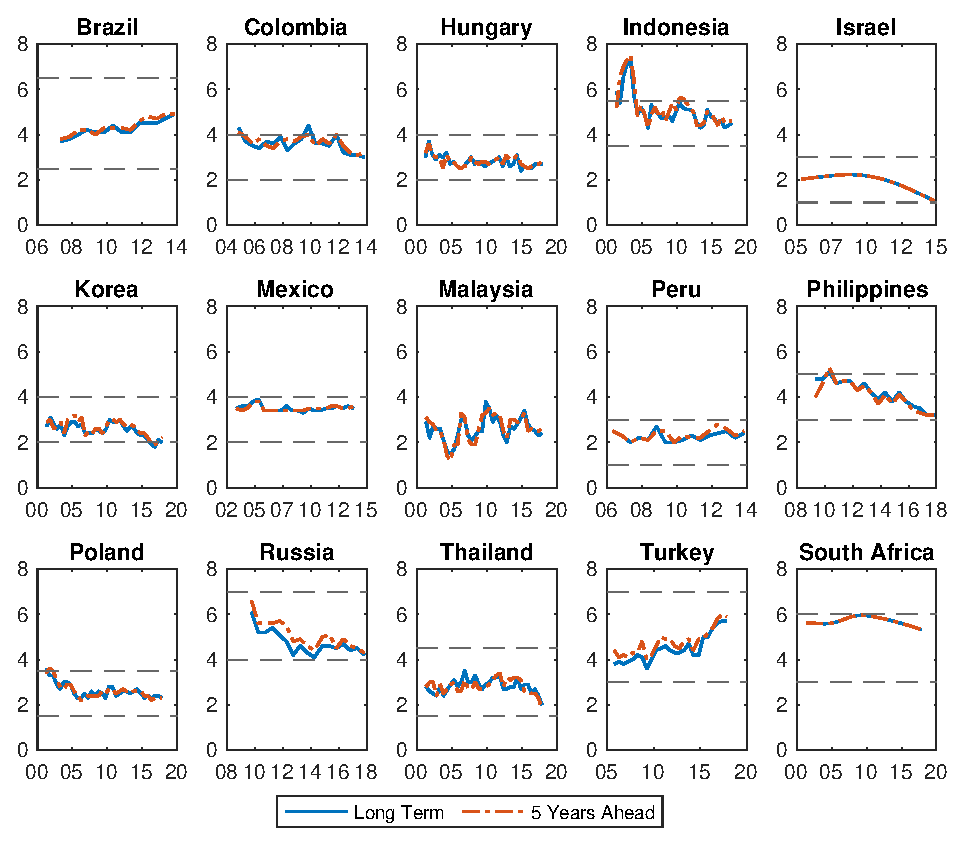
\includegraphics[trim={0cm 0cm 0cm 0cm},clip,height=0.75\textheight,width=\linewidth]{../Figures/Surveys/wnCPI.eps} \\
				\end{center}
				\fignotes{This figure plots the 5-years ahead (dashed line) and the 5- to 10-years ahead or long-term (solid line) average consumer price inflation forecasts against the survey date. For Israel and South Africa, the figure shows the inflation trend, see appendix \ref{sec:trendinf}. The figure also includes the upper and lower bounds for the domestic inflation target, where applicable. The upper and lower bounds are the most recent ones for each country. For Russia, since it has updated its target range almost every year since early 2000s, the plotted band shows the highest and lowest bounds since 2009.}
				\end{minipage}
			\end{center}
		\end{figure}
	\end{landscape}
	}
\end{document}
% trim = {<left> <lower> <right> <upper>}

Although long-term forecasts of future interest rates help to pin down the parameters of the model under the \(\Pmeasure\) measure, \{\(\XmuP, \XPhiP\)\}, there is no source for long-term forecasts for the short rate of emerging markets. 
Nevertheless, they can be inferred from existing data by considering emerging markets as small open economies and using the Fisher equation.  
Specifically, the implied forecast for the nominal short rate (\(\rateSvy\)) equals an expected real interest rate over the same horizon (\(\realrate^{*}\)) plus the expected average inflation reported by Consensus Economics (\(\pi^{CE survey}_{\idxs}\)). 
The first term is in turn equal to the expected global real interest rate in USD plus a real foreign exchange forward premium, akin to equation (\ref{eq:nLCsynt}) but in real terms.
The U.S. real interest rate serves as a proxy for the global real interest rate and is inferred by a combination of survey forecasts of future short-term U.S. Treasury bill yields (\(\srate^{SPF survey}_{\idxs}\)) and future U.S. inflation (\(\pi^{SPF survey}_{\idxs}\)).
Finally, the real forward premium (\(\fwdprm^{\perp}\)) is the residual of regressing the forward premium computed as explained in section \ref{sec:YCsynt} on the expected average inflation from Consensus Economics. 
Thus, the implied forecast for the nominal short rate is obtained as follows
\begin{equation} \label{eq:nRrt}
	\eqrrt 
\end{equation}
The required U.S. data are available quarterly from the Survey of Professional Forecasters.
I use the 5- and 10-year CPI inflation forecasts and, for the T-bill rate, the 10-year forecast and the second longest available one\footnote{ The specific series are CPI5YR, CPI10, BILL10 and TBILLD. The BILL10 series is only released in the first-quarter of a year, so I use linear interpolation for the second to fourth quarters. Consensus Economics forecasts are considered at the end of the month in which they are published; by that time, the most recent value for the U.S. real interest rate forecast is used in equation (\ref{eq:nRrt}).}---since there is no 5-year forecast for the T-bill rate. 
To assess the implied forecasts for the U.S. real rate obtained from surveys, they are compared against the 5- and 10-year zero-coupon real yields constructed by \cite{GSW:2010} who use data from the U.S. TIPS market.
The levels of the two series are comparable. 
TIPS yields are not the benchmark, however, because they are more volatile (their term premium is time varying) and suffer from liquidity problems.
%5Y and 10Y horizon because the plausibility of the SOE assumption is more reasonable in the long term.

Figure \ref{fig:YLD10Y_CBP} shows that the implied long-term forecasts for the short rates are sensible, their level is in line with the synthetic 10-year yield in each country. 
An alternative way to infer the embedded expectations is to use Taylor rule-type regressions for the policy rate.\footnote{For the Taylor rule-type regressions, I regress the policy rate on its lag, the year-on-year consumer price inflation and the year-on-year real GDP growth for all the countries except Israel and South Africa. The coefficient for the lag of the policy rate is a smoothing parameter that improves the fit of the model to the data. I assume that the estimated parameters for inflation and real GDP growth apply at each of the survey maturities. A potential drawback of this approach is precisely that it requires one to know the expectation of the policy rate for the previous forecast horizon. Nevertheless, it is reasonable to assume stationarity for the long-term forecasts (5 and 10 years), in which case only survey data for inflation and GDP growth are needed after dividing their coefficients by 1 minus the coefficient for the lag of the policy rate (due to stationarity). Data for the dependent variable come from the policy rate statistics of the Bank for International Settlements.}
Both approaches yield similar values for the implied forecasts of the short rates. %, the average correlation is 0.75 and 0.83 for the 5- and 10-year tenors, respectively.

\documentclass{article}
\usepackage{graphicx}
\usepackage[margin=1in]{geometry}
\usepackage[outdir=./]{epstopdf}  					% Avoids errors when input figures
\usepackage[labelsep=period,labelfont=bf]{caption}
%\usepackage{subcaption}
\usepackage{afterpage}

\begin{document}
	\afterpage{
	\begin{landscape}
		\begin{figure}[tbph]
			\caption{10-Year Synthetic Yields and Long-Horizon Implied Forecasts of the Short Rate} \label{fig:YLD10Y_CBP}
			\begin{center}								% center the minipage on the line
				\begin{minipage}{0.9\linewidth}
					\begin{center}							% center the figure inside the minipage
						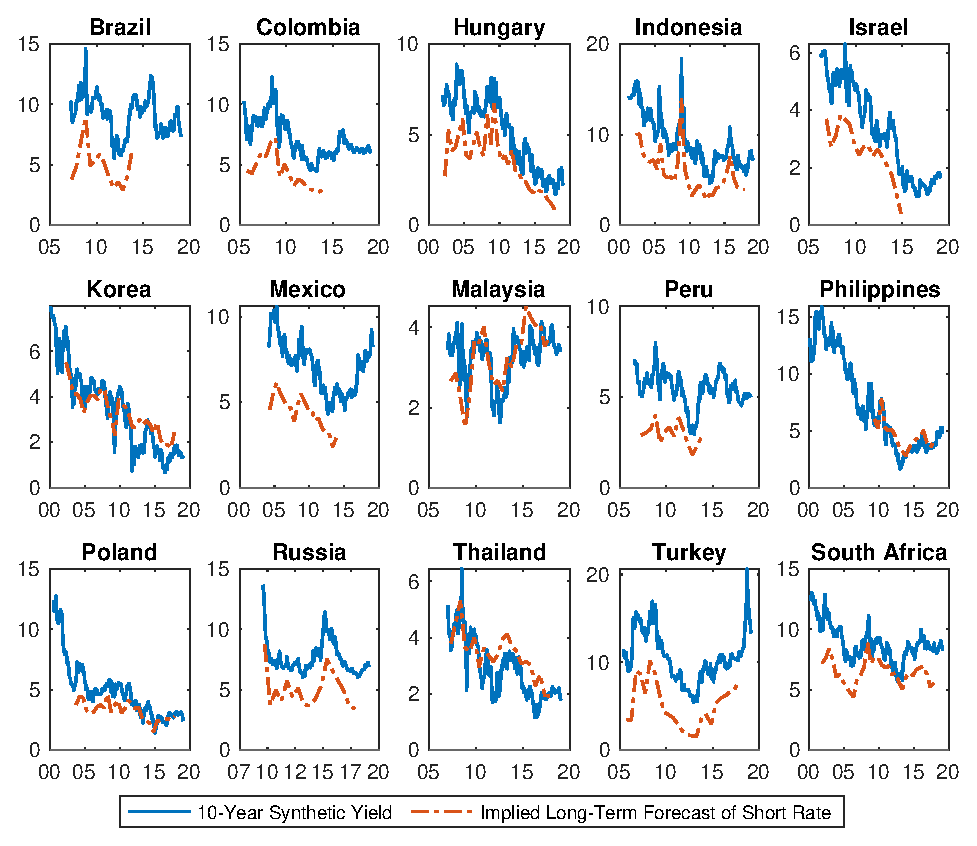
\includegraphics[trim={0cm 0cm 0cm 0cm},clip,height=0.75\textheight,width=\linewidth]{../Figures/Data/YLD10Y_CBP.eps} \\
					\end{center}
					\fignotes{This figure plots the long-horizon implied forecast of the domestic nominal short-term interest rate (dashed line) and the 10-year synthetic yield (solid line). The implied forecast of the short rate is equal to the forecast of the U.S. real short-term interest rate corrected for a real forward premium plus the domestic consumer price inflation forecast, see text for details. The forecast of the U.S. real short-term rate is equal to the difference between the forecast of the three-month U.S. Treasury bill rate and the forecast of the U.S. consumer price inflation.}
				\end{minipage}
			\end{center}
		\end{figure}
	\end{landscape}
	}
\end{document}
% trim = {<left> <lower> <right> <upper>}

To incorporate the information from surveys in the affine model, I assume that the 5-year ahead (inferred) forecast for the short rate of each emerging market guides the expected average short rate under \(\Pmeasure\) given by 
\begin{equation*}
	\yZeroE = \affineAe + \affineBe \Xvars,
\end{equation*}
\noindent in which \(\affineAe = - \frac{1}{\tnr} \affineA\), \(\affineBe = - \frac{1}{\tnr} \affineB\), where in turn \(\affineA = \mathcal{A}(\deltazero, \deltaone, \XmuP, \XPhiP, 0, \tnr)\)\!and \input{../Equations/functionBnE}\!\!; that is, \(\affineAe\) and \(\affineBe\) also satisfy the recursions under the \(\Pmeasure\) measure but with \(\XSigma = 0\) (see appendix C of \cite{Guimaraes:2014}).\footnote{ The difference between \(\yZeroP\) and \(\yZeroE\) is a convexity term due to Jensen's inequality, which increases with maturity. In practice, however, this term usually becomes relevant for maturities beyond ten years. Further, the term is constant across maturities in homoskedastic models like the ones used in this paper.}

Long-term (inferred) forecasts are in turn assumed to be aligned with the 5-year forward rate starting 5 years hence. 
In the model, the forward rate from \(\tnr\) to \(\tnrfwd\) periods hence given by \(\eqyFwd\) becomes 
\begin{equation*}
	\yZeroEfwd = \affineAeFwd + \affineBeFwd \Xvars.
\end{equation*}
\noindent in which \(\eqAeFwd\)  and \(\eqBeFwd\).


\subsection{Estimation} \label{sec:Estimation}
\iftoggle{toclinks}{\gototoc}{} % Turn it on/off in packages.tex, command in macros.tex

The model is estimated using end-of-month data on \textit{risk-free} yield curves; that is, synthetic yields (\(\yLCsynt\)) for emerging markets and nominal yields (\(\yLCnom\)) for advanced economies. 
The estimation for advanced economies is done just for comparison purposes. 

The convergence to the global optimum in affine term structure models estimated by maximum likelihood has been traditionally subject to computational challenges and multiple local optima.
\cite{JSZ:2011} propose a normalization of the affine model that improves the convergence to the global optimum of the likelihood function.

The \cite{JSZ:2011} normalization allows for the near separation of the model's likelihood function into the product of the \(\Pmeasure\) and \(\Qmeasure\) likelihood functions, and reduces the dimension of the parameter space from \((\deltazero, \deltaone, \XmuQ, \XPhiQ, \XSigma)\) to \((\srate^{\Qmeasure}_{\infty}, \lambda^{\Qmeasure},\XSigma)\), where \(\srate^{\Qmeasure}_{\infty}\) is the short rate under \(\Qmeasure\) in the long-run and \(\lambda^{\Qmeasure}\) is a \(\Xdim \times 1\) vector of ordered eigenvalues of \(\XPhiQ\).
It is common to assume that \(\Xdim\) linear combinations of the \(\Ydim\) observed bond yields are measured without error, \(\Xdim < \Ydim\), so that \(\Ydim - \Xdim\) linear combinations of yields are measured with error. 
Following \cite{JSZ:2011}, I consider that the first three principal components---usually referred to as the level, slope and curvature---of the yield curve in each country are the linear combinations of yields measured without error.\footnote{ On average, the first three principal components explain more than 99.5\% of the variation in the synthetic yields of emerging markets and 99.9\% in the nominal yields of advanced economies.} 

The estimation of the affine model follows a two-step procedure. 
The first step uses the \cite{JSZ:2011} normalization. Accordingly, the \(\Pmeasure\) parameters are estimated by OLS of the VAR in equation (\ref{eq:nXvarsP}) using the \(\Xdim\) principal components as pricing factors, which provides initial values for the maximum likelihood estimation of the matrix \(\XSigma\). Then, taking \(\widehat{\Xmu}^{\Pmeasure}\) and \(\widehat{\XPhi}^{\Pmeasure}\) as given, the \(\Qmeasure\) parameters are estimated by maximum likelihood. 
% JSZ needs balanced panels.

In the second step, survey data complement the data on yields. 
This step only applies to emerging markets since the dataset does not include survey data for advanced economies.\footnote{Advanced economies are not the main focus of the paper. In addition, the results reported later for them are more comparable with other studies that do not use survey data. Also, there are less concerns about small sample sizes for advanced economies.} 
The model is augmented with survey data on the last day of the month for which the surveys were published.\footnote{ From 2001 to 2014, data are available in March and September for countries covered in the Eastern European release of Consensus Economics; starting in October 2014, it is released on April and October. For the other emerging markets, forecasts have always been released on April and October.} 
Since survey data from Consensus Economics are available twice a year (whereas yield data for the estimation are monthly), surveys are regarded as missing in non-release dates. 


\subsubsection{Survey-Augmented Model} \label{sec:sATSM}
The Kalman filter is well-suited to handle missing data. 
The transition equation is the law of motion of the pricing factors under the \(\Pmeasure\) measure given in equation (\ref{eq:nXvarsP}). 
The dimension of the observation equation varies depending on the availability of survey data. 

On months in which there is no data on survey expectations, the observation equation adds measurement error to the fitted yields in equation (\ref{eq:nYaffineQ}) for each of the \(\Ydim\) maturities
	\begin{equation} \label{eq:nYaffineY}
	\eqyVecY,
\end{equation}
\noindent in which \(\yVec\) is an \(\Ydim \times 1\) vector of observed bond yields, \(\Avec\) is an \(\Ydim \times 1\) vector with elements \(\affineAQ\), \(\Bvec\) is an \(\Ydim \times \Xdim\) matrix with rows equal to \(\affineBQ\) for \(n = 1, \ldots, \Ydim\), \(\uVec \sim \Normal_\Ydim (0,I) \) and \(\SyVec\) is a lower triangular \(\Ydim \times \Ydim\) matrix with positive elements on the diagonal.

On months when survey data are available, the observation equation increases by the number of survey forecasts \(\Sdim\) as follows 
	\begin{equation} \label{eq:nYaffineYS}
	\begin{bmatrix}
		\yVec \\ 
		\ySVec
	\end{bmatrix} 
	= 
	\begin{bmatrix}
		\Avec \\
		\ASvec
	\end{bmatrix} 
	+
	\begin{bmatrix}
		\Bvec \\
		\BSvec  
	\end{bmatrix} 
	\Xvars
	+
	\begin{bmatrix}
		\SyVec \uVec & \mathbf{0} \\
		\mathbf{0}     & \SsVec \uSVec
	\end{bmatrix} ,
\end{equation}


\noindent in which \(\ySVec\) is an \(\Sdim \times 1\) vector of survey forecasts with elements \(\rateSvy\), \(\ASvec\) is an \(\Sdim \times 1\) vector with elements \(\affineAe\) or \(\affineAeFwd\), \(\BSvec\) is an \(\Sdim \times \Xdim\) matrix with rows equal to \(\affineBe\) or \(\affineBeFwd\) for \(n = 1, \ldots, \Sdim\), \(\uSVec \sim \Normal_\Sdim (0,I) \) and \(\SsVec\) is a lower triangular \(\Sdim \times \Sdim\) matrix with positive elements on the diagonal.

To estimate the survey-augmented model, I follow \cite{Guimaraes:2014} and \cite{Lloyd:2020} in two respects. First, the estimated parameters from the \cite{JSZ:2011} normalization are the initial values for the Kalman filter.
Second, the errors of yields and surveys are assumed to be homoskedastic to reduce the number of parameters to be estimated, so \(\SyVec = \sigma_y I_{\Ydim}\) and \(\SsVec = \sigma_s I_{\Sdim}\), in which \(I_{\Ydim}\) and \(I_{\Sdim}\) are \(\Ydim \times \Ydim\) and \(\Sdim \times \Sdim\) identity matrices. 

It is important to acknowledge that although surveys contain useful information, have good forecasting properties and help anchoring the model to reality, they are not a panacea. 
For instance, surveys might not represent market expectations nor the expectations of the marginal investor,\footnote{Notwithstanding, in the case of the U.S., comparing the 5-year ahead CPI inflation median forecast from the Survey of Professional Forecasters against that from both the Survey of Primary Dealers and the Survey of Market Participants gives, on average, an absolute difference of 5 and 13 basis points, respectively, over the period 2015:I--2020:II.} they might also be subject to measurement error, %\footnote{ In this case, recall that Consensus Economics does not report long-term forecasts for the short rate of emerging markets, so they were inferred from available data.} 
and relying too much on them can be counterproductive as it may lead to overfitting.
Because of this, I consider surveys as imperfect or `noisy' measures of expectations. 
Accordingly, I follow \cite{KimOrphanides:2012} by fixing \(\sigma_s\) at a conservative level of 75 basis points. 


\subsubsection{Estimating Daily Pricing Factors}
\iftoggle{toclinks}{\gototoc}{} % Turn it on/off in packages.tex, command in macros.tex

The analysis of monetary policy spillovers in section \ref{sec:LPs} uses daily changes in nominal and synthetic yields to adequately capture the responses of emerging market yields to surprises in Fed's policy decisions. 
The model, however, is not directly estimated at the daily frequency because there is noise that can undermine the estimation. 

The parameters estimated with monthly data are used to estimate the pricing factors at the daily frequency. 
The Kalman filter maximum likelihood setup explained above gives estimates for both the parameters and the pricing factors. 
I regress the estimated monthly pricing factors on the end-of-month observed yields to obtain the matrix of loadings implied by those pricing factors, and the intercept. 
The matrix of loadings multiplied by the daily yields, plus the intercept, gives an estimate of the daily pricing factors. 
Finally, the estimated parameters (with monthly data) along with the estimated daily pricing factors are used to fit---and decompose---the yields at the daily frequency.

% Theoretically, removing the constant when calculating the log-likelihood is irrelevant. However, it can have an impact in practice because convergence is defined based on the value of the log-likelihood, so the comparison of the convergence against the tolerance criteria can influence whether to stop the loop or continue with more iterations, which will influence the point estimates. Do not need to re-calculate how you report your llk but you may need to adjust your tolerance. Hopefully, if the tolerance is sufficiently small that the difference is not large.

}{}	% Closes \iftoggle{fulldraft}


\section{Decomposing the Yields of Emerging Markets} \label{sec:Decomposition}
\iftoggle{toclinks}{\gototoc}{} % Turn it on/off in packages.tex, command in macros.tex
\iftoggle{cboxes}{	   				  % Turn it on/off in packages.tex
	\begin{boxeditems}
		\item None.
\end{boxeditems}}{}

This section shows that the decompositions of the sovereign yields of emerging markets obtained with the survey-augmented model are sensible. 
It highlights the benefits of using synthetic curves and survey data when analyzing those yields. 
Among the many potential applications of the decompositions, the next section applies them to characterize the transmission channels of U.S. monetary policy to emerging market yields.

\iftoggle{fulldraft}{					% Turn it on/off in packages.tex

\subsection{Model Fit} \label{sec:modelfit}
\iftoggle{toclinks}{\gototoc}{} % Turn it on/off in packages.tex, command in macros.tex

The model fits the data reasonably well.
Figure \ref{fig:s_ylds_bsl_yQ} illustrates the fit of the model for the synthetic yields. 
The focus is on the 10-year maturity for the sake of brevity. 
The squared root of the average (across months and maturities) squared difference between the actual and the fitted yields is commonly used to summarize the fitting errors. 
The average fitting error for the synthetic yields of emerging markets is 17 basis points, a reasonable fit. For reference, the average fitting error for the nominal yields of the advanced economies in the sample is 5 basis points, in line with previous studies \citep{Wright:2011}. 
The dynamics of emerging market yields are thus relatively harder to capture.\footnote{ Notwithstanding, it is important to keep in mind that for some countries, large fitting errors might be an indication of less liquid and deep markets.} 
%\cite{HuPanWang:2013} propose to use cross-sectional pricing errors in U.S. Treasuries as a measure of market illiquidity.
%it simply means the model is not as good a cross-sectional fit for some emerging markets. Maybe there is a missing factor that picks up shallow markets, but perhaps inflation dynamics in those countries are not captured by VAR(1) dynamics. 

\documentclass{article}
\usepackage{graphicx}
\usepackage[margin=1in]{geometry}
\usepackage[outdir=./]{epstopdf}  					% Avoids errors when input figures
\usepackage[labelsep=period,labelfont=bf]{caption}
%\usepackage{subcaption}

\begin{document}
	\begin{figure}[tbph]
		\caption{Model Fit for Emerging Markets: 10-Year Synthetic Yields} \label{fig:s_ylds_bsl_yQ}
		\begin{center}								% center the minipage on the line
			\begin{minipage}{0.9\linewidth}
				\begin{center}							% center the figure inside the minipage
					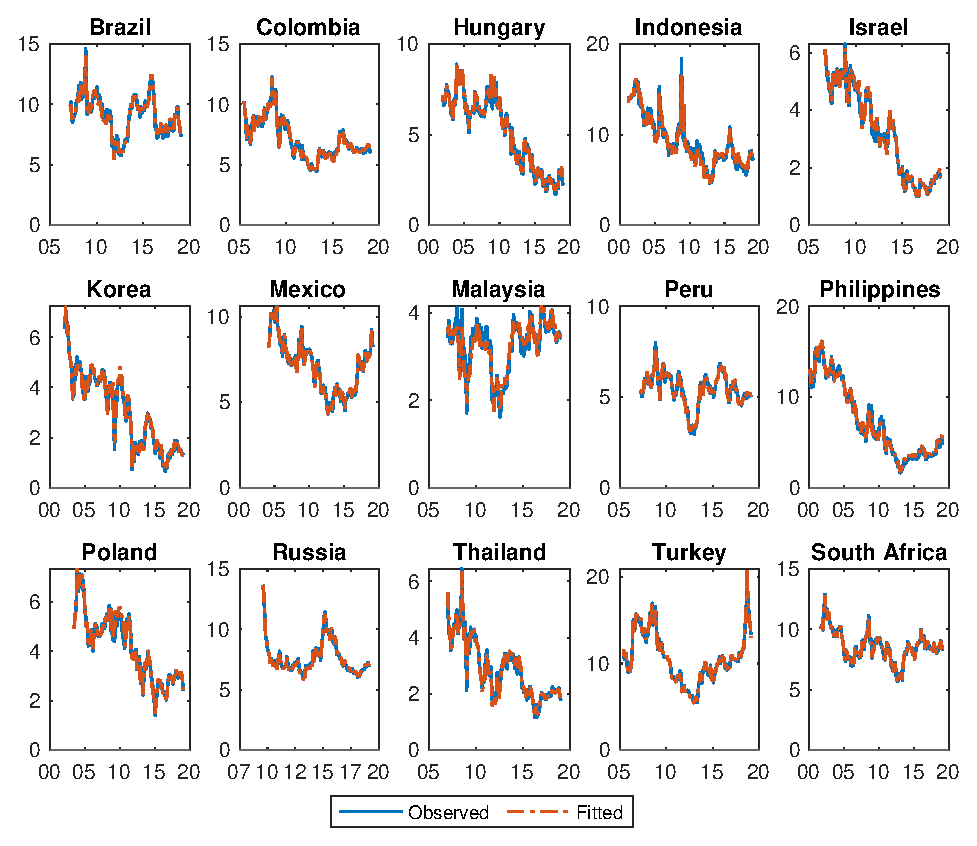
\includegraphics[trim={0cm 0cm 0cm 0cm},clip,height=0.86\textheight,width=\linewidth]{../Figures/Estimation/s_ylds_bsl_yQ.eps} \\
				\end{center}
				\fignotes{This figure plots the fitted (dashed line) and the actual (solid line) 10-year synthetic yields. The fitted yield is obtained after estimating the survey-augmented affine term structure model.}
			\end{minipage}
		\end{center}
	\end{figure}
\end{document}
% trim = {<left> <lower> <right> <upper>}


\subsection{Decomposition Assessment}
\iftoggle{toclinks}{\gototoc}{} % Turn it on/off in packages.tex, command in macros.tex

The estimation of the model allows to decompose the yields of emerging markets into three parts, as explained in section \ref{sec:ATSM}. 
Broad patterns are discussed before assessing each component individually. 

Table \ref{tab:dcmpstats} summarizes the decomposition of the nominal yields of emerging markets.\footnote{ The decompositions for advanced economies are not displayed for two reasons. First, they have already been studied before, see for instance \cite{Wright:2011} and \cite{ACDM:2019}. Second, the dataset does not include survey data for advanced economies and so their decompositions may not be robust. They are nonetheless a useful benchmark to assess some results (e.g., average fitting errors above).} 
Average expected short rates are the main component of nominal yields. 
Meanwhile, the relevance of the term premium increases with maturity, whereas the credit risk compensation is broadly stable. 
On average, the three parts respectively represent around 56, 31 and 13\% of the 10-year nominal yields of emerging markets, which indicates that the term premium plays a relatively bigger role than the credit risk compensation.

\documentclass[a4paper,12pt]{article}
\usepackage[labelsep=period,labelfont=bf]{caption}
\usepackage{multirow}
\usepackage{booktabs}
\usepackage{threeparttable}
\usepackage{pdflscape}
\usepackage{tabularx}
%\usepackage[margin=1in]{geometry}
%%% Personalized Macros
% Definitions, Equations, Table of Contents, Tables, Subcaptions, Paths, Text Fomats

%-------------------------------------------------------------------
% Variable Definitions
%-------------------------------------------------------------------
\providecommand{\tnr}{n}
\providecommand{\tnrfwd}{m}
\providecommand{\idxt}{t}
\providecommand{\idxi}{i}
\providecommand{\idxh}{h}
\providecommand{\idxs}{\idxt,\tnr}
\providecommand{\idxsfwd}{\tnr | \tnrfwd}
\providecommand{\idxsfwdt}{\idxt,\idxsfwd}
\providecommand{\idxspnl}{\idxi,\idxt}
\providecommand{\idxspnlfwd}{\idxi,{\idxt+\idxh}}
\providecommand{\idxspnllag}{\idxi,{\idxt-1}}
\providecommand{\idxspnllaglag}{\idxi,{\idxt-j}}
\providecommand{\fInst}{f_{\idxs}}
\providecommand{\yld}{y}
\providecommand{\xpc}{e}
\providecommand{\yZero}{\yld_{\idxs}}
\providecommand{\yZeroQ}{\yZero^{\Qmeasure}}
\providecommand{\yZeroP}{\yZero^{\Pmeasure}}
\providecommand{\yZeroE}{\yZero^{\xpc}}
\providecommand{\yZeroFwd}{\frate_{\idxsfwdt}}
\providecommand{\yZeroEfwd}{\yZeroFwd^{\xpc}}
\providecommand{\Pzero}{P_{\idxs}}
\providecommand{\Pzerolag}{P_{\idxt+1,\tnr-1}}
\providecommand{\srate}{i}
\providecommand{\shortrate}{\srate_{\idxt}}
\providecommand{\shortratelag}{\srate_{\idxt-1}}
\providecommand{\frate}{f}
\providecommand{\realrate}{r_{\idxs}}
\providecommand{\rateSvy}{\srate_{\idxs}^{survey}}
\providecommand{\SDF}{M_{\idxt+1}}
\providecommand{\SDFprod}{\ExpP \left[\Pi_{j=1} ^\tnr M_{\idxt+j}\right]}
\providecommand{\SDFsum}{\ExpQ \left[\exp \left(- \Sigma_{j=0} ^{\tnr-1} \srate_{\idxt+j} \right) \right]}
\providecommand{\Xvars}{X_{\idxt}}
\providecommand{\XvarsFwd}{X_{\idxt+1}}
\providecommand{\affineA}{A_{\tnr}}
\providecommand{\affineB}{B_{\tnr}}
\providecommand{\affineAfwd}{A_{\tnr + 1}}
\providecommand{\affineBfwd}{B_{\tnr + 1}}
\providecommand{\affineAQ}{\affineA^{\Qmeasure}}
\providecommand{\affineBQ}{\affineB^{\Qmeasure}}
\providecommand{\affineAP}{\affineA^{\Pmeasure}}
\providecommand{\affineBP}{\affineB^{\Pmeasure}}
\providecommand{\affineAe}{\affineA^{\xpc}}
\providecommand{\affineBe}{\affineB^{\xpc}}
\providecommand{\affineAeFwd}{A_{\idxsfwd}^{\xpc}}
\providecommand{\affineBeFwd}{B_{\idxsfwd}^{\xpc}}
\providecommand{\yLCnom}{\yld_{\idxs} ^{LC}}
\providecommand{\yLCsynt}{\widetilde{\yld}_{\idxs} ^{LC}}
\providecommand{\yUS}{y_{\idxs} ^{US}}
\providecommand{\yUSsynt}{\widetilde{\yld}_{\idxs} ^{US}}
\providecommand{\fx}{\mathit{s}}

% Math fonts
\providecommand{\Xdim}{\mathrm{K}}
\providecommand{\Ydim}{\mathrm{N}}
\providecommand{\Sdim}{\mathrm{S}}
\providecommand{\Normal}{\mathcal{N}}
\providecommand{\Pmeasure}{\mathbb{P}}
\providecommand{\Qmeasure}{\mathbb{Q}}
\providecommand{\Expec}{\mathrm{E}_{t}}
\providecommand{\ExpP}{\mathrm{E}^{\Pmeasure}_{t}}
\providecommand{\ExpQ}{\mathrm{E}^{\Qmeasure}_{t}}
\providecommand{\Svy}{S}
\providecommand{\yVec}{\mathbf{\yld}_{t}}
\providecommand{\ySVec}{\yVec^{\Svy}}
\providecommand{\Avec}{\mathbf{A}}
\providecommand{\Bvec}{\mathbf{B}}
\providecommand{\ASvec}{\mathbf{A}^{\Svy}}
\providecommand{\BSvec}{\mathbf{B}^{\Svy}}
\providecommand{\uVec}{\mathbf{u}_{t}}
\providecommand{\uSVec}{\mathbf{u}_{t}^{\Svy}}
\providecommand{\Svec}{\mathbf{\Sigma}}
\providecommand{\SyVec}{\mathbf{\Svec}_{Y}}
\providecommand{\SsVec}{\mathbf{\Svec}_{\Svy}}

% Greeks
\providecommand{\termprm}{\tau_{\idxs}}
\providecommand{\riskprice}{\lambda_{t}}
\providecommand{\lambdazero}{\lambda_{0}}
\providecommand{\lambdaone}{\lambda_{1}}
\providecommand{\fwdprm}{\rho_{\idxs}}
\providecommand{\CIPdev}{\phi_{\idxs}}
\providecommand{\deltazero}{\delta_{0}}
\providecommand{\deltaone}{\delta_{1}}
\providecommand{\error}{\nu_{t+1}}
\providecommand{\errorQ}{\error^{\Qmeasure}}
\providecommand{\errorP}{\error^{\Pmeasure}}
\providecommand{\XmuP}{\mu^{\Pmeasure}}
\providecommand{\XmuQ}{\mu^{\Qmeasure}}
\providecommand{\XSigma}{\Sigma}
\providecommand{\XPhiP}{\Phi^{\Pmeasure}}
\providecommand{\XPhiQ}{\Phi^{\Qmeasure}}
\providecommand{\betaLT}{\beta_{0}}
\providecommand{\betaST}{\beta_{1}}
\providecommand{\betaMTns}{\beta_{2}}
\providecommand{\betaMTnss}{\beta_{3}}
\providecommand{\tauNS}{\tau_{1}}
\providecommand{\tauNSS}{\tau_{2}}
\providecommand{\tnrTauNS}{\tnr/\tauNS}
\providecommand{\tnrTauNSS}{\tnr/\tauNSS}
\providecommand{\params}{\theta}
\providecommand{\Vasy}{\Omega}
\providecommand{\cmpnt}{\Psi}
\providecommand{\Jacobian}{\Gamma}
\providecommand{\Hessian}{\mathcal{H}_\params}
\providecommand{\asydstr}{\sqrt{\Ydim} \left( \widehat{\cmpnt} - \cmpnt \right) \xrightarrow[]{d} \Normal \left(0,\, \Jacobian \, \Vasy \, \Jacobian' \right)}
\providecommand{\sampleHjoint}{\frac{1}{\Ydim} \frac{\partial^{2} \ell_{\Ydim} (\widehat{\params})}{\partial \params \partial \params'}}
\providecommand{\sampleHindiv}{\frac{1}{\Ydim} \sum_{i = 1}^{\Ydim} \frac{\partial^{2} \log \mathit{f} (X_{i} | \widehat{\params})}{\partial \params \partial \params'}}

% Nelson-Siegel_Svensson
\providecommand{\loadSTnsFwd}{\exp\left(-\tnrTauNS \right)}
\providecommand{\loadSTnssFwd}{\exp\left(-\tnrTauNSS \right)}
\providecommand{\loadMTnsFwd}{\left(\tnrTauNS\right) \loadSTnsFwd}
\providecommand{\loadMTnssFwd}{\left(\tnrTauNSS\right) \loadSTnssFwd}
\providecommand{\loadSTnsZero}{\frac{1-\loadSTnsFwd}{\tnrTauNS}}
\providecommand{\loadSTnssZero}{\frac{1-\loadSTnssFwd}{\tnrTauNSS}}
\providecommand{\loadMTnsZero}{\left(\loadSTnsZero - \loadSTnsFwd \right)}
\providecommand{\loadMTnssZero}{\left( \loadSTnssZero - \loadSTnssFwd \right)}

%\providecommand{\}{}
% DELETE in a later revision
\providecommand{\Xmu}{\mu}
\providecommand{\XPhi}{\Phi}
\providecommand{\XmuStar}{\mu^{*}}
\providecommand{\XPhiStar}{\Phi^{*}}
\providecommand{\STrate}{r}
\providecommand{\rShort}{\STrate_{t}}
\providecommand{\rShortlag}{\STrate_{t-1}}
\providecommand{\ySvy}{\STrate_{\idxs}^{survey}}
\providecommand{\TPatsm}{tp_{\idxs}}

%-------------------------------------------------------------------
% Equations
%-------------------------------------------------------------------
\newcommand{\eqyLCsynt}{\yLCsynt = \yUS + \fwdprm}
\newcommand{\eqCIPdevDS}{\CIPdev = \yLCnom - \yLCsynt}
\newcommand{\eqCIPdevQ}{\CIPdev = \yLCnom - \yZeroQ}

\newcommand{\PzeroP}{\Pzero = \ExpP \left[ \SDF \Pzerolag \right]}
\newcommand{\PzeroQ}{\Pzero = \ExpQ \left[ \exp\left(- \shortrate\right) \Pzerolag \right]}

\newcommand{\eqXvarsFwdQ}{\XvarsFwd = \XmuQ + \XPhiQ \Xvars  + \XSigma \errorQ}
\newcommand{\eqshortrate}{\shortrate = \deltazero + \deltaone' \Xvars}
\newcommand{\eqyZeroP}{\yZeroP = \affineAP + \affineBP \Xvars}
\newcommand{\eqyZeroQ}{\yZeroQ = \affineAQ + \affineBQ \Xvars}
\newcommand{\eqTP}{\termprm = \yZeroQ - \yZeroP}
\newcommand{\eqXvarsFwdP}{\XvarsFwd = \XmuP + \XPhiP \Xvars  + \XSigma \errorP}
\newcommand{\eqriskprice}{\riskprice = \lambdazero + \lambdaone \Xvars}
\newcommand{\eqSDF}{\SDF = \exp\left( -\shortrate -\frac{1}{2} \riskprice' \riskprice - \riskprice' \errorP \right)}
%\newcommand{}{}

\newcommand{\eqpanelUCSV}{\tau_{\idxspnl} = \alpha_{\idxi} + \beta_{1} \sigma^{\pi}_{\idxspnl} + \beta_{2} GDP_{\idxspnl} + u_{\idxspnl}}
\newcommand{\eqpanelTPreg}{\yld_{\idxspnl} = \alpha_{\idxi} + \gamma_{1}' z^{1}_{\idxspnl} + \gamma_{2}' z^{2}_{\idxspnl} + u_{\idxspnl}}
\newcommand{\eqySvy}{\rateSvy = \frac{\widehat{\beta}_{0}}{1-\widehat{\beta}_{\srate}} + \frac{\widehat{\beta}_{{\pi}}}{1-\widehat{\beta}_{\srate}} \pi_{\idxs}^{survey} + \frac{\widehat{\beta}_{{g}}}{1-\widehat{\beta}_{\srate}} g_{\idxs}^{survey} }

\newcommand{\eqyFwd}{\yZeroFwd = \left( \tnrfwd \yld_{\idxt,\tnrfwd} - \tnr \yZero \right)/ \left( \tnrfwd - \tnr \right) }
\newcommand{\eqAeFwd}{\affineAeFwd = \left( \tnrfwd A_{\tnrfwd}^{\xpc}  - \tnr \affineAe \right)/ \left( \tnrfwd - \tnr \right) }
\newcommand{\eqBeFwd}{\affineAeFwd = \left( \tnrfwd B_{\tnrfwd}^{\xpc}  - \tnr \affineBe \right)/ \left( \tnrfwd - \tnr \right) }
\newcommand{\eqrrt}{\rateSvy = \realrate^{*} + \pi^{e}_{\idxs} = \left( \srate^{SPF survey}_{\idxs} - \pi^{SPF survey}_{\idxs} \right) + \fwdprm^{\perp} + \pi^{CE survey}_{\idxs} }


\newcommand{\eqyVecY}{\yVec = \Avec + \Bvec \Xvars + \SyVec \uVec}
\newcommand{\eqyVecS}{\ySVec = \ASvec + \BSvec \Xvars + \SsVec \uSVec}

% One shock at a time
%\newcommand{\eqpanelLP}{\yld_{\idxspnlfwd} - \yld_{\idxspnllag} = \alpha_{\idxh,\idxi} + \beta_{\idxh} \epsilon_{\idxt} + \gamma_{\idxh} \Delta \yld_{\idxspnllag} + \phi_{\idxh} \fx_{\idxspnllag}  + u_{\idxspnlfwd}}

% All shocks at once
\newcommand{\eqpanelLP}{\yld_{\idxspnlfwd} - \yld_{\idxspnllag} = \alpha_{\idxh,\idxi} + \sum^{3}_{j = 1} \beta^{j}_{\idxh} \epsilon^{j}_{\idxt} + \gamma_{\idxh} \Delta \yld_{\idxspnllag} + \eta_{\idxh} \fx_{\idxspnllag}  + u_{\idxspnlfwd}} 

\newcommand{\eqpanelLPlevels}{\yld_{\idxspnlfwd} = \alpha_{\idxh,\idxi} + \sum^{3}_{j = 1} \beta^{j}_{\idxh} \epsilon^{j}_{\idxt} + \sum^{2}_{j = 1} \gamma^{j}_{\idxh} \yld_{\idxspnllaglag} + \eta_{\idxh} \fx_{\idxspnllag}  + u_{\idxspnlfwd}} 
% \beta^{target}_{\idxh} \epsilon^{target}_{\idxt} + \beta^{path}_{\idxh} \epsilon^{path}_{\idxt} + \beta^{lsap}_{\idxh} \epsilon^{lsap}_{\idxt} 

%---------------------------------------------------------------
% Table of Contents
%---------------------------------------------------------------
% Link to ToC from section
\newcommand{\gototoc}{\vspace{-2cm} \null\hfill [\hyperlink{toc}{Go2ToC}] \newline}

% Link back to section from ToC
\newcommand{\maketoc}{
	\hypertarget{toc}{}
	\newpage
	\tableofcontents
	\vspace{2.5\bigskipamount} }

% Box with bullets for tasks to do in a section
\newenvironment{boxeditems}
	{\begin{tabular}{|p{\linewidth}|}
	\hline
	\begin{itemize}
	}
	{
	\end{itemize}
	\\ \hline
	\end{tabular} \\
	}

%---------------------------------------------------------------
% Tables: Estout Commands following Jörg Weber
%---------------------------------------------------------------
\newcommand{\sym}[1]{\rlap{#1}}

\let\estinput=\input	% define new input command to flatten the document

\newcommand{\estauto}[2]{
	\newcolumntype{C}{>{\centering\arraybackslash}X}
	\vspace{.75ex}{
%		\begin{tabularx}{1.4\textwidth}{l*{#2}C}
		\begin{tabularx}{0.95\linewidth}{l*{#2}C}
			\toprule
			\estinput{#1}
			\\ \bottomrule
			\addlinespace[.75ex]
		\end{tabularx}
	}
}

% Allow line breaks with \\ in specialcells
\newcommand{\specialcell}[2][c]{\begin{tabular}[#1]{@{}c@{}}#2\end{tabular}}

%---------------------------------------------------------------
% Subcaptions
%---------------------------------------------------------------
% Notes after figures following Jörg Weber
\newcommand{\figtext}[1]{
	\vspace{-1ex}
	\captionsetup{justification=justified,font=footnotesize}
	\caption*{#1}
%	\captionsetup{justification=raggedright,singlelinecheck=false,font=footnotesize}
%	\caption*{\hspace{6pt}\hangindent=1.5em #1}
}

\newcommand{\fignote}[1]{\figtext{\emph{Note:~}~#1}}
\newcommand{\fignotes}[1]{\figtext{\emph{Notes:~}~#1}}

% Notes after tables
\newcommand{\tabnote}[1]{
	\begin{tablenotes}[para,flushleft]
		\footnotesize \emph{Notes:~}~#1
	\end{tablenotes}
}

%---------------------------------------------------------------
% Paths
%---------------------------------------------------------------
%\newcommand*{\pathFigs}{../Figures}
%\input{pathFigs/fig1.tex}

%---------------------------------------------------------------
% Text Fomats
%---------------------------------------------------------------
%\newcommand{\txtbi}[1]{\textbf{\textit{#1}}}

%---------------------------------------------------------------
% Other
%---------------------------------------------------------------
%\newcommand\LL[1]{\multicolumn{2}{|l}{#1}}
%\newcommand\RR[1]{\multicolumn{2}{c|}{#1}}
%\newcommand\LR[1]{\multicolumn{2}{|c|}{#1}}
%\newcommand\LL[1]{\multicolumn{1}{|c}{#1}}
%\newcommand\RR[1]{\multicolumn{1}{c|}{#1}}
%\newcommand\LR[1]{\multicolumn{1}{|c|}{#1}}

\begin{document}
	\begin{normalsize}
%		\begin{landscape}
			\begin{table}
				\begin{center}
					\caption{Descriptive Statistics for the Decomposition of Yields of Emerging Markets} \label{tab:dcmpstats}
					\begin{threeparttable}
						\estauto{../Tables/f_dcmpstats.tex}{6}
						\tabnote{This table reports the average, the standard deviation, the minimum and the maximum values using end-of-month data for different tenors of the components of the emerging market nominal yields. All figures are expressed in annualized percentage points.}
					\end{threeparttable}
				\end{center}
			\end{table}
%		\end{landscape}
	\end{normalsize}
\end{document}

Figure \ref{fig:ny_dcmp} shows the decomposition of the \(10\)-year yield for each country. Two patterns emerge from the figure. 
First, the term premium and the credit risk compensation are time-varying and both play an important role in the dynamics of the yields. 
Although their relative importance varies by country, the term premium indeed plays a relatively bigger role, in general. 
Second, there is a downward trend in the expected future short rate and the term premium of several countries, consistent with the evidence for advanced economies \citep{Wright:2011,ACDM:2019}.

\documentclass{article}
\usepackage{graphicx}
\usepackage[margin=1in]{geometry}
\usepackage[outdir=./]{epstopdf}  					% Avoids errors when input figures
\usepackage[labelsep=period,labelfont=bf]{caption}
%\usepackage{subcaption}

\begin{document}
	\afterpage{
	\begin{landscape}
		\begin{figure}[tbph]
			\caption{Decomposition of the 10-Year Nominal Yields of Emerging Markets} \label{fig:ny_dcmp}
			\begin{center}								% center the minipage on the line
				\begin{minipage}{0.9\linewidth}
					\begin{center}							% center the figure inside the minipage
						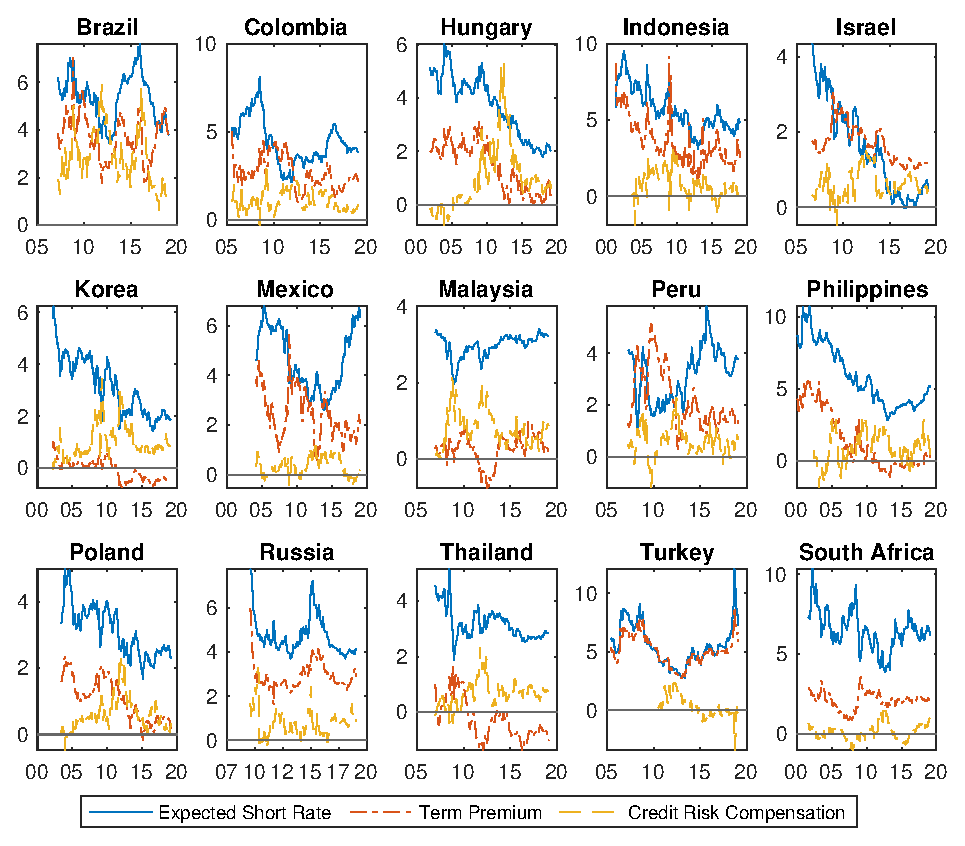
\includegraphics[trim={0cm 0cm 0cm 0cm},clip,height=0.8\textheight,width=\linewidth]{../Figures/Estimation/ny_dcmp.eps} \\
					\end{center}
					\fignotes{This figure plots the components of the 10-year nominal yields of emerging markets. The yields are decomposed into an average expected future short-term interest rate (solid line), a term premium (dash-dotted line) and a credit risk compensation (dashed line).}
				\end{minipage}
			\end{center}
		\end{figure}
	\end{landscape}
	}
\end{document}
% trim = {<left> <lower> <right> <upper>}

In addition, the results for individual countries are consistent with their particular circumstances.
For instance, the expected short rate in Mexico increased during the tightening cycle that started following the 2016 U.S. presidential election, after which market participants expected a deterioration in the bilateral relation.
The credit risk compensation for Hungary increased after 2010, when the current populist government came into power, and around the European sovereign debt crisis. 
In Poland, the term premium declined after the global financial crisis as in other European countries in response to the unconventional monetary policies of the European Central Bank. 


\subsubsection{Average Expected Future Short Rate}
\iftoggle{toclinks}{\gototoc}{} % Turn it on/off in packages.tex, command in macros.tex

Figure \ref{fig:bsl_yP_scbp} shows that the model-implied 10-year average expected future short rate aligns reasonably well with the (inferred) long-term forecast for the short rate, even though the model does not rely too much on surveys given the conservative value for \(\sigma_s\) of 75 basis points. 
All the results later on are based on this conservative value but, as a reference, when \(\sigma_s\) is estimated, its average value across all emerging markets is 31 basis points.
%When no survey data is used in the estimation, the model-implied expectations are weakly connected to the forecasts.

\documentclass{article}
\usepackage{graphicx}
\usepackage[margin=1in]{geometry}
\usepackage[outdir=./]{epstopdf}  					% Avoids errors when input figures
\usepackage[labelsep=period,labelfont=bf]{caption}
%\usepackage{subcaption}

\begin{document}

\begin{figure}[tbph]
	\begin{center}
		\caption{Interest Rate Forecasts vs Model-Implied Expectation: 10-Year Yields}
		\label{fig:bsl_yP_scbp}
		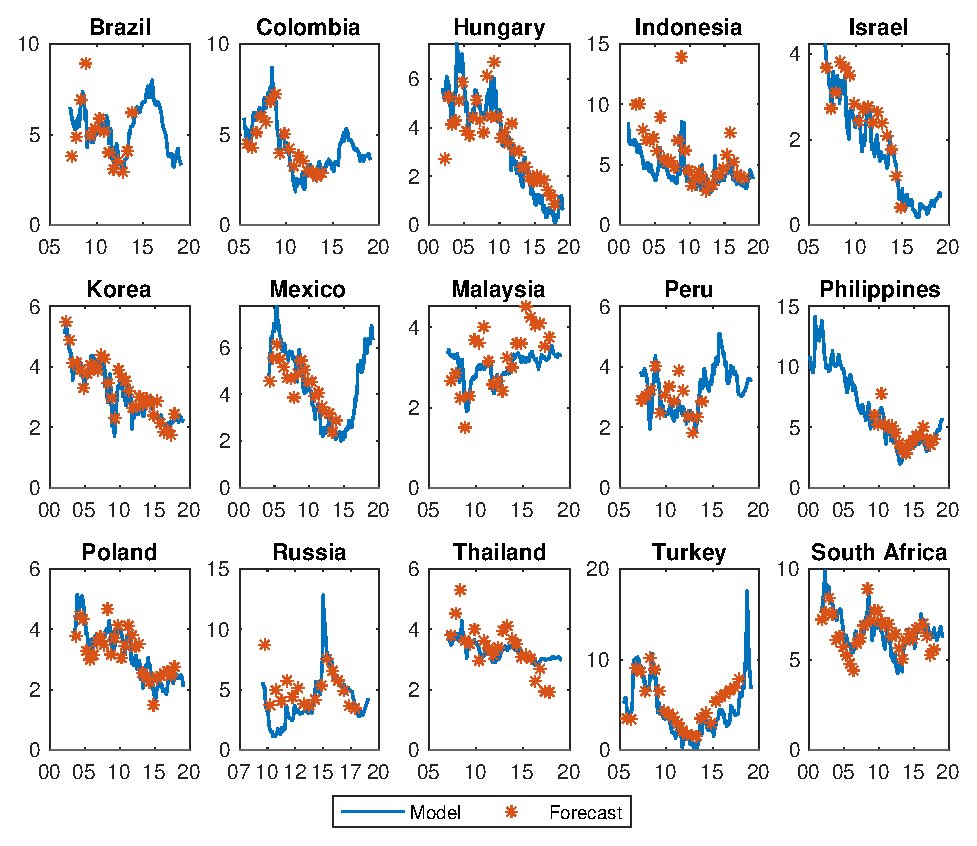
\includegraphics[trim={0cm 0cm 0cm 0cm},clip,height=1\textheight,width=1.4\textwidth]{../Figures/Estimation/bsl_yP_scbp.eps} \\
	\end{center}
	% trim = {<left> <lower> <right> <upper>}
%	\vspace{-0.4cm} \caption*{\footnotesize{\textit{Notes}: Notes.}}
\end{figure}

\end{document}


\subsubsection{Term Premium} \label{sec:TP}
\iftoggle{toclinks}{\gototoc}{} % Turn it on/off in packages.tex, command in macros.tex

While the (bond) risk premium is sometimes associated with the term premium in advanced economies, the two concepts are different in emerging markets. 
The purpose of leveraging on synthetic yields (and surveys) is to estimate a genuine term premium, clean of credit risk. 
This subsection assesses the sensibility of this `clean' term premium.

A simple robustness check for the model-implied term premium is to compare it against an alternative measure. 
The survey-based term premium is a model-free measure equal to the difference between the \textit{synthetic} yield and the short rate forecast over the same horizon. 
Since the model-implied expectations track the short rate forecasts closely (see figure \ref{fig:bsl_yP_scbp}), the two measures of term premia comove positively, with an average correlation of 0.52 across countries for the 10-year maturity. 
%corr dtp120m scbp120m if em
%(obs=346)
%				|  dtp120m scbp120m
%-------------+------------------
%dtp120m |   1.0000
%scbp120m |   0.5219   1.0000

Another test is to see whether the term premium is related to inflation uncertainty.
\cite{Wright:2011} documents a downward trend in the term premia of advanced economies and argues that it owes in part to a reduction in inflation uncertainty. 
%The term premia in EMs is generally higher than the term premia in AEs.
Since inflation in emerging markets tends to be higher and more volatile than in advanced economies \citep{HaKoseOhnsorge:2019}, it is reasonable to assume that the relationship between term premia and inflation uncertainty is particularly relevant in emerging markets. 
To test this hypothesis, I run the following panel regressions %for different maturities 
\begin{equation} \label{eq:nPanelUCSV}
	\eqpanelUCSV ,
\end{equation}
\noindent in which \(\alpha_{\idxi}\) are country fixed effects, \(\sigma^{\pi}_{\idxspnl}\) is a measure of inflation uncertainty, \(GDP_{\idxspnl}\) is the domestic real GDP growth to control for the business cycle, 
and \(u_{\idxspnl}\) is the error term. 
The dependent variable \(\tau_{\idxspnl}\) is the model-implied term premium at different maturities.
Following \cite{Wright:2011}, the measure of inflation uncertainty is the standard deviation of the permanent component of inflation in the Stock--Watson unobserved components stochastic volatility (UCSV) model, estimated using quarterly data for each country.\footnote{ The UCSV model assumes that inflation has permanent and transitory components subject to uncorrelated shocks that vary over time.} 
%monthly data shows that inflation is negatively autocorrelated which messes the results
To test for significance, I use the Driscoll--Kraay estimator that allows the errors to be correlated across countries and over time.\footnote{ The Pesaran test of cross-sectional independence is rejected in all cases at the 1\% significance level.} 
% Lag selection based on Newey \& West(1994) “plug-in” estimator
%Automatic lag selection in covariance matrix estimation. Review of Economic Studies 61: 631–653.

Table \ref{tab:tpucsv} shows that the term premium and the standard deviation of the permanent component are positively associated. The relationship is significant for medium- and long-term maturities, 
and the relevance increases with maturity.
The results become stronger after controlling for the business cycle. 
Although this specification might be subject to econometric problems, since it involves persistent variables and ignores measurement error, the results are aligned with the view that the term premium compensates investors for bearing inflation uncertainty in emerging markets too.

\documentclass[a4paper,12pt]{article}
\usepackage[labelsep=period,labelfont=bf]{caption}
\usepackage{multirow}
\usepackage{booktabs}
\usepackage{threeparttable}
\usepackage{pdflscape}
\usepackage{tabularx}
%\usepackage[margin=1in]{geometry}
%%% Personalized Macros
% Definitions, Equations, Table of Contents, Tables, Subcaptions, Paths, Text Fomats

%-------------------------------------------------------------------
% Variable Definitions
%-------------------------------------------------------------------
\providecommand{\tnr}{n}
\providecommand{\tnrfwd}{m}
\providecommand{\idxt}{t}
\providecommand{\idxi}{i}
\providecommand{\idxh}{h}
\providecommand{\idxs}{\idxt,\tnr}
\providecommand{\idxsfwd}{\tnr | \tnrfwd}
\providecommand{\idxsfwdt}{\idxt,\idxsfwd}
\providecommand{\idxspnl}{\idxi,\idxt}
\providecommand{\idxspnlfwd}{\idxi,{\idxt+\idxh}}
\providecommand{\idxspnllag}{\idxi,{\idxt-1}}
\providecommand{\idxspnllaglag}{\idxi,{\idxt-j}}
\providecommand{\fInst}{f_{\idxs}}
\providecommand{\yld}{y}
\providecommand{\xpc}{e}
\providecommand{\yZero}{\yld_{\idxs}}
\providecommand{\yZeroQ}{\yZero^{\Qmeasure}}
\providecommand{\yZeroP}{\yZero^{\Pmeasure}}
\providecommand{\yZeroE}{\yZero^{\xpc}}
\providecommand{\yZeroFwd}{\frate_{\idxsfwdt}}
\providecommand{\yZeroEfwd}{\yZeroFwd^{\xpc}}
\providecommand{\Pzero}{P_{\idxs}}
\providecommand{\Pzerolag}{P_{\idxt+1,\tnr-1}}
\providecommand{\srate}{i}
\providecommand{\shortrate}{\srate_{\idxt}}
\providecommand{\shortratelag}{\srate_{\idxt-1}}
\providecommand{\frate}{f}
\providecommand{\realrate}{r_{\idxs}}
\providecommand{\rateSvy}{\srate_{\idxs}^{survey}}
\providecommand{\SDF}{M_{\idxt+1}}
\providecommand{\SDFprod}{\ExpP \left[\Pi_{j=1} ^\tnr M_{\idxt+j}\right]}
\providecommand{\SDFsum}{\ExpQ \left[\exp \left(- \Sigma_{j=0} ^{\tnr-1} \srate_{\idxt+j} \right) \right]}
\providecommand{\Xvars}{X_{\idxt}}
\providecommand{\XvarsFwd}{X_{\idxt+1}}
\providecommand{\affineA}{A_{\tnr}}
\providecommand{\affineB}{B_{\tnr}}
\providecommand{\affineAfwd}{A_{\tnr + 1}}
\providecommand{\affineBfwd}{B_{\tnr + 1}}
\providecommand{\affineAQ}{\affineA^{\Qmeasure}}
\providecommand{\affineBQ}{\affineB^{\Qmeasure}}
\providecommand{\affineAP}{\affineA^{\Pmeasure}}
\providecommand{\affineBP}{\affineB^{\Pmeasure}}
\providecommand{\affineAe}{\affineA^{\xpc}}
\providecommand{\affineBe}{\affineB^{\xpc}}
\providecommand{\affineAeFwd}{A_{\idxsfwd}^{\xpc}}
\providecommand{\affineBeFwd}{B_{\idxsfwd}^{\xpc}}
\providecommand{\yLCnom}{\yld_{\idxs} ^{LC}}
\providecommand{\yLCsynt}{\widetilde{\yld}_{\idxs} ^{LC}}
\providecommand{\yUS}{y_{\idxs} ^{US}}
\providecommand{\yUSsynt}{\widetilde{\yld}_{\idxs} ^{US}}
\providecommand{\fx}{\mathit{s}}

% Math fonts
\providecommand{\Xdim}{\mathrm{K}}
\providecommand{\Ydim}{\mathrm{N}}
\providecommand{\Sdim}{\mathrm{S}}
\providecommand{\Normal}{\mathcal{N}}
\providecommand{\Pmeasure}{\mathbb{P}}
\providecommand{\Qmeasure}{\mathbb{Q}}
\providecommand{\Expec}{\mathrm{E}_{t}}
\providecommand{\ExpP}{\mathrm{E}^{\Pmeasure}_{t}}
\providecommand{\ExpQ}{\mathrm{E}^{\Qmeasure}_{t}}
\providecommand{\Svy}{S}
\providecommand{\yVec}{\mathbf{\yld}_{t}}
\providecommand{\ySVec}{\yVec^{\Svy}}
\providecommand{\Avec}{\mathbf{A}}
\providecommand{\Bvec}{\mathbf{B}}
\providecommand{\ASvec}{\mathbf{A}^{\Svy}}
\providecommand{\BSvec}{\mathbf{B}^{\Svy}}
\providecommand{\uVec}{\mathbf{u}_{t}}
\providecommand{\uSVec}{\mathbf{u}_{t}^{\Svy}}
\providecommand{\Svec}{\mathbf{\Sigma}}
\providecommand{\SyVec}{\mathbf{\Svec}_{Y}}
\providecommand{\SsVec}{\mathbf{\Svec}_{\Svy}}

% Greeks
\providecommand{\termprm}{\tau_{\idxs}}
\providecommand{\riskprice}{\lambda_{t}}
\providecommand{\lambdazero}{\lambda_{0}}
\providecommand{\lambdaone}{\lambda_{1}}
\providecommand{\fwdprm}{\rho_{\idxs}}
\providecommand{\CIPdev}{\phi_{\idxs}}
\providecommand{\deltazero}{\delta_{0}}
\providecommand{\deltaone}{\delta_{1}}
\providecommand{\error}{\nu_{t+1}}
\providecommand{\errorQ}{\error^{\Qmeasure}}
\providecommand{\errorP}{\error^{\Pmeasure}}
\providecommand{\XmuP}{\mu^{\Pmeasure}}
\providecommand{\XmuQ}{\mu^{\Qmeasure}}
\providecommand{\XSigma}{\Sigma}
\providecommand{\XPhiP}{\Phi^{\Pmeasure}}
\providecommand{\XPhiQ}{\Phi^{\Qmeasure}}
\providecommand{\betaLT}{\beta_{0}}
\providecommand{\betaST}{\beta_{1}}
\providecommand{\betaMTns}{\beta_{2}}
\providecommand{\betaMTnss}{\beta_{3}}
\providecommand{\tauNS}{\tau_{1}}
\providecommand{\tauNSS}{\tau_{2}}
\providecommand{\tnrTauNS}{\tnr/\tauNS}
\providecommand{\tnrTauNSS}{\tnr/\tauNSS}
\providecommand{\params}{\theta}
\providecommand{\Vasy}{\Omega}
\providecommand{\cmpnt}{\Psi}
\providecommand{\Jacobian}{\Gamma}
\providecommand{\Hessian}{\mathcal{H}_\params}
\providecommand{\asydstr}{\sqrt{\Ydim} \left( \widehat{\cmpnt} - \cmpnt \right) \xrightarrow[]{d} \Normal \left(0,\, \Jacobian \, \Vasy \, \Jacobian' \right)}
\providecommand{\sampleHjoint}{\frac{1}{\Ydim} \frac{\partial^{2} \ell_{\Ydim} (\widehat{\params})}{\partial \params \partial \params'}}
\providecommand{\sampleHindiv}{\frac{1}{\Ydim} \sum_{i = 1}^{\Ydim} \frac{\partial^{2} \log \mathit{f} (X_{i} | \widehat{\params})}{\partial \params \partial \params'}}

% Nelson-Siegel_Svensson
\providecommand{\loadSTnsFwd}{\exp\left(-\tnrTauNS \right)}
\providecommand{\loadSTnssFwd}{\exp\left(-\tnrTauNSS \right)}
\providecommand{\loadMTnsFwd}{\left(\tnrTauNS\right) \loadSTnsFwd}
\providecommand{\loadMTnssFwd}{\left(\tnrTauNSS\right) \loadSTnssFwd}
\providecommand{\loadSTnsZero}{\frac{1-\loadSTnsFwd}{\tnrTauNS}}
\providecommand{\loadSTnssZero}{\frac{1-\loadSTnssFwd}{\tnrTauNSS}}
\providecommand{\loadMTnsZero}{\left(\loadSTnsZero - \loadSTnsFwd \right)}
\providecommand{\loadMTnssZero}{\left( \loadSTnssZero - \loadSTnssFwd \right)}

%\providecommand{\}{}
% DELETE in a later revision
\providecommand{\Xmu}{\mu}
\providecommand{\XPhi}{\Phi}
\providecommand{\XmuStar}{\mu^{*}}
\providecommand{\XPhiStar}{\Phi^{*}}
\providecommand{\STrate}{r}
\providecommand{\rShort}{\STrate_{t}}
\providecommand{\rShortlag}{\STrate_{t-1}}
\providecommand{\ySvy}{\STrate_{\idxs}^{survey}}
\providecommand{\TPatsm}{tp_{\idxs}}

%-------------------------------------------------------------------
% Equations
%-------------------------------------------------------------------
\newcommand{\eqyLCsynt}{\yLCsynt = \yUS + \fwdprm}
\newcommand{\eqCIPdevDS}{\CIPdev = \yLCnom - \yLCsynt}
\newcommand{\eqCIPdevQ}{\CIPdev = \yLCnom - \yZeroQ}

\newcommand{\PzeroP}{\Pzero = \ExpP \left[ \SDF \Pzerolag \right]}
\newcommand{\PzeroQ}{\Pzero = \ExpQ \left[ \exp\left(- \shortrate\right) \Pzerolag \right]}

\newcommand{\eqXvarsFwdQ}{\XvarsFwd = \XmuQ + \XPhiQ \Xvars  + \XSigma \errorQ}
\newcommand{\eqshortrate}{\shortrate = \deltazero + \deltaone' \Xvars}
\newcommand{\eqyZeroP}{\yZeroP = \affineAP + \affineBP \Xvars}
\newcommand{\eqyZeroQ}{\yZeroQ = \affineAQ + \affineBQ \Xvars}
\newcommand{\eqTP}{\termprm = \yZeroQ - \yZeroP}
\newcommand{\eqXvarsFwdP}{\XvarsFwd = \XmuP + \XPhiP \Xvars  + \XSigma \errorP}
\newcommand{\eqriskprice}{\riskprice = \lambdazero + \lambdaone \Xvars}
\newcommand{\eqSDF}{\SDF = \exp\left( -\shortrate -\frac{1}{2} \riskprice' \riskprice - \riskprice' \errorP \right)}
%\newcommand{}{}

\newcommand{\eqpanelUCSV}{\tau_{\idxspnl} = \alpha_{\idxi} + \beta_{1} \sigma^{\pi}_{\idxspnl} + \beta_{2} GDP_{\idxspnl} + u_{\idxspnl}}
\newcommand{\eqpanelTPreg}{\yld_{\idxspnl} = \alpha_{\idxi} + \gamma_{1}' z^{1}_{\idxspnl} + \gamma_{2}' z^{2}_{\idxspnl} + u_{\idxspnl}}
\newcommand{\eqySvy}{\rateSvy = \frac{\widehat{\beta}_{0}}{1-\widehat{\beta}_{\srate}} + \frac{\widehat{\beta}_{{\pi}}}{1-\widehat{\beta}_{\srate}} \pi_{\idxs}^{survey} + \frac{\widehat{\beta}_{{g}}}{1-\widehat{\beta}_{\srate}} g_{\idxs}^{survey} }

\newcommand{\eqyFwd}{\yZeroFwd = \left( \tnrfwd \yld_{\idxt,\tnrfwd} - \tnr \yZero \right)/ \left( \tnrfwd - \tnr \right) }
\newcommand{\eqAeFwd}{\affineAeFwd = \left( \tnrfwd A_{\tnrfwd}^{\xpc}  - \tnr \affineAe \right)/ \left( \tnrfwd - \tnr \right) }
\newcommand{\eqBeFwd}{\affineAeFwd = \left( \tnrfwd B_{\tnrfwd}^{\xpc}  - \tnr \affineBe \right)/ \left( \tnrfwd - \tnr \right) }
\newcommand{\eqrrt}{\rateSvy = \realrate^{*} + \pi^{e}_{\idxs} = \left( \srate^{SPF survey}_{\idxs} - \pi^{SPF survey}_{\idxs} \right) + \fwdprm^{\perp} + \pi^{CE survey}_{\idxs} }


\newcommand{\eqyVecY}{\yVec = \Avec + \Bvec \Xvars + \SyVec \uVec}
\newcommand{\eqyVecS}{\ySVec = \ASvec + \BSvec \Xvars + \SsVec \uSVec}

% One shock at a time
%\newcommand{\eqpanelLP}{\yld_{\idxspnlfwd} - \yld_{\idxspnllag} = \alpha_{\idxh,\idxi} + \beta_{\idxh} \epsilon_{\idxt} + \gamma_{\idxh} \Delta \yld_{\idxspnllag} + \phi_{\idxh} \fx_{\idxspnllag}  + u_{\idxspnlfwd}}

% All shocks at once
\newcommand{\eqpanelLP}{\yld_{\idxspnlfwd} - \yld_{\idxspnllag} = \alpha_{\idxh,\idxi} + \sum^{3}_{j = 1} \beta^{j}_{\idxh} \epsilon^{j}_{\idxt} + \gamma_{\idxh} \Delta \yld_{\idxspnllag} + \eta_{\idxh} \fx_{\idxspnllag}  + u_{\idxspnlfwd}} 

\newcommand{\eqpanelLPlevels}{\yld_{\idxspnlfwd} = \alpha_{\idxh,\idxi} + \sum^{3}_{j = 1} \beta^{j}_{\idxh} \epsilon^{j}_{\idxt} + \sum^{2}_{j = 1} \gamma^{j}_{\idxh} \yld_{\idxspnllaglag} + \eta_{\idxh} \fx_{\idxspnllag}  + u_{\idxspnlfwd}} 
% \beta^{target}_{\idxh} \epsilon^{target}_{\idxt} + \beta^{path}_{\idxh} \epsilon^{path}_{\idxt} + \beta^{lsap}_{\idxh} \epsilon^{lsap}_{\idxt} 

%---------------------------------------------------------------
% Table of Contents
%---------------------------------------------------------------
% Link to ToC from section
\newcommand{\gototoc}{\vspace{-2cm} \null\hfill [\hyperlink{toc}{Go2ToC}] \newline}

% Link back to section from ToC
\newcommand{\maketoc}{
	\hypertarget{toc}{}
	\newpage
	\tableofcontents
	\vspace{2.5\bigskipamount} }

% Box with bullets for tasks to do in a section
\newenvironment{boxeditems}
	{\begin{tabular}{|p{\linewidth}|}
	\hline
	\begin{itemize}
	}
	{
	\end{itemize}
	\\ \hline
	\end{tabular} \\
	}

%---------------------------------------------------------------
% Tables: Estout Commands following Jörg Weber
%---------------------------------------------------------------
\newcommand{\sym}[1]{\rlap{#1}}

\let\estinput=\input	% define new input command to flatten the document

\newcommand{\estauto}[2]{
	\newcolumntype{C}{>{\centering\arraybackslash}X}
	\vspace{.75ex}{
%		\begin{tabularx}{1.4\textwidth}{l*{#2}C}
		\begin{tabularx}{0.95\linewidth}{l*{#2}C}
			\toprule
			\estinput{#1}
			\\ \bottomrule
			\addlinespace[.75ex]
		\end{tabularx}
	}
}

% Allow line breaks with \\ in specialcells
\newcommand{\specialcell}[2][c]{\begin{tabular}[#1]{@{}c@{}}#2\end{tabular}}

%---------------------------------------------------------------
% Subcaptions
%---------------------------------------------------------------
% Notes after figures following Jörg Weber
\newcommand{\figtext}[1]{
	\vspace{-1ex}
	\captionsetup{justification=justified,font=footnotesize}
	\caption*{#1}
%	\captionsetup{justification=raggedright,singlelinecheck=false,font=footnotesize}
%	\caption*{\hspace{6pt}\hangindent=1.5em #1}
}

\newcommand{\fignote}[1]{\figtext{\emph{Note:~}~#1}}
\newcommand{\fignotes}[1]{\figtext{\emph{Notes:~}~#1}}

% Notes after tables
\newcommand{\tabnote}[1]{
	\begin{tablenotes}[para,flushleft]
		\footnotesize \emph{Notes:~}~#1
	\end{tablenotes}
}

%---------------------------------------------------------------
% Paths
%---------------------------------------------------------------
%\newcommand*{\pathFigs}{../Figures}
%\input{pathFigs/fig1.tex}

%---------------------------------------------------------------
% Text Fomats
%---------------------------------------------------------------
%\newcommand{\txtbi}[1]{\textbf{\textit{#1}}}

%---------------------------------------------------------------
% Other
%---------------------------------------------------------------
%\newcommand\LL[1]{\multicolumn{2}{|l}{#1}}
%\newcommand\RR[1]{\multicolumn{2}{c|}{#1}}
%\newcommand\LR[1]{\multicolumn{2}{|c|}{#1}}
%\newcommand\LL[1]{\multicolumn{1}{|c}{#1}}
%\newcommand\RR[1]{\multicolumn{1}{c|}{#1}}
%\newcommand\LR[1]{\multicolumn{1}{|c|}{#1}}

\begin{document}
	\begin{normalsize}
		\begin{landscape}
			\begin{table}
				\begin{center}
					\caption{Term Premia and Inflation Volatility} \label{tab:tpucsv}
					\begin{threeparttable}
						\estauto{../Tables/f_tpucsv.tex}{10}
						\tabnote{This table reports the slope coefficients of panel data regressions of the model-implied term premia for different maturities on the standard deviation of the permanent component of inflation according to the UCSV model (UCSV-Perm) and GDP growth. The sample includes quarterly data for 15 countries starting in 2000:I and ending in 2018:IV. The term premia is expressed in basis points. GDP growth is expressed in percent. All cases include country fixed effects. Driscoll--Kraay standard errors are in parenthesis. *, **, *** asterisks respectively indicate significance at the 10\%, 5\% and 1\% level.}
					\end{threeparttable}
				\end{center}
			\end{table}
		\end{landscape}
	\end{normalsize}
\end{document}

Lastly, a negative term premium is not an advanced economy phenomenon. 
A term premium becomes negative when investors see bonds as hedges and are therefore willing to give up some investment returns. 
This is a well-known phenomenon for advanced economies, especially after the global financial crisis. 
Figure \ref{fig:bsl_tp_ts} in the appendix shows that the term premium in some emerging markets has also been negative. 
In particular, strong macroeconomic fundamentals in Asia increased the demand for LC bonds since 2011 \citep{IMFWB:2020}, which partly explains the negative term premia seen for Korea, Malaysia, the Philippines and Thailand.
Moreover, some countries experienced negative term premia only at the short end of their yield curves, suggesting that investors in LC bonds have a particular preference for short-term LC bonds.\footnote{Also, in figure \ref{fig:bsl_tp_ts}, term premia increase with maturity, indicating that long-term bonds are seen as riskier than short-term bonds.} 


\subsubsection{Credit Risk Compensation} \label{sec:CRC}
\iftoggle{toclinks}{\gototoc}{} % Turn it on/off in packages.tex, command in macros.tex

The dynamics of the nominal-synthetic spread, referred here as the credit risk compensation, are in line with the LC credit spread reported by \cite{DuSchreger:2016JoF}; for the 10-year maturity, the average correlation among emerging markets between the two measures is 0.971. 
They show that the LC credit spread is highly correlated with the CDS of the respective country,\footnote{Figure \ref{fig:crc_cds_EM} in the appendix is in line with that finding.} and argue that it captures sovereign credit risk.

It is important to acknowledge, however, that the nominal-synthetic spread is an imperfect measure of sovereign credit risk. 
One caveat is that, although the unconditional mean of the spread is positive (see table \ref{tab:dcmpstats}), there have been episodes in which it turns negative. 
These situations can reflect financial market frictions \citep{DuSchreger:2016JoF}, including market segmentation and short selling constraints. 
Since a negative credit risk compensation is unrealistic, for the analysis it is set to zero when it turns negative in the data. 
Nevertheless, those episodes are brief and rare, so allowing the spread to be negative does not change the conclusions of the analysis in section \ref{sec:analysis}. 

The nominal-synthetic spread may also be capturing things other than credit risk. 
In every yield decomposition, the fitting error is left in one of the components. In the three-part decomposition described in section \ref{sec:ATSM}, the fitting error is left in the nominal-synthetic spread since the spread is computed using the fitted synthetic yields. 
Notwithstanding, the fitting error is relatively small; on average across emerging markets, it represents only 6\% of the spread, so it is unlikely that it materially influences the dynamics of the spread. 
Similarly, although other factors might as well be captured by the spread, they are also likely to be small and to vary slowly over time. 

On balance, the spread is a valid measure of credit risk that is far from perfect, and it is definitely better than ignoring it. 
Otherwise, estimates of the term premium would be contaminated with credit risk. 
In fact, the main benefit of using synthetic yields is that the term premium so obtained is genuine in the sense that it is `clean' of credit risk.\footnote{More generally, the term premium is clean of all that is captured by the nominal-synthetic spread.} 
Table \ref{tab:dcmpstats} and figure \ref{fig:ny_dcmp} above show that the role of the credit risk compensation in explaining yield variation is non-negligible,\footnote{Even though no clear trend is visible for it nor a pattern is detected when looking across maturities.} and thus it matters which curve is used (nominal or synthetic) when decomposing the yields of emerging markets. 

Given that both the term premium and the credit risk compensation help explain yield variation in emerging markets, a natural question is whether and how they are related. 
However, while the term premium compensates investors for bearing the uncertainty that interest rates might suddenly increase, the credit risk compensation actually rewards them for two things. 
One compensates investors for the \textit{expected} loss owing to default, whereas the other compensates them for bearing the \textit{uncertainty} that defaults might be larger than expected. 
Therefore, interpreting any correlation between the term premium and the credit risk compensation is not straightforward,\footnote{ One the one hand, the term premium and the \textit{uncertainty} component of the credit risk compensation are likely to move in the same direction. On the other hand, the average expected future short rates and the \textit{expected} component of the credit risk compensation are likely to move in opposite directions. In the data, the term premium and the credit risk compensation are negatively correlated for several countries as is the case between the average expected future short rates and the credit risk compensation, which suggests that the expected component of the credit risk compensation is empirically more relevant. Intuitively, inflating away the debt would reduce the need to default. \cite{Galli:2020} shows that inflation and default are indeed substitutes in models of debt dilution, but he argues for a positive correlation between inflation and default.} 
and attempting to decompose the latter into those two parts is beyond the scope of this paper.


\subsection{Robustness}
The extent to which any application of the yield decompositions provides valuable insights hinges on how reliable they are.
To assess their robustness, I compute the standard errors for each component using the delta method.
Specifically, since each yield component \(\cmpnt\) is a function of the parameters \(\theta\) in the model, \(\cmpnt = g(\params) \), its distribution is calculated based on the following
\begin{equation*}
	\asydstr ,
\end{equation*}
\noindent in which \(\Vasy\) is the asymptotic covariance matrix of the estimator \(\widehat{\params}\) and \(\Jacobian\) is the Jacobian matrix of partial derivatives calculated numerically. 
\(\Vasy\) is estimated using the sample Hessian estimator \(\widehat{\Vasy} = \widehat{\Hessian}^{-1} \), for which the second derivative matrix of the log-likelihood function evaluated at the optimum, \(\widehat{\Hessian}\), is also calculated numerically.%\footnote{ \(\widehat{\Hessian}\) can be estimated using the joint log density or the individual log densities since \(\widehat{\Hessian} = - \sampleHindiv = - \sampleHjoint\). Here, I report confidence bands using the individual log densities.}

Although there is uncertainty in both the parameters and the pricing factors after the estimation, the effect of uncertainty associated with the pricing factors on each component is usually small.\footnote{ To verify this, at each period, I compute the standard errors by pre- and post-multiplying the variance of the pricing factors (generated by the Kalman filter) by the respective factor loadings for the fitted yields, the average expected future short rate and the term premium. In all cases, the average standard error (over time and across countries) is less than 9 basis points for emerging markets, and less than 3 basis points for advanced economies.} 
Therefore, when applying the delta method, I assume that the pricing factors are known with certainty. 
Figures \ref{fig:bsl_tp_CI_10y_V1} and \ref{fig:bsl_cr_CI_10y_V1} in the appendix display the term premium and the credit risk compensation along with their confidence bands. The bands are narrow, which illustrates the benefits of using survey data during the estimation. 
Therefore, in line with the findings of \cite{Guimaraes:2014} for the U.S. and the U.K., surveys help in obtaining robust yield decompositions for emerging markets.

}{}	% Closes \iftoggle{fulldraft}


\section{U.S. Monetary Policy Spillovers} \label{sec:analysis}
\iftoggle{toclinks}{\gototoc}{} % Turn it on/off in packages.tex, command in macros.tex
\iftoggle{cboxes}{	   				  % Turn it on/off in packages.tex
	\begin{boxeditems}
		\item None.
\end{boxeditems}}{}

This section applies the decomposition described in previous sections to analyze the transmission channels of U.S. monetary policy to emerging market yields.
It shows that U.S. monetary policy transmits through a yield curve channel, and documents a strong and persistent response of emerging market yields to surprises in U.S. monetary policy.

\iftoggle{fulldraft}{					% Turn it on/off in packages.tex

\subsection{The Yield Curve Channel} \label{sec:Drivers}
\iftoggle{toclinks}{\gototoc}{} % Turn it on/off in packages.tex, command in macros.tex

Under the traditional Mundell-Fleming trilemma---the impossibility of combining free capital flows, a fixed exchange rate and an independent monetary policy---a flexible exchange rate helps to insulate a financially-open economy from shocks abroad. 
\cite{Rey:2013} argues that a flexible exchange rate does not fully offset those shocks because there is a global financial cycle---mainly driven by U.S. monetary policy---operating through channels other than the exchange rate, like the comovement of global asset prices and cross-border bank lending. The cycle thus drives portfolio flows in or out of emerging markets, influencing their domestic financial conditions.

The literature describes different mechanisms---that can be collectively referred to as the yield curve channel---through which the global financial cycle in general and U.S. monetary policy in particular influence the yields of emerging markets.
Central banks in those countries can independently exert control over the short end of their yield curves, but are less powerful swaying the long end because long-term yields are more influenced by global forces than short-term yields \citep{Obstfeld:2015}. 
Therefore, the global financial cycle has larger effects at the long end than at the short end of their yield curves, limiting the effectiveness of domestic monetary policy to steer the economy since the entire yield curve is relevant for the spending decisions of households and firms. 
In particular, monetary policy decisions in advanced economies aimed at influencing long-term yields (especially the term premium), like forward guidance and quantitative easing, spill over to emerging market yields via the term premium \citep{Turner:2014,KolasaWesolowski:2020},\footnote{ \cite{ACDM:2019} find that the correlation of the term premia in long-term yields has increased after the global financial crisis. \cite{Turner:2014} argues that changes in the U.S. term premium spill over into the term premia of emerging markets.} as well as through the expected future short rate, particularly at the short end, due to risk spillovers \citep{Kalemli-Ozcan:2019}.
In this sense, emerging markets remain subject to global risks even when they borrow in local currency \citep{CarstensShin:2019}. 

The yield curve channel therefore implies that monetary policy decisions in advanced economies influence the components of their domestic yield curves that, in turn, affect the different components of the yield curves of emerging markets at different maturities. 


\subsubsection{Comovement of Yields} \label{sec:Comovement}

To assess whether different sections of the yield curves of emerging markets comove more than others, I use one-year rolling correlations of daily yield changes for different maturities.\footnote{ Appendix \ref{sec:dyindex} reports essentially the same patterns but using the connectedness index of \cite{DieboldYilmaz:2014} rather than rolling correlations. It also compares the comovement of nominal and synthetic yields, and analyzes the comovement among the components of emerging market yields.} Figure \ref{fig:rolling_ts} displays the results.

\documentclass{article}
\usepackage{graphicx}
\usepackage[margin=1in]{geometry}
\usepackage[outdir=./]{epstopdf}  					% Avoids errors when input figures
\usepackage[labelsep=period,labelfont=bf]{caption}
%\usepackage{subcaption}

\begin{document}
	\begin{figure}[tbph]
		\caption{Comovement of Yield Curves: Rolling Correlations} \label{fig:rolling_ts}
		\begin{center}
			\begin{minipage}{0.9\linewidth}
				\begin{center}
					\begin{subfigure}[t]{\linewidth}
						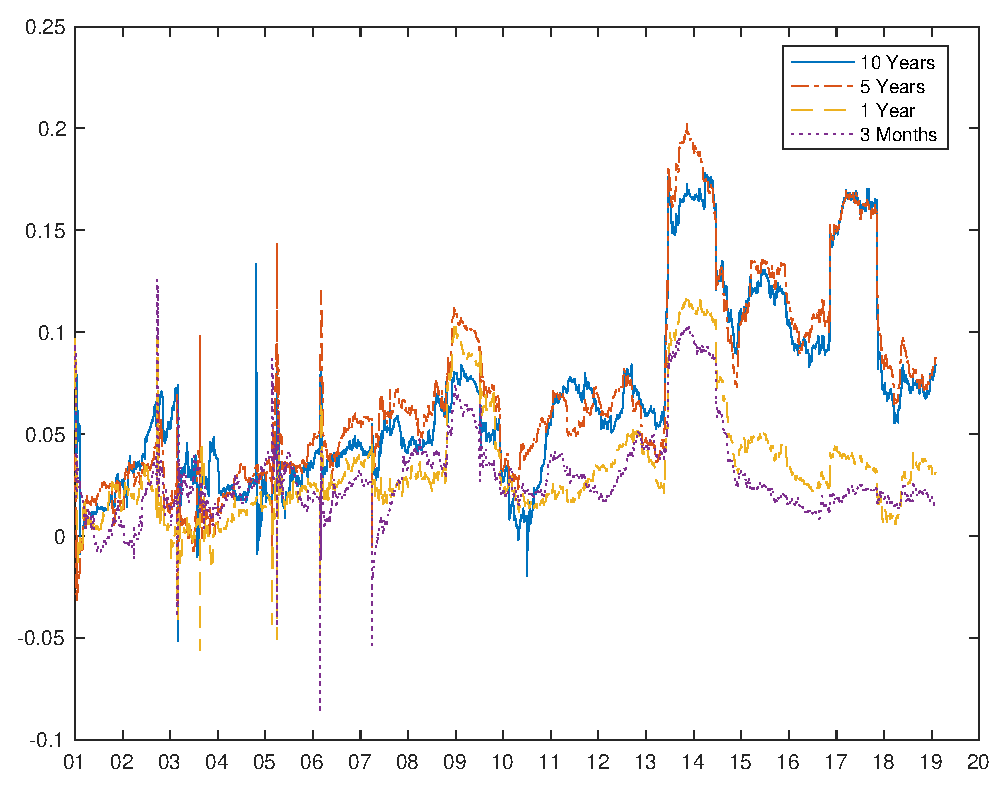
\includegraphics[trim={0cm 0cm 0cm 0cm},clip,height=0.38\textheight,width=\linewidth]{../Figures/Estimation/rolling_dn_data.eps} \\
						\vspace{-0.37cm}
						\caption{Emerging Markets} \label{subfig:rolling_tsEM}
						\vspace{0.4cm}
					\end{subfigure}
					
					\begin{subfigure}[t]{\linewidth}
						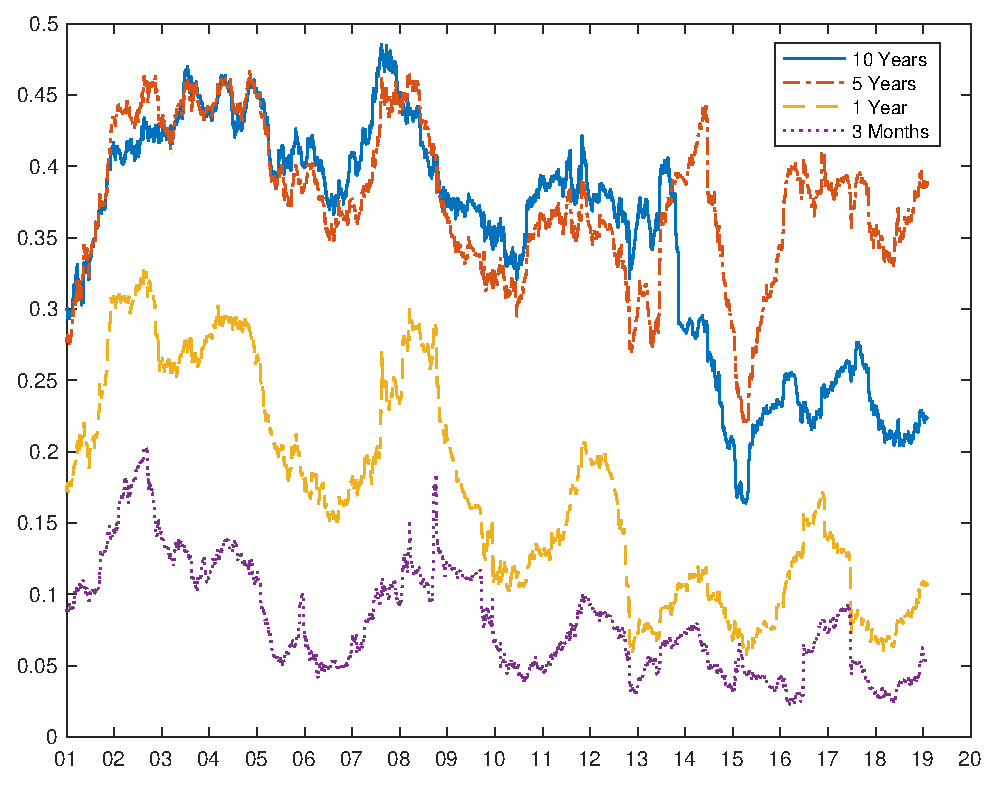
\includegraphics[trim={0cm 0cm 0cm 0cm},clip,height=0.38\textheight,width=\linewidth]{../Figures/Estimation/rolling_dn_data_AE.eps} \\
						\vspace{-0.37cm}
						\caption{Advanced Economies} \label{subfig:rolling_tsAE}
						\vspace{0.4cm}
					\end{subfigure}
					
				\end{center}
				\vspace{-0.45cm}
				\fignotes{This figure plots one-year rolling correlation coefficients of daily changes in the nominal yields of emerging markets	and advanced economies averaged across country pairs for the for 10-year (solid line), 5-year (dash-dotted line), 1-year (dashed line), and 3-month (dotted line) maturities.}
			\end{minipage}
		\end{center}
	\end{figure}
\end{document}
% trim = {<left> <lower> <right> <upper>}

The long-term yields of emerging markets are indeed more connected than short-term ones, although local factors remain relevant.
Figure \ref{subfig:rolling_tsEM} shows that the long-term yields of emerging markets became more connected after the global financial crisis, and more so since the taper tantrum episode of 2013. 
Meanwhile, according to figure \ref{subfig:rolling_tsAE}, the long-term yields of advanced economies have been more connected among themselves since the beginning of the sample period. 
On average, the correlation among the long-term yields of emerging markets is less than half that of the long-term yields of advanced economies, suggesting that local investors are relevant holders of medium- and long-term bonds issued by emerging markets. Indeed, even though the share of foreign investors in the LC bonds of emerging markets has increased over time (from 10\% in 2008 to 25\% in 2019 according to \cite{KolasaWesolowski:2020}), the next section shows that local factors are still important drivers for the long end of their yield curves.

\subsubsection{Drivers of Yields}
The yield curve channel requires one to distinguish between interest rates at different maturities and calls attention to the role of the U.S. term premium. 
This subsection assesses the role of the components of U.S. yields (the average expected future short rate and the term premium) in explaining the components of emerging market yields at different maturities. 
In fact, the assessment of the yield curve channel would be limited without the decomposition of U.S. and emerging market yields. 
For this purpose, I run the following panel regressions 
\begin{equation} \label{eq:nPanelDCMP}
	\eqpanelTPreg .
\end{equation}
\noindent in which \(\alpha_{\idxi}\) are country fixed effects, \(z^{1}_{\idxspnl}\) is a vector containing the components of the U.S. yield curve, \(z^{2}_{\idxspnl}\) is a vector of global and domestic variables that potentially drive emerging market yields, and \(u_{\idxspnl}\) is the error term. 
The dependent variable \(\yld_{\idxspnl}\) is either the nominal yield or any of its three components for both 10- and 2-year maturities.\footnote{ \cite{Kalemli-Ozcan:2019} focuses on yields with maturities of 1 year or less. Here, I focus on the 2-year yield because it is a benchmark commonly used by market participants. The conclusions based on the 10- and 2-year maturities carry over to the 5- and 1-year maturities, which are reported in appendix \ref{sec:AppTables}. The 1-year maturity is the shortest one for which the decomposition of U.S. yields used here is available.} 
As before, I use Driscoll--Kraay standard errors to test for significance.\footnote{ The Pesaran test of cross-sectional independence is rejected in all cases at the 1\% significance level.} 

The explanatory variables of interest are the components of U.S. yields, which come from the model of \cite{KimWright:2005}, who address the small sample problem using survey forecasts of future short rates. 
I control for the domestic monetary stance and local macroeconomic conditions by using the policy rate reported by each country to the Bank for International Settlements, as well as domestic inflation and unemployment rates. 
\cite{Rey:2013} highlights the role of the Cboe Volatility Index (VIX) as an important driver of the global financial cycle, which reflects the implied volatility in stock option prices and is usually seen as a measure of risk aversion and economic uncertainty.\footnote{ Given the sudden spikes in the index, it is common to use it in logs. For consistency, the other uncertainty indexes are also used in logs.}
\cite{BakerBloomDavis:2016} construct a news-based economic policy uncertainty (EPU) index that serves as the basis for the global and U.S. versions,\footnote{ Although the EPU index has been replicated for different countries, it is only available for five of the emerging markets in the sample: Brazil, Colombia, Mexico, Russia and South Korea.} which are used as alternative, and arguably exogenous, measures of global uncertainty.
The index of global economic activity proposed by \cite{Hamilton:2021} captures real variables. 
Finally, the exchange rate (LC per USD) is included to rule out explanations of changes in yields due to currency movements; the exchange rate is standardized for each country over the sample period.

Tables \ref{tab:ycdcmp10y} and \ref{tab:ycdcmp2y} report the results.\footnote{ The tables report the estimates for the full specification of the model. The results are robust to specifications of the model that progressively include the regressors for each dependent variable.} 
The evidence is in line with the yield curve channel. 
First, the response of the average expected future short rates of emerging markets to the domestic policy rate decreases with maturity and is positively associated with its U.S. counterpart only at the long end, both results are in line with the argument that monetary autonomy is stronger at the short end than at the long end of the curve. 
Second, the term premia in emerging markets are positively associated with the U.S. term premium and the VIX only at the long end, both results align with the claim that the global financial cycle (represented here by those two variables) is more relevant for the long end than for the short end of the curve \citep{Obstfeld:2015}. 
Third, the U.S. term premium not only influences the yields in emerging markets through its effect on their term premia, as suggested by \cite{Turner:2014}, but through the other components too. 
In particular, the influence on the average expected future short rates of emerging markets supports the risk spillovers mechanism highlighted by \cite{Kalemli-Ozcan:2019}, which can be directly tested thanks to the yield decompositions. 
Further, those risk spillovers are indeed stronger at the short end and operate through the U.S. term premium rather than the VIX. 
These conclusions would be different if the risk that emerging markets might default were to be ignored since the term premium and the credit risk components would be mixed together.

\documentclass[a4paper,12pt]{article}
\usepackage[labelsep=period,labelfont=bf]{caption}
\usepackage{multirow}
\usepackage{booktabs}
\usepackage{threeparttable}
\usepackage{pdflscape}
\usepackage{tabularx}
\usepackage[margin=1in]{geometry}
\input{../Settings/macros_global}		   % Personalized commands
%% Personalized Macros
% Variable Definitions, Equations

%-------------------------------------------------------------------
% Variable Definitions
%-------------------------------------------------------------------
\providecommand{\tnr}{n}
\providecommand{\tnrfwd}{m}
\providecommand{\idxt}{t}
\providecommand{\idxi}{i}
\providecommand{\idxh}{h}
\providecommand{\idxs}{\idxt,\tnr}
\providecommand{\idxsfwd}{\tnr | \tnrfwd}
\providecommand{\idxsfwdt}{\idxt,\idxsfwd}
\providecommand{\idxspnl}{\idxi,\idxt}
\providecommand{\idxspnlfwd}{\idxi,{\idxt+\idxh}}
\providecommand{\idxspnllag}{\idxi,{\idxt-1}}
\providecommand{\idxspnllaglag}{\idxi,{\idxt-j}}
\providecommand{\fInst}{f_{\idxs}}
\providecommand{\yld}{y}
\providecommand{\xpc}{e}
\providecommand{\yZero}{\yld_{\idxs}}
\providecommand{\yZeroQ}{\yZero^{\Qmeasure}}
\providecommand{\yZeroP}{\yZero^{\Pmeasure}}
\providecommand{\yZeroE}{\yZero^{\xpc}}
\providecommand{\yZeroFwd}{\frate_{\idxsfwdt}}
\providecommand{\yZeroEfwd}{\yZeroFwd^{\xpc}}
\providecommand{\Pzero}{P_{\idxs}}
\providecommand{\Pzerolag}{P_{\idxt+1,\tnr-1}}
\providecommand{\srate}{i}
\providecommand{\shortrate}{\srate_{\idxt}}
\providecommand{\shortratelag}{\srate_{\idxt-1}}
\providecommand{\frate}{f}
\providecommand{\realrate}{r_{\idxs}}
\providecommand{\rateSvy}{\srate_{\idxs}^{survey}}
\providecommand{\SDF}{M_{\idxt+1}}
\providecommand{\SDFprod}{\ExpP \left[\Pi_{j=1} ^\tnr M_{\idxt+j}\right]}
\providecommand{\SDFsum}{\ExpQ \left[\exp \left(- \Sigma_{j=0} ^{\tnr-1} \srate_{\idxt+j} \right) \right]}
\providecommand{\Xvars}{X_{\idxt}}
\providecommand{\XvarsFwd}{X_{\idxt+1}}
\providecommand{\affineA}{A_{\tnr}}
\providecommand{\affineB}{B_{\tnr}}
\providecommand{\affineAfwd}{A_{\tnr + 1}}
\providecommand{\affineBfwd}{B_{\tnr + 1}}
\providecommand{\affineAQ}{\affineA^{\Qmeasure}}
\providecommand{\affineBQ}{\affineB^{\Qmeasure}}
\providecommand{\affineAP}{\affineA^{\Pmeasure}}
\providecommand{\affineBP}{\affineB^{\Pmeasure}}
\providecommand{\affineAe}{\affineA^{\xpc}}
\providecommand{\affineBe}{\affineB^{\xpc}}
\providecommand{\affineAeFwd}{A_{\idxsfwd}^{\xpc}}
\providecommand{\affineBeFwd}{B_{\idxsfwd}^{\xpc}}
\providecommand{\yLCnom}{\yld_{\idxs} ^{LC}}
\providecommand{\yLCsynt}{\widetilde{\yld}_{\idxs} ^{LC}}
\providecommand{\yUS}{y_{\idxs} ^{US}}
\providecommand{\yUSsynt}{\widetilde{\yld}_{\idxs} ^{US}}
\providecommand{\fx}{\mathit{s}}

% Math fonts
\providecommand{\Xdim}{\mathrm{K}}
\providecommand{\Ydim}{\mathrm{N}}
\providecommand{\Sdim}{\mathrm{S}}
\providecommand{\Normal}{\mathcal{N}}
\providecommand{\Pmeasure}{\mathbb{P}}
\providecommand{\Qmeasure}{\mathbb{Q}}
\providecommand{\Expec}{\mathrm{E}_{t}}
\providecommand{\ExpP}{\mathrm{E}^{\Pmeasure}_{t}}
\providecommand{\ExpQ}{\mathrm{E}^{\Qmeasure}_{t}}
\providecommand{\Svy}{S}
\providecommand{\yVec}{\mathbf{\yld}_{t}}
\providecommand{\ySVec}{\yVec^{\Svy}}
\providecommand{\Avec}{\mathbf{A}}
\providecommand{\Bvec}{\mathbf{B}}
\providecommand{\ASvec}{\mathbf{A}^{\Svy}}
\providecommand{\BSvec}{\mathbf{B}^{\Svy}}
\providecommand{\uVec}{\mathbf{u}_{t}}
\providecommand{\uSVec}{\mathbf{u}_{t}^{\Svy}}
\providecommand{\Svec}{\mathbf{\Sigma}}
\providecommand{\SyVec}{\mathbf{\Svec}_{Y}}
\providecommand{\SsVec}{\mathbf{\Svec}_{\Svy}}

% Greeks
\providecommand{\termprm}{\tau_{\idxs}}
\providecommand{\riskprice}{\lambda_{t}}
\providecommand{\lambdazero}{\lambda_{0}}
\providecommand{\lambdaone}{\lambda_{1}}
\providecommand{\fwdprm}{\rho_{\idxs}}
\providecommand{\CIPdev}{\phi_{\idxs}}
\providecommand{\deltazero}{\delta_{0}}
\providecommand{\deltaone}{\delta_{1}}
\providecommand{\error}{\nu_{t+1}}
\providecommand{\errorQ}{\error^{\Qmeasure}}
\providecommand{\errorP}{\error^{\Pmeasure}}
\providecommand{\XmuP}{\mu^{\Pmeasure}}
\providecommand{\XmuQ}{\mu^{\Qmeasure}}
\providecommand{\XSigma}{\Sigma}
\providecommand{\XPhiP}{\Phi^{\Pmeasure}}
\providecommand{\XPhiQ}{\Phi^{\Qmeasure}}
\providecommand{\betaLT}{\beta_{0}}
\providecommand{\betaST}{\beta_{1}}
\providecommand{\betaMTns}{\beta_{2}}
\providecommand{\betaMTnss}{\beta_{3}}
\providecommand{\tauNS}{\tau_{1}}
\providecommand{\tauNSS}{\tau_{2}}
\providecommand{\tnrTauNS}{\tnr/\tauNS}
\providecommand{\tnrTauNSS}{\tnr/\tauNSS}
\providecommand{\params}{\theta}
\providecommand{\Vasy}{\Omega}
\providecommand{\cmpnt}{\Psi}
\providecommand{\Jacobian}{\Gamma}
\providecommand{\Hessian}{\mathcal{H}_\params}
\providecommand{\asydstr}{\sqrt{\Ydim} \left( \widehat{\cmpnt} - \cmpnt \right) \xrightarrow[]{d} \Normal \left(0,\, \Jacobian \, \Vasy \, \Jacobian' \right)}
\providecommand{\sampleHjoint}{\frac{1}{\Ydim} \frac{\partial^{2} \ell_{\Ydim} (\widehat{\params})}{\partial \params \partial \params'}}
\providecommand{\sampleHindiv}{\frac{1}{\Ydim} \sum_{i = 1}^{\Ydim} \frac{\partial^{2} \log \mathit{f} (X_{i} | \widehat{\params})}{\partial \params \partial \params'}}

% Nelson-Siegel_Svensson
\providecommand{\loadSTnsFwd}{\exp\left(-\tnrTauNS \right)}
\providecommand{\loadSTnssFwd}{\exp\left(-\tnrTauNSS \right)}
\providecommand{\loadMTnsFwd}{\left(\tnrTauNS\right) \loadSTnsFwd}
\providecommand{\loadMTnssFwd}{\left(\tnrTauNSS\right) \loadSTnssFwd}
\providecommand{\loadSTnsZero}{\frac{1-\loadSTnsFwd}{\tnrTauNS}}
\providecommand{\loadSTnssZero}{\frac{1-\loadSTnssFwd}{\tnrTauNSS}}
\providecommand{\loadMTnsZero}{\left(\loadSTnsZero - \loadSTnsFwd \right)}
\providecommand{\loadMTnssZero}{\left( \loadSTnssZero - \loadSTnssFwd \right)}

% DELETE in a later revision
\providecommand{\Xmu}{\mu}
\providecommand{\XPhi}{\Phi}
\providecommand{\XmuStar}{\mu^{*}}
\providecommand{\XPhiStar}{\Phi^{*}}
\providecommand{\STrate}{r}
\providecommand{\rShort}{\STrate_{t}}
\providecommand{\rShortlag}{\STrate_{t-1}}
\providecommand{\ySvy}{\STrate_{\idxs}^{survey}}
\providecommand{\TPatsm}{tp_{\idxs}}

%-------------------------------------------------------------------
% Equations
%-------------------------------------------------------------------
\newcommand{\eqyLCsynt}{\yLCsynt = \yUS + \fwdprm}
\newcommand{\eqCIPdevDS}{\CIPdev = \yLCnom - \yLCsynt}
\newcommand{\eqCIPdevQ}{\CIPdev = \yLCnom - \yZeroQ}

\newcommand{\PzeroP}{\Pzero = \ExpP \left[ \SDF \Pzerolag \right]}
\newcommand{\PzeroQ}{\Pzero = \ExpQ \left[ \exp\left(- \shortrate\right) \Pzerolag \right]}

\newcommand{\eqXvarsFwdQ}{\XvarsFwd = \XmuQ + \XPhiQ \Xvars  + \XSigma \errorQ}
\newcommand{\eqshortrate}{\shortrate = \deltazero + \deltaone' \Xvars}
\newcommand{\eqyZeroP}{\yZeroP = \affineAP + \affineBP \Xvars}
\newcommand{\eqyZeroQ}{\yZeroQ = \affineAQ + \affineBQ \Xvars}
\newcommand{\eqTP}{\termprm = \yZeroQ - \yZeroP}
\newcommand{\eqXvarsFwdP}{\XvarsFwd = \XmuP + \XPhiP \Xvars  + \XSigma \errorP}
\newcommand{\eqriskprice}{\riskprice = \lambdazero + \lambdaone \Xvars}
\newcommand{\eqSDF}{\SDF = \exp\left( -\shortrate -\frac{1}{2} \riskprice' \riskprice - \riskprice' \errorP \right)}

\newcommand{\eqpanelUCSV}{\tau_{\idxspnl} = \alpha_{\idxi} + \beta_{1} \sigma^{\pi}_{\idxspnl} + \beta_{2} GDP_{\idxspnl} + u_{\idxspnl}}
\newcommand{\eqpanelTPreg}{\yld_{\idxspnl} = \alpha_{\idxi} + \gamma_{1}' z^{1}_{\idxspnl} + \gamma_{2}' z^{2}_{\idxspnl} + u_{\idxspnl}}
\newcommand{\eqySvy}{\rateSvy = \frac{\widehat{\beta}_{0}}{1-\widehat{\beta}_{\srate}} + \frac{\widehat{\beta}_{{\pi}}}{1-\widehat{\beta}_{\srate}} \pi_{\idxs}^{survey} + \frac{\widehat{\beta}_{{g}}}{1-\widehat{\beta}_{\srate}} g_{\idxs}^{survey} }

\newcommand{\eqyFwd}{\yZeroFwd = \left( \tnrfwd \yld_{\idxt,\tnrfwd} - \tnr \yZero \right)/ \left( \tnrfwd - \tnr \right) }
\newcommand{\eqAeFwd}{\affineAeFwd = \left( \tnrfwd A_{\tnrfwd}^{\xpc}  - \tnr \affineAe \right)/ \left( \tnrfwd - \tnr \right) }
\newcommand{\eqBeFwd}{\affineBeFwd = \left( \tnrfwd B_{\tnrfwd}^{\xpc}  - \tnr \affineBe \right)/ \left( \tnrfwd - \tnr \right) }
\newcommand{\eqrrt}{\rateSvy = \realrate^{*} + \pi^{e}_{\idxs} = \left( \srate^{SPF survey}_{\idxs} - \pi^{SPF survey}_{\idxs} \right) + \fwdprm^{\perp} + \pi^{CE survey}_{\idxs} }


\newcommand{\eqyVecY}{\yVec = \Avec + \Bvec \Xvars + \SyVec \uVec}
\newcommand{\eqyVecS}{\ySVec = \ASvec + \BSvec \Xvars + \SsVec \uSVec}

% One shock at a time
%\newcommand{\eqpanelLP}{\yld_{\idxspnlfwd} - \yld_{\idxspnllag} = \alpha_{\idxh,\idxi} + \beta_{\idxh} \epsilon_{\idxt} + \gamma_{\idxh} \Delta \yld_{\idxspnllag} + \phi_{\idxh} \fx_{\idxspnllag}  + u_{\idxspnlfwd}}

% All shocks at once
\newcommand{\eqpanelLP}{\yld_{\idxspnlfwd} - \yld_{\idxspnllag} = \alpha_{\idxh,\idxi} + \sum^{3}_{j = 1} \beta^{j}_{\idxh} \epsilon^{j}_{\idxt} + \gamma_{\idxh} \Delta \yld_{\idxspnllag} + \eta_{\idxh} \fx_{\idxspnllag}  + u_{\idxspnlfwd}} 

\newcommand{\eqpanelLPlevels}{\yld_{\idxspnlfwd} = \alpha_{\idxh,\idxi} + \sum^{3}_{j = 1} \beta^{j}_{\idxh} \epsilon^{j}_{\idxt} + \sum^{2}_{j = 1} \gamma^{j}_{\idxh} \yld_{\idxspnllaglag} + \eta_{\idxh} \fx_{\idxspnllag}  + u_{\idxspnlfwd}} 
% \beta^{target}_{\idxh} \epsilon^{target}_{\idxt} + \beta^{path}_{\idxh} \epsilon^{path}_{\idxt} + \beta^{lsap}_{\idxh} \epsilon^{lsap}_{\idxt} 
			% Personalized commands
\pagestyle{empty}

\begin{document}
	\begin{normalsize}
%		\begin{landscape}
			\begin{table}
				\begin{center}
					\caption{Drivers of the Emerging Market 10-Year Nominal Yield and Its Components} \label{tab:ycdcmp10y}
					\begin{threeparttable}
						\estauto{../Tables/f_ycdcmp10y.tex}{6}
						\tabnote{This table reports the estimated slope coefficients of panel data regressions of the 10-year nominal yield and its components (expected short rate, term premium and credit risk compensation) on selected explanatory variables. The sample includes monthly data for 15 emerging markets starting in 2000:1 and ending in 2021:7. The dependent variables are expressed in basis points. The explanatory variables are the U.S. term premium and the U.S. expected short rate according to \cite{KimWright:2005} with the same maturity as the dependent variables, the policy rate, domestic inflation and unemployment, the standardized exchange rate (local currency per USD), the log of the VIX, the log of the U.S. and global economic policy uncertainty indexes based on \cite{BakerBloomDavis:2016}, the global economic activity index of \cite{Hamilton:2021}. Driscoll--Kraay standard errors in parenthesis. The lag length up to which the residuals may be autocorrelated is indicated. *, **, *** asterisks respectively indicate significance at the 10\%, 5\% and 1\% level.}
					\end{threeparttable}
				\end{center}
			\end{table}
%		\end{landscape}
	\end{normalsize}
\end{document}

\documentclass[a4paper,12pt]{article}
\usepackage[labelsep=period,labelfont=bf]{caption}
\usepackage{multirow}
\usepackage{booktabs}
\usepackage{threeparttable}
\usepackage{pdflscape}
\usepackage{tabularx}
%\usepackage[margin=1in]{geometry}
%%% Personalized Macros
% Definitions, Equations, Table of Contents, Tables, Subcaptions, Paths, Text Fomats

%-------------------------------------------------------------------
% Variable Definitions
%-------------------------------------------------------------------
\providecommand{\tnr}{n}
\providecommand{\tnrfwd}{m}
\providecommand{\idxt}{t}
\providecommand{\idxi}{i}
\providecommand{\idxh}{h}
\providecommand{\idxs}{\idxt,\tnr}
\providecommand{\idxsfwd}{\tnr | \tnrfwd}
\providecommand{\idxsfwdt}{\idxt,\idxsfwd}
\providecommand{\idxspnl}{\idxi,\idxt}
\providecommand{\idxspnlfwd}{\idxi,{\idxt+\idxh}}
\providecommand{\idxspnllag}{\idxi,{\idxt-1}}
\providecommand{\idxspnllaglag}{\idxi,{\idxt-j}}
\providecommand{\fInst}{f_{\idxs}}
\providecommand{\yld}{y}
\providecommand{\xpc}{e}
\providecommand{\yZero}{\yld_{\idxs}}
\providecommand{\yZeroQ}{\yZero^{\Qmeasure}}
\providecommand{\yZeroP}{\yZero^{\Pmeasure}}
\providecommand{\yZeroE}{\yZero^{\xpc}}
\providecommand{\yZeroFwd}{\frate_{\idxsfwdt}}
\providecommand{\yZeroEfwd}{\yZeroFwd^{\xpc}}
\providecommand{\Pzero}{P_{\idxs}}
\providecommand{\Pzerolag}{P_{\idxt+1,\tnr-1}}
\providecommand{\srate}{i}
\providecommand{\shortrate}{\srate_{\idxt}}
\providecommand{\shortratelag}{\srate_{\idxt-1}}
\providecommand{\frate}{f}
\providecommand{\realrate}{r_{\idxs}}
\providecommand{\rateSvy}{\srate_{\idxs}^{survey}}
\providecommand{\SDF}{M_{\idxt+1}}
\providecommand{\SDFprod}{\ExpP \left[\Pi_{j=1} ^\tnr M_{\idxt+j}\right]}
\providecommand{\SDFsum}{\ExpQ \left[\exp \left(- \Sigma_{j=0} ^{\tnr-1} \srate_{\idxt+j} \right) \right]}
\providecommand{\Xvars}{X_{\idxt}}
\providecommand{\XvarsFwd}{X_{\idxt+1}}
\providecommand{\affineA}{A_{\tnr}}
\providecommand{\affineB}{B_{\tnr}}
\providecommand{\affineAfwd}{A_{\tnr + 1}}
\providecommand{\affineBfwd}{B_{\tnr + 1}}
\providecommand{\affineAQ}{\affineA^{\Qmeasure}}
\providecommand{\affineBQ}{\affineB^{\Qmeasure}}
\providecommand{\affineAP}{\affineA^{\Pmeasure}}
\providecommand{\affineBP}{\affineB^{\Pmeasure}}
\providecommand{\affineAe}{\affineA^{\xpc}}
\providecommand{\affineBe}{\affineB^{\xpc}}
\providecommand{\affineAeFwd}{A_{\idxsfwd}^{\xpc}}
\providecommand{\affineBeFwd}{B_{\idxsfwd}^{\xpc}}
\providecommand{\yLCnom}{\yld_{\idxs} ^{LC}}
\providecommand{\yLCsynt}{\widetilde{\yld}_{\idxs} ^{LC}}
\providecommand{\yUS}{y_{\idxs} ^{US}}
\providecommand{\yUSsynt}{\widetilde{\yld}_{\idxs} ^{US}}
\providecommand{\fx}{\mathit{s}}

% Math fonts
\providecommand{\Xdim}{\mathrm{K}}
\providecommand{\Ydim}{\mathrm{N}}
\providecommand{\Sdim}{\mathrm{S}}
\providecommand{\Normal}{\mathcal{N}}
\providecommand{\Pmeasure}{\mathbb{P}}
\providecommand{\Qmeasure}{\mathbb{Q}}
\providecommand{\Expec}{\mathrm{E}_{t}}
\providecommand{\ExpP}{\mathrm{E}^{\Pmeasure}_{t}}
\providecommand{\ExpQ}{\mathrm{E}^{\Qmeasure}_{t}}
\providecommand{\Svy}{S}
\providecommand{\yVec}{\mathbf{\yld}_{t}}
\providecommand{\ySVec}{\yVec^{\Svy}}
\providecommand{\Avec}{\mathbf{A}}
\providecommand{\Bvec}{\mathbf{B}}
\providecommand{\ASvec}{\mathbf{A}^{\Svy}}
\providecommand{\BSvec}{\mathbf{B}^{\Svy}}
\providecommand{\uVec}{\mathbf{u}_{t}}
\providecommand{\uSVec}{\mathbf{u}_{t}^{\Svy}}
\providecommand{\Svec}{\mathbf{\Sigma}}
\providecommand{\SyVec}{\mathbf{\Svec}_{Y}}
\providecommand{\SsVec}{\mathbf{\Svec}_{\Svy}}

% Greeks
\providecommand{\termprm}{\tau_{\idxs}}
\providecommand{\riskprice}{\lambda_{t}}
\providecommand{\lambdazero}{\lambda_{0}}
\providecommand{\lambdaone}{\lambda_{1}}
\providecommand{\fwdprm}{\rho_{\idxs}}
\providecommand{\CIPdev}{\phi_{\idxs}}
\providecommand{\deltazero}{\delta_{0}}
\providecommand{\deltaone}{\delta_{1}}
\providecommand{\error}{\nu_{t+1}}
\providecommand{\errorQ}{\error^{\Qmeasure}}
\providecommand{\errorP}{\error^{\Pmeasure}}
\providecommand{\XmuP}{\mu^{\Pmeasure}}
\providecommand{\XmuQ}{\mu^{\Qmeasure}}
\providecommand{\XSigma}{\Sigma}
\providecommand{\XPhiP}{\Phi^{\Pmeasure}}
\providecommand{\XPhiQ}{\Phi^{\Qmeasure}}
\providecommand{\betaLT}{\beta_{0}}
\providecommand{\betaST}{\beta_{1}}
\providecommand{\betaMTns}{\beta_{2}}
\providecommand{\betaMTnss}{\beta_{3}}
\providecommand{\tauNS}{\tau_{1}}
\providecommand{\tauNSS}{\tau_{2}}
\providecommand{\tnrTauNS}{\tnr/\tauNS}
\providecommand{\tnrTauNSS}{\tnr/\tauNSS}
\providecommand{\params}{\theta}
\providecommand{\Vasy}{\Omega}
\providecommand{\cmpnt}{\Psi}
\providecommand{\Jacobian}{\Gamma}
\providecommand{\Hessian}{\mathcal{H}_\params}
\providecommand{\asydstr}{\sqrt{\Ydim} \left( \widehat{\cmpnt} - \cmpnt \right) \xrightarrow[]{d} \Normal \left(0,\, \Jacobian \, \Vasy \, \Jacobian' \right)}
\providecommand{\sampleHjoint}{\frac{1}{\Ydim} \frac{\partial^{2} \ell_{\Ydim} (\widehat{\params})}{\partial \params \partial \params'}}
\providecommand{\sampleHindiv}{\frac{1}{\Ydim} \sum_{i = 1}^{\Ydim} \frac{\partial^{2} \log \mathit{f} (X_{i} | \widehat{\params})}{\partial \params \partial \params'}}

% Nelson-Siegel_Svensson
\providecommand{\loadSTnsFwd}{\exp\left(-\tnrTauNS \right)}
\providecommand{\loadSTnssFwd}{\exp\left(-\tnrTauNSS \right)}
\providecommand{\loadMTnsFwd}{\left(\tnrTauNS\right) \loadSTnsFwd}
\providecommand{\loadMTnssFwd}{\left(\tnrTauNSS\right) \loadSTnssFwd}
\providecommand{\loadSTnsZero}{\frac{1-\loadSTnsFwd}{\tnrTauNS}}
\providecommand{\loadSTnssZero}{\frac{1-\loadSTnssFwd}{\tnrTauNSS}}
\providecommand{\loadMTnsZero}{\left(\loadSTnsZero - \loadSTnsFwd \right)}
\providecommand{\loadMTnssZero}{\left( \loadSTnssZero - \loadSTnssFwd \right)}

%\providecommand{\}{}
% DELETE in a later revision
\providecommand{\Xmu}{\mu}
\providecommand{\XPhi}{\Phi}
\providecommand{\XmuStar}{\mu^{*}}
\providecommand{\XPhiStar}{\Phi^{*}}
\providecommand{\STrate}{r}
\providecommand{\rShort}{\STrate_{t}}
\providecommand{\rShortlag}{\STrate_{t-1}}
\providecommand{\ySvy}{\STrate_{\idxs}^{survey}}
\providecommand{\TPatsm}{tp_{\idxs}}

%-------------------------------------------------------------------
% Equations
%-------------------------------------------------------------------
\newcommand{\eqyLCsynt}{\yLCsynt = \yUS + \fwdprm}
\newcommand{\eqCIPdevDS}{\CIPdev = \yLCnom - \yLCsynt}
\newcommand{\eqCIPdevQ}{\CIPdev = \yLCnom - \yZeroQ}

\newcommand{\PzeroP}{\Pzero = \ExpP \left[ \SDF \Pzerolag \right]}
\newcommand{\PzeroQ}{\Pzero = \ExpQ \left[ \exp\left(- \shortrate\right) \Pzerolag \right]}

\newcommand{\eqXvarsFwdQ}{\XvarsFwd = \XmuQ + \XPhiQ \Xvars  + \XSigma \errorQ}
\newcommand{\eqshortrate}{\shortrate = \deltazero + \deltaone' \Xvars}
\newcommand{\eqyZeroP}{\yZeroP = \affineAP + \affineBP \Xvars}
\newcommand{\eqyZeroQ}{\yZeroQ = \affineAQ + \affineBQ \Xvars}
\newcommand{\eqTP}{\termprm = \yZeroQ - \yZeroP}
\newcommand{\eqXvarsFwdP}{\XvarsFwd = \XmuP + \XPhiP \Xvars  + \XSigma \errorP}
\newcommand{\eqriskprice}{\riskprice = \lambdazero + \lambdaone \Xvars}
\newcommand{\eqSDF}{\SDF = \exp\left( -\shortrate -\frac{1}{2} \riskprice' \riskprice - \riskprice' \errorP \right)}
%\newcommand{}{}

\newcommand{\eqpanelUCSV}{\tau_{\idxspnl} = \alpha_{\idxi} + \beta_{1} \sigma^{\pi}_{\idxspnl} + \beta_{2} GDP_{\idxspnl} + u_{\idxspnl}}
\newcommand{\eqpanelTPreg}{\yld_{\idxspnl} = \alpha_{\idxi} + \gamma_{1}' z^{1}_{\idxspnl} + \gamma_{2}' z^{2}_{\idxspnl} + u_{\idxspnl}}
\newcommand{\eqySvy}{\rateSvy = \frac{\widehat{\beta}_{0}}{1-\widehat{\beta}_{\srate}} + \frac{\widehat{\beta}_{{\pi}}}{1-\widehat{\beta}_{\srate}} \pi_{\idxs}^{survey} + \frac{\widehat{\beta}_{{g}}}{1-\widehat{\beta}_{\srate}} g_{\idxs}^{survey} }

\newcommand{\eqyFwd}{\yZeroFwd = \left( \tnrfwd \yld_{\idxt,\tnrfwd} - \tnr \yZero \right)/ \left( \tnrfwd - \tnr \right) }
\newcommand{\eqAeFwd}{\affineAeFwd = \left( \tnrfwd A_{\tnrfwd}^{\xpc}  - \tnr \affineAe \right)/ \left( \tnrfwd - \tnr \right) }
\newcommand{\eqBeFwd}{\affineAeFwd = \left( \tnrfwd B_{\tnrfwd}^{\xpc}  - \tnr \affineBe \right)/ \left( \tnrfwd - \tnr \right) }
\newcommand{\eqrrt}{\rateSvy = \realrate^{*} + \pi^{e}_{\idxs} = \left( \srate^{SPF survey}_{\idxs} - \pi^{SPF survey}_{\idxs} \right) + \fwdprm^{\perp} + \pi^{CE survey}_{\idxs} }


\newcommand{\eqyVecY}{\yVec = \Avec + \Bvec \Xvars + \SyVec \uVec}
\newcommand{\eqyVecS}{\ySVec = \ASvec + \BSvec \Xvars + \SsVec \uSVec}

% One shock at a time
%\newcommand{\eqpanelLP}{\yld_{\idxspnlfwd} - \yld_{\idxspnllag} = \alpha_{\idxh,\idxi} + \beta_{\idxh} \epsilon_{\idxt} + \gamma_{\idxh} \Delta \yld_{\idxspnllag} + \phi_{\idxh} \fx_{\idxspnllag}  + u_{\idxspnlfwd}}

% All shocks at once
\newcommand{\eqpanelLP}{\yld_{\idxspnlfwd} - \yld_{\idxspnllag} = \alpha_{\idxh,\idxi} + \sum^{3}_{j = 1} \beta^{j}_{\idxh} \epsilon^{j}_{\idxt} + \gamma_{\idxh} \Delta \yld_{\idxspnllag} + \eta_{\idxh} \fx_{\idxspnllag}  + u_{\idxspnlfwd}} 

\newcommand{\eqpanelLPlevels}{\yld_{\idxspnlfwd} = \alpha_{\idxh,\idxi} + \sum^{3}_{j = 1} \beta^{j}_{\idxh} \epsilon^{j}_{\idxt} + \sum^{2}_{j = 1} \gamma^{j}_{\idxh} \yld_{\idxspnllaglag} + \eta_{\idxh} \fx_{\idxspnllag}  + u_{\idxspnlfwd}} 
% \beta^{target}_{\idxh} \epsilon^{target}_{\idxt} + \beta^{path}_{\idxh} \epsilon^{path}_{\idxt} + \beta^{lsap}_{\idxh} \epsilon^{lsap}_{\idxt} 

%---------------------------------------------------------------
% Table of Contents
%---------------------------------------------------------------
% Link to ToC from section
\newcommand{\gototoc}{\vspace{-2cm} \null\hfill [\hyperlink{toc}{Go2ToC}] \newline}

% Link back to section from ToC
\newcommand{\maketoc}{
	\hypertarget{toc}{}
	\newpage
	\tableofcontents
	\vspace{2.5\bigskipamount} }

% Box with bullets for tasks to do in a section
\newenvironment{boxeditems}
	{\begin{tabular}{|p{\linewidth}|}
	\hline
	\begin{itemize}
	}
	{
	\end{itemize}
	\\ \hline
	\end{tabular} \\
	}

%---------------------------------------------------------------
% Tables: Estout Commands following Jörg Weber
%---------------------------------------------------------------
\newcommand{\sym}[1]{\rlap{#1}}

\let\estinput=\input	% define new input command to flatten the document

\newcommand{\estauto}[2]{
	\newcolumntype{C}{>{\centering\arraybackslash}X}
	\vspace{.75ex}{
%		\begin{tabularx}{1.4\textwidth}{l*{#2}C}
		\begin{tabularx}{0.95\linewidth}{l*{#2}C}
			\toprule
			\estinput{#1}
			\\ \bottomrule
			\addlinespace[.75ex]
		\end{tabularx}
	}
}

% Allow line breaks with \\ in specialcells
\newcommand{\specialcell}[2][c]{\begin{tabular}[#1]{@{}c@{}}#2\end{tabular}}

%---------------------------------------------------------------
% Subcaptions
%---------------------------------------------------------------
% Notes after figures following Jörg Weber
\newcommand{\figtext}[1]{
	\vspace{-1ex}
	\captionsetup{justification=justified,font=footnotesize}
	\caption*{#1}
%	\captionsetup{justification=raggedright,singlelinecheck=false,font=footnotesize}
%	\caption*{\hspace{6pt}\hangindent=1.5em #1}
}

\newcommand{\fignote}[1]{\figtext{\emph{Note:~}~#1}}
\newcommand{\fignotes}[1]{\figtext{\emph{Notes:~}~#1}}

% Notes after tables
\newcommand{\tabnote}[1]{
	\begin{tablenotes}[para,flushleft]
		\footnotesize \emph{Notes:~}~#1
	\end{tablenotes}
}

%---------------------------------------------------------------
% Paths
%---------------------------------------------------------------
%\newcommand*{\pathFigs}{../Figures}
%\input{pathFigs/fig1.tex}

%---------------------------------------------------------------
% Text Fomats
%---------------------------------------------------------------
%\newcommand{\txtbi}[1]{\textbf{\textit{#1}}}

%---------------------------------------------------------------
% Other
%---------------------------------------------------------------
%\newcommand\LL[1]{\multicolumn{2}{|l}{#1}}
%\newcommand\RR[1]{\multicolumn{2}{c|}{#1}}
%\newcommand\LR[1]{\multicolumn{2}{|c|}{#1}}
%\newcommand\LL[1]{\multicolumn{1}{|c}{#1}}
%\newcommand\RR[1]{\multicolumn{1}{c|}{#1}}
%\newcommand\LR[1]{\multicolumn{1}{|c|}{#1}}

\begin{document}
	\begin{normalsize}
%		\begin{landscape}
			\begin{table}
				\begin{center}
					\caption{Drivers of the 2-Year Nominal Yield and Its Components} \label{tab:ycdcmp2y}
					\begin{threeparttable}
						\estauto{../Tables/f_ycdcmp2y.tex}{6}
						\tabnote{This table reports the estimated slope coefficients of panel data regressions of the 2-year nominal yields and their components on selected explanatory variables. The sample includes monthly data for 15 countries starting in 2000:1 and ending in 2019:12. The dependent variables are the nominal (Nominal) and synthetic (Synth.) yields, the expected short rate (ESR), the term premium (TP), the credit risk premium (CRP) and the forward premium (FP). All dependent variables are expressed in basis points. The explanatory variables are the U.S. expected short rate (US ER), the U.S. term premium (US TP), the log of the Vix, the global EPU index (EPU), the industrial production-based global activity index (Global IP), inflation, unemployment and the monthly returns in the Standard \& Poor's stock market index (S\&P), the price of oil for the WTI benchmark (Oil) and the exchange rate (FX). All cases include country fixed effects. Heteroskedasticity and autocorrelation consistent standard errors are in parenthesis. *, **, *** asterisks respectively indicate significance at the 10\%, 5\% and 1\% level.}
					\end{threeparttable}
				\end{center}
			\end{table}
%		\end{landscape}
	\end{normalsize}
\end{document}

A glimpse on the drivers of the yields of emerging markets is a byproduct of the analysis on the yield curve channel. 
For instance, inflation and unemployment are key domestic variables. 
In particular, the term premium and the credit risk compensation are countercyclical, investors demand higher compensations during recessions, when the unemployment rate increases. 
Moreover, the positive association between inflation and the term premium conforms with the idea that inflation erodes the value of nominal bonds and so, in periods of rising inflation investors demand a higher term premium. 
As expected for measures of risk and uncertainty, shifts in the VIX are positively associated with the term premium (at the long end) and the credit risk compensation. %, but not with the expected future short rate.
Also, higher global economic uncertainty induces a flight to quality, whereas higher U.S. economic uncertainty leads to a reduction in the perceived credit quality.\footnote{ The coefficient for the EPU global index in the expected short rate column is negative, while the coefficient for the U.S. EPU index in the credit risk compensation column is positive.}
Lastly, there is evidence supporting the risk-taking channel of exchange rates,\footnote{ According to the standard trade-channel effect, an appreciation is contractionary because it discourages exports and stimulates imports, reducing the trade balance.} 
according to which a currency appreciation is associated with easier financial conditions (and compressed sovereign bond spreads) due to balance sheet effects.
However, here it works through the expected future short rate and the term premium rather than through the credit risk compensation as reported by \cite{HofmannShimShin:2020}.

Thus far, the measures of comovement reported above %in section \ref{sec:Comovement} 
are unconditional, so not specifically driven by monetary policy surprises. At the same time, the yield decompositions have been valuable to assess the validity of the yield curve channel and understand the driving forces behind the sovereign yields of emerging markets, but the specification in equation (\ref{eq:nPanelDCMP}) may suffer from econometric problems such as persistent variables, reverse causality and omitted variables. These issues are addressed next.


\subsection{Identification of Monetary Policy Surprises} \label{sec:USMPS}
\iftoggle{toclinks}{\gototoc}{} % Turn it on/off in packages.tex, command in macros.tex

Surprises in monetary policy decisions are identified using intraday data on asset prices around Fed's monetary policy announcements in order to capture changes in the information set of market participants. 
Asset price changes are calculated from 15 minutes before to 1 hour and 45 minutes after each Federal Open Market Committee (FOMC) meeting between January 2000 and March 2019 giving a total of 163 events;\footnote{ Following \cite{GSS:2005a}, I exclude the meeting of September 2001.} neither minute releases nor speeches by Fed officials are included. 
The surprises are set to zero in non-announcement days. 

\cite{GSS:2005a} and \cite{Swanson:2021} show that U.S. monetary policy has more than one dimension, meaning that asset prices respond to different types of news about monetary policy. 
Following \cite{RogersScottiWright:2018}, I consider three separate types of U.S. monetary policy surprises, referred to hereinafter as target, forward guidance and asset purchase surprises. 
Target surprises are equal to the change in the yield on the current- or next-month federal funds futures contracts, as proposed by \cite{Kuttner:2001}. 
Forward guidance surprises are equal to the residual from regressing the yield change for the 8-quarters ahead Eurodollar futures contract onto the target surprise.\footnote{ The 4-quarters ahead Eurodollar futures contract could also be used, but intraday changes in that contract were essentially zero after 2011 since market participants expected no change in the policy rate for at least a year. Eurodollar futures contracts are bets on the future level of 3-month interest rates.} 
Asset purchase surprises are equal to the residual from regressing the yield change in the 10-year Treasury futures contract onto the target and forward guidance surprises. 
By construction, the three types of surprises are uncorrelated. 
Positive values in any of the surprises represent a tightening of the monetary policy stance, and vice versa.

The relevance of the surprises has varied over time. 
After 2008, there were no changes in the current policy rate until December 2015, so target surprises were essentially zero during that period. 
Meanwhile, asset purchase surprises are considered starting in October 2008 because their meaning is unclear before that date. 
Forward guidance surprises have nevertheless been relevant before and after the global financial crisis. 
Table \ref{tab:mpsstats} in the appendix reports descriptive statistics for the three types of surprises. 
In general, easing surprises are larger on average and more common than tightening surprises, which means that the Fed has been more aggressive in stimulating than in contracting the U.S. economy.


\subsection{The Effects on Emerging Market Yields} \label{sec:LPs} 
\iftoggle{toclinks}{\gototoc}{} % Turn it on/off in packages.tex, command in macros.tex

The transmission of U.S. monetary policy to the yields of emerging markets is assessed using panel local projections for the daily changes in the yields.\footnote{\cite{Jorda:2005} advocates the use of local projections as an alternative to VAR models in order to generate impulse responses that are robust to misspecification. See \cite{ACDM:2019} and \cite{HofmannShimShin:2020} for recent applications of panel local projections on related issues.} 
While event studies report the response of the variables on the day of a surprise, local projections additionally provide the responses over subsequent periods. 
It is important to be able to capture the persistence in the response of emerging market yields given the pervasive post-announcement drift in the bond markets of advanced economies documented by \cite{BrooksKatzLustig:2019}. 
Importantly, I leverage on the yield decompositions at the daily frequency to better understand the transmission of Fed's decisions to the yields. 

Specifically, I run the following panel local projections:
	\begin{equation} \label{eq:nPanelLP}
	\eqpanelLPlevels,
\end{equation}	% \ref{eq:nPanelLP}
\noindent in which \(\idxh\) indicates the horizon (in days) with \(\idxh = 0, 1, \ldots, 45\) and each \(\epsilon^{j}_{\idxt}\) represents one of the three types of monetary policy surprises.\footnote{ There is no need to control for past or future surprises since, by definition, they are unanticipated by the market. On the other hand, even though the three types of surprises are uncorrelated by construction, the estimation is more efficient when the three types of surprises are included simultaneously.} 
The regressions include country fixed effects \(\alpha_{\idxh,\idxi}\), a lag of the dependent variable,\footnote{ As argued by \cite{HofmannShimShin:2020}, the large number of daily observations reduces the potential for Nickell bias that arises by including a lagged dependent variable in panel regressions with fixed effects and small time dimensions. Indeed, the impulse responses reported here are essentially the same when the lag of the dependent variable is excluded.} and a lag of the exchange rate \(\fx_{\idxspnllag}\) to rule out explanations due to currency movements. 
The regressions are ran for the 10- and 2-year nominal yields and each of their components.
The confidence bands are constructed using Driscoll--Kraay standard errors, which allow for time and cross-sectional dependence.
% Lags for DK in LPs: 9

The parameters of interest, \(\beta^{j}_{\idxh}\), measure the average response of the nominal yield (or its components) to monetary policy surprise \(j\) at horizon \(\idxh\). 
The contemporaneous effects (when \(\idxh = 0\)) are indicated with an arrow in the figures below. 
All responses are assessed relative to a one basis point reduction (an easing) in any of the surprises, since the Fed has been more aggressive in that direction over the sample period.

The response of U.S. yields and their components to the three surprises serves as a benchmark to assess the responses of the yields of emerging markets. 
As before, U.S. yields come from the dataset of \cite{GSW:2007}, and the components come from the decomposition proposed by \cite{KimWright:2005}. 
The responses, reported in figures \ref{fig:LPUStarget} to \ref{fig:LPUSlsap} in the appendix, 
are consistent with the findings in the existing literature. 
For instance, target easing surprises reduce the yields, mainly driven by a decline in the average expected future short rates; while forward guidance and asset purchase easing surprises decrease yields, in part due to a reduction in the term premium.
%\footnote{ \cite{Kuttner:2018} discusses the effects of the QE announcements on U.S. bond yields.}


\subsubsection{Target Surprises}
\iftoggle{toclinks}{\gototoc}{} % Turn it on/off in packages.tex, command in macros.tex

Figure \ref{fig:LPEMtarget} shows the response of emerging market yields to a target easing surprise.
Although the magnitude of the contemporaneous yield response is lower than in the U.S., it builds over time.
This delayed response is documented by \cite{BrooksKatzLustig:2019} for the U.S. and by \cite{ACDM:2019} for a sample comprised mostly of advanced economies,\footnote{ It is also seen in the responses of U.S. yields reported in appendix D.} which they attribute to a portfolio rebalancing channel and slow-moving capital.  Although the U.S. Treasuries market is deep and liquid, some players (like pension funds and foreign investors) might respond gradually. 
Moreover, the reaction of emerging market yields to forward guidance and asset purchase surprises is also sluggish, as discussed later; therefore, slow-moving capital is also present in the bonds of emerging markets.\footnote{ Figure \ref{fig:LPEMRHO} in the appendix shows the contribution to the delayed responses of the forward premium, the term added to the U.S. yield curve to construct the synthetic yields.} 

\documentclass{article}
\usepackage[margin=1in]{geometry}
\usepackage[outdir=./]{epstopdf}  					% Avoids errors when input figures
\usepackage[labelsep=period,labelfont=bf]{caption}
%\usepackage{subcaption}
\usepackage{graphicx}
%\graphicspath{{../Figures/LPs/LagDep-FX/Target/EM/}{../Figures/LPs/LagDep-FX/Path/EM/}{../Figures/LPs/LagDep-FX/LSAP/EM/}}

\begin{document}
	\begin{figure}[tbph]
		\caption{Response of the Yield Curve to a Target Surprise} \label{fig:LPEMtarget}
		\begin{center}
			\begin{minipage}{\linewidth}
				\begin{center}
					\begin{subfigure}[t]{\linewidth}
						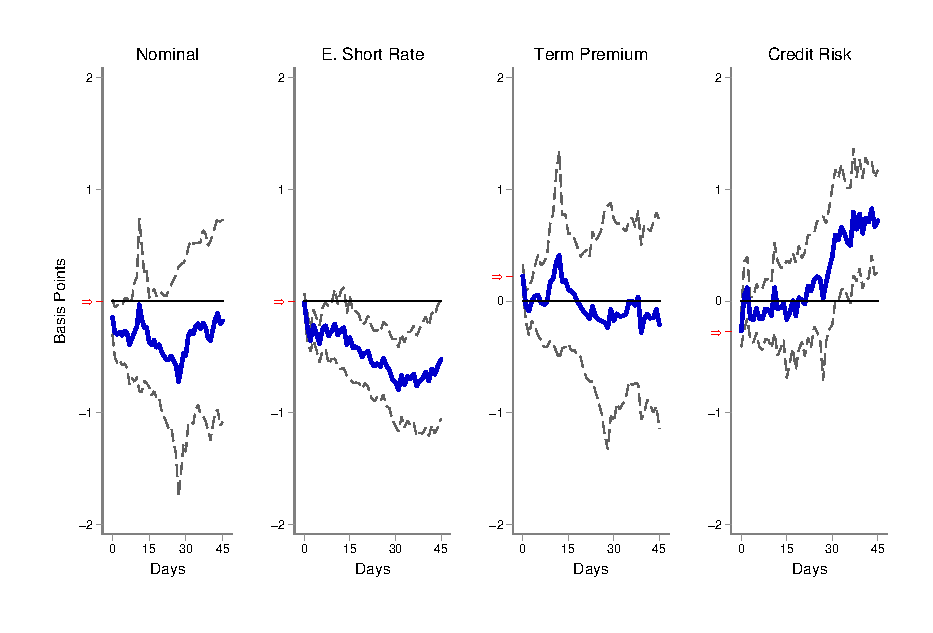
\includegraphics[trim={0cm 0cm 0cm 0cm},clip,height=0.35\textheight,width=\linewidth]{../Figures/LPs/LagDep-FX/Target/EM/TargetEMnomyptpphi120m.eps} \\
						\vspace{-0.35cm}
						\caption{10-Year Yield} \label{subfig:LPEM10Ytarget}
						\vspace{0.4cm}
					\end{subfigure}
				
					\vspace{0.5cm}
					
					\begin{subfigure}[t]{\linewidth}
						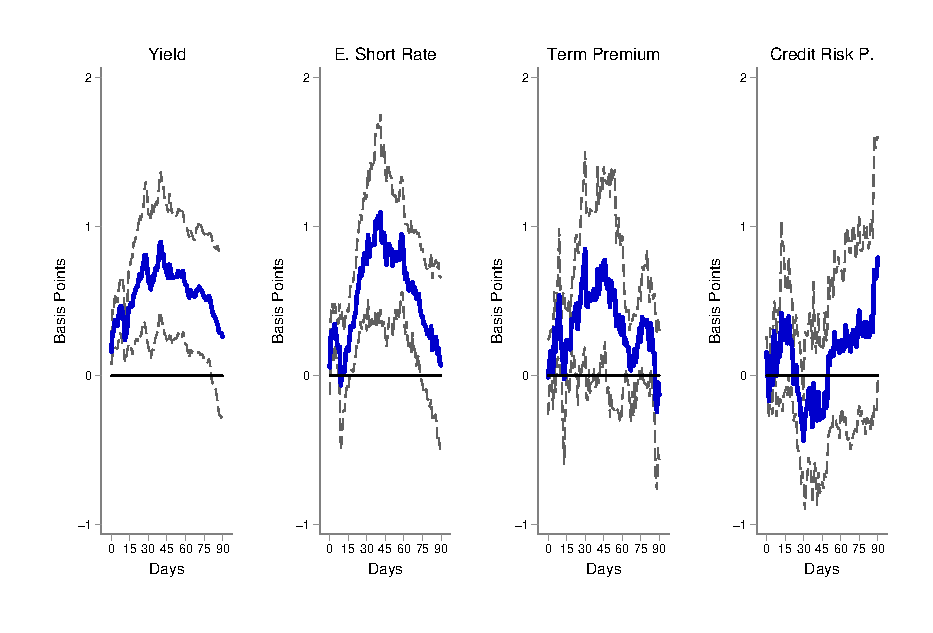
\includegraphics[trim={0cm 0cm 0cm 0cm},clip,height=0.35\textheight,width=\linewidth]{../Figures/LPs/LagDep-FX/Target/EM/TargetEMnomyptpphi24m.eps} \\
						\vspace{-0.35cm}
						\caption{2-Year Yield} \label{subfig:LPEM2Ytarget}
						\vspace{0.4cm}
					\end{subfigure}
				\end{center}
				\fignotes{This figure shows the response following \cite{Jorda:2005} of the 10- and 2-year emerging market nominal yields and their components to a target easing surprise of 1 basis point. Nominal yields are decomposed into an expected future short-term interest rate, a term premium and credit risk compensation, see section \ref{sec:Decomposition} for details. Target surprises are identified using intraday data around Fed's monetary policy announcements, see section \ref{sec:USMPS} for details. An arrow indicates the contemporaneous (\(\idxh = 0\)) effect. The 90\% confidence bands are based on Driscoll--Kraay standard errors.}
			\end{minipage}
		\end{center}
	\end{figure}
	
	\pagebreak[4]
	
	\begin{figure}[tbph]
		\caption{Response of the Yield Curve to a Forward Guidance Surprise: 2000-2008} \label{fig:LPEMpathPre}
		\begin{center}
			\begin{minipage}{\linewidth}
				\begin{center}
					\begin{subfigure}[t]{\linewidth}
						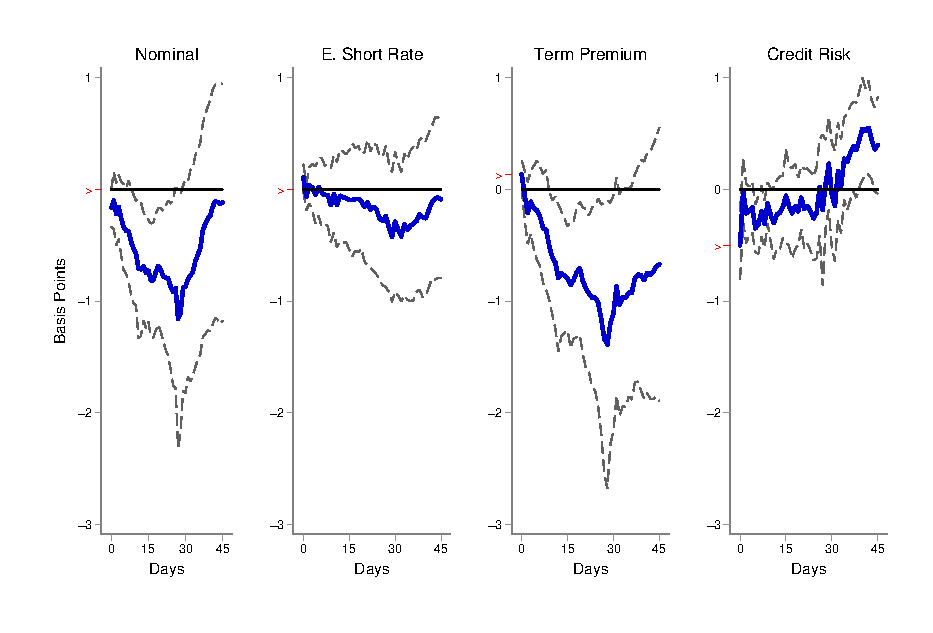
\includegraphics[trim={0cm 0cm 0cm 0cm},clip,height=0.35\textheight,width=\linewidth]{../Figures/LPs/LagDep-FX/Path/EM/PathEMnomyptpphi120mPre.eps} \\
						\vspace{-0.35cm}
						\caption{10-Year Yield} \label{subfig:LPEM10YpathPre}
					\end{subfigure}
					
					\vspace{0.5cm}
					
					\begin{subfigure}[t]{\linewidth}
						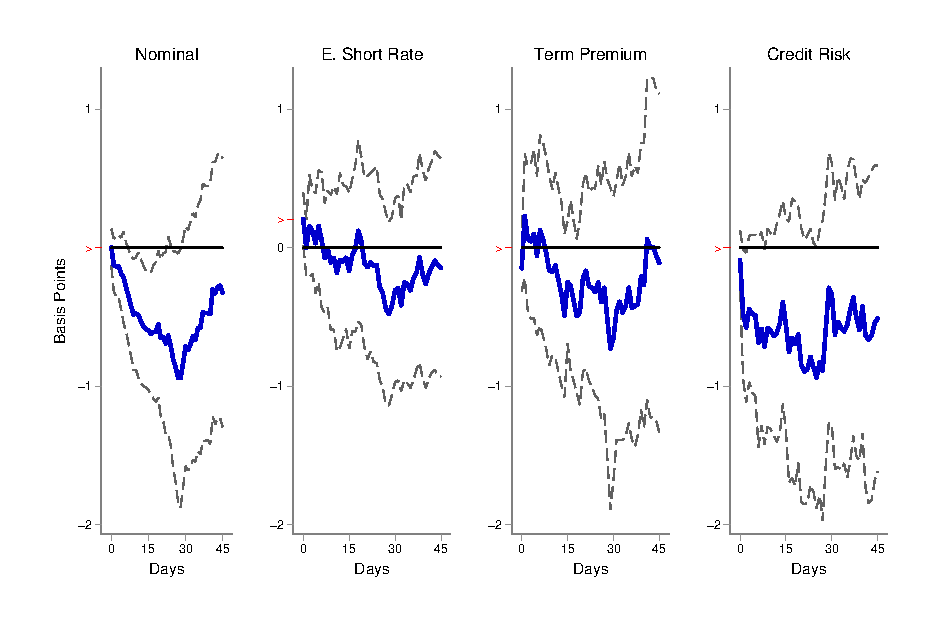
\includegraphics[trim={0cm 0cm 0cm 0cm},clip,height=0.35\textheight,width=\linewidth]{../Figures/LPs/LagDep-FX/Path/EM/PathEMnomyptpphi24mPre.eps} \\
						\vspace{-0.35cm}
						\caption{2-Year Yield} \label{subfig:LPEM2YpathPre}
					\end{subfigure}
				\end{center}
				\fignotes{This figure shows the response following \cite{Jorda:2005} of the 10- and 2-year emerging market nominal yields and their components to a forward guidance easing surprise of 1 basis point. Nominal yields are decomposed into an expected future short-term interest rate, a term premium and credit risk compensation, see section \ref{sec:Decomposition} for details. Forward guidance surprises are identified using intraday data around Fed's monetary policy announcements, see section \ref{sec:USMPS} for details. An arrow indicates the contemporaneous (\(\idxh = 0\)) effect. The 90\% confidence bands are based on Driscoll--Kraay standard errors.}
			\end{minipage}
		\end{center}
	\end{figure}
	
	\pagebreak[4]
	
	\begin{figure}[tbph]
		\caption{Response of the Yield Curve to a Forward Guidance Surprise: 2008-2019} \label{fig:LPEMpathPost}
		\begin{center}
			\begin{minipage}{\linewidth}
				\begin{center}
					\begin{subfigure}[t]{\linewidth}
						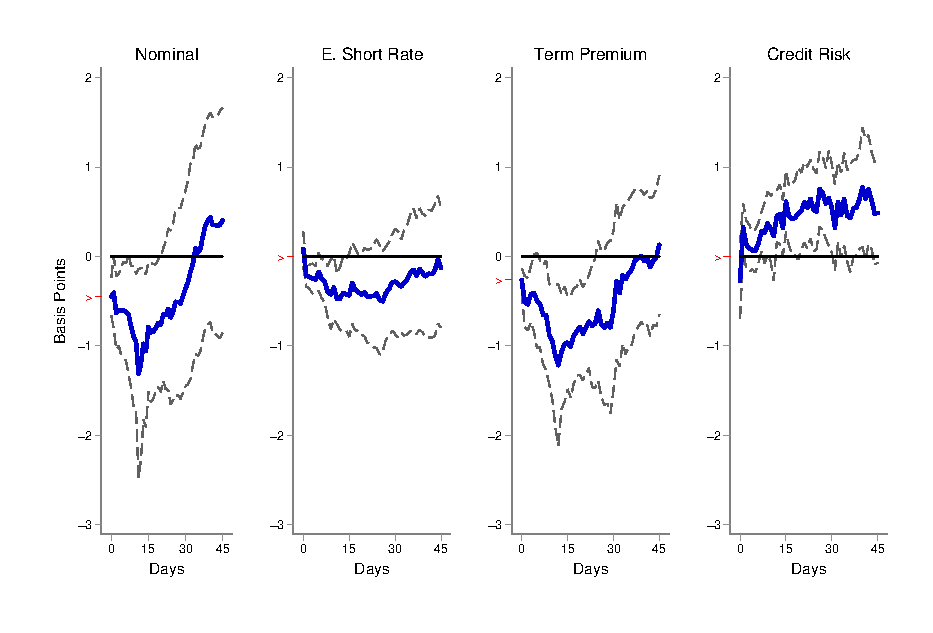
\includegraphics[trim={0cm 0cm 0cm 0cm},clip,height=0.35\textheight,width=\linewidth]{../Figures/LPs/LagDep-FX/Path/EM/PathEMnomyptpphi120mPost.eps} \\
						\vspace{-0.35cm}
						\caption{10-Year Yield} \label{subfig:LPEM10YpathPost}
					\end{subfigure}
					
					\vspace{0.5cm}
					
					\begin{subfigure}[t]{\linewidth}
						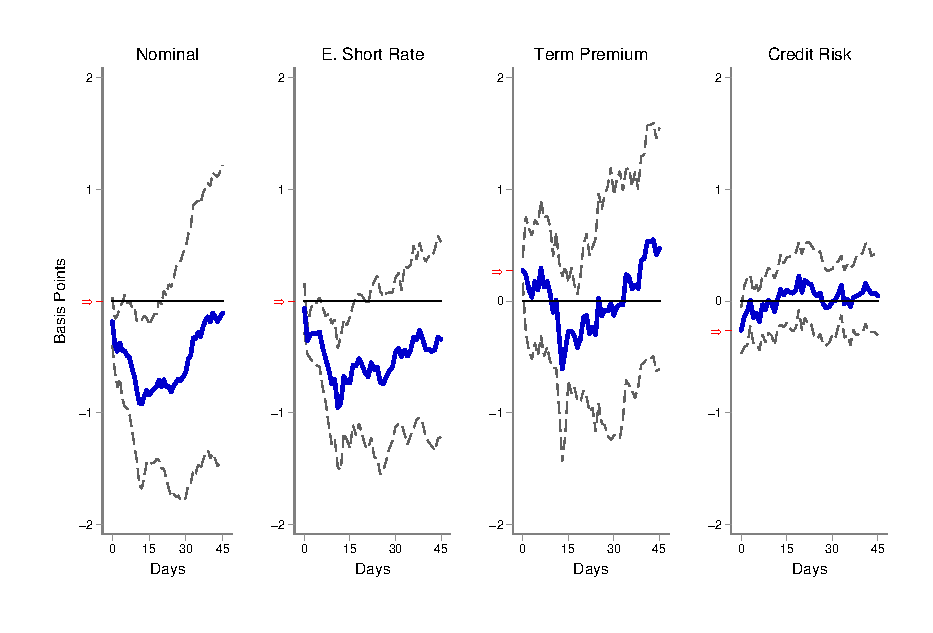
\includegraphics[trim={0cm 0cm 0cm 0cm},clip,height=0.35\textheight,width=\linewidth]{../Figures/LPs/LagDep-FX/Path/EM/PathEMnomyptpphi24mPost.eps} \\
						\vspace{-0.35cm}
						\caption{2-Year Yield} \label{subfig:LPEM2YpathPost}
					\end{subfigure}
				\end{center}
				\fignotes{This figure shows the response following \cite{Jorda:2005} of the 10- and 2-year emerging market nominal yields and their components to a forward guidance easing surprise of 1 basis point. Nominal yields are decomposed into an expected future short-term interest rate, a term premium and credit risk compensation, see section \ref{sec:Decomposition} for details. Forward guidance surprises are identified using intraday data around Fed's monetary policy announcements, see section \ref{sec:USMPS} for details. An arrow indicates the contemporaneous (\(\idxh = 0\)) effect. The 90\% confidence bands are based on Driscoll--Kraay standard errors.}
			\end{minipage}
		\end{center}
	\end{figure}
	
	\pagebreak[4]
	
	\begin{figure}[tbph]
		\caption{Response of the Yield Curve to an Asset Purchase Surprise} \label{fig:LPEMlsap}
		\begin{center}
			\begin{minipage}{\linewidth}
				\begin{center}
					\begin{subfigure}[t]{\linewidth}
						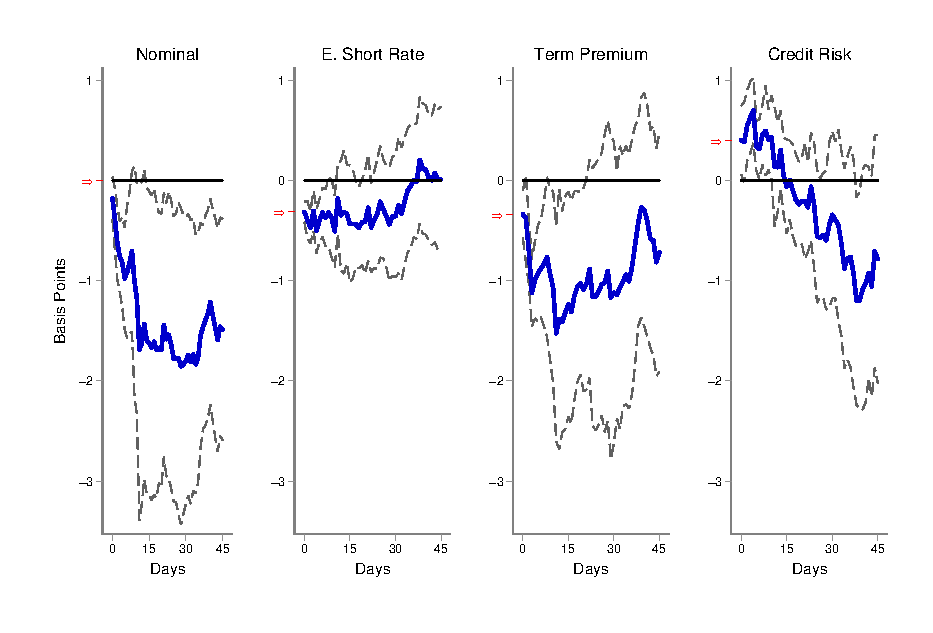
\includegraphics[trim={0cm 0cm 0cm 0cm},clip,height=0.35\textheight,width=\linewidth]{../Figures/LPs/LagDep-FX/LSAP/EM/LSAPEMnomyptpphi120m.eps} \\
						\vspace{-0.35cm}
						\caption{10-Year Yield} \label{subfig:LPEM10Ylsap}
					\end{subfigure}
					
					\vspace{0.5cm}
					
					\begin{subfigure}[t]{\linewidth}
						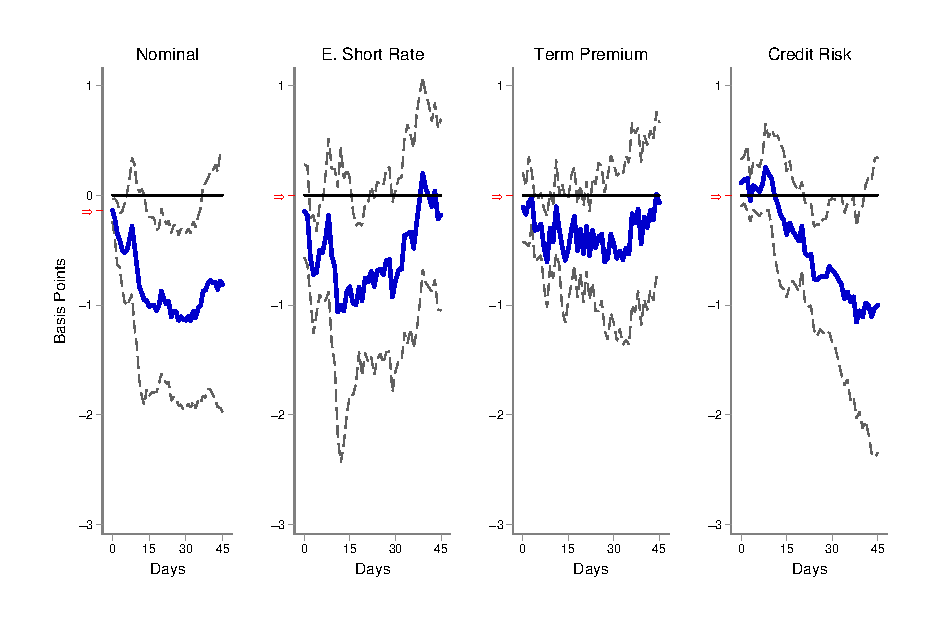
\includegraphics[trim={0cm 0cm 0cm 0cm},clip,height=0.35\textheight,width=\linewidth]{../Figures/LPs/LagDep-FX/LSAP/EM/LSAPEMnomyptpphi24m.eps} \\
						\vspace{-0.35cm}
						\caption{2-Year Yield} \label{subfig:LPEM2Ylsap}
					\end{subfigure}
				\end{center}
				\fignotes{This figure shows the response following \cite{Jorda:2005} of the 10- and 2-year emerging market nominal yields and their components to an asset purchase easing surprise of 1 basis point. Nominal yields are decomposed into an expected future short-term interest rate, a term premium and credit risk compensation, see section \ref{sec:Decomposition} for details. Asset purchase surprises are identified using intraday data around Fed's monetary policy announcements, see section \ref{sec:USMPS} for details. An arrow indicates the contemporaneous (\(\idxh = 0\)) effect. The 90\% confidence bands are based on Driscoll--Kraay standard errors.}
			\end{minipage}
		\end{center}
	\end{figure}
\end{document}
% trim = {<left> <lower> <right> <upper>}

Looking at the effects of a target easing surprise on the yield components in figure \ref{fig:LPEMtarget}, investors expect central banks in emerging markets to follow the monetary stance of the Fed rather than counteract it, as can be seen in the decline of the expected future short rate, particularly at the short end. In fact, most of the effect is reflected on that component; there is essentially no effect on the term premia. 

Notice that the credit risk compensation turns out to be an important factor to understand the transmission of U.S. monetary policy to emerging market yields. 
While there is no effect on the credit risk compensation at the short end, it increases at the long end one month after the surprise. 
Mechanically, both the nominal and synthetic yield curves steepen (since short rates decline) 
but in a way that the long end of the synthetic yield curve declines by more than the nominal one, 
and so borrowing (long-term) directly in LC becomes relatively more expensive. 
Intuitively, loose financial conditions abroad trigger a `reach-for-yield' behavior among investors \citep{HausmanWongswan:2011} that can incentivize more borrowing in emerging markets by sovereigns in local currency \citep{BigioNunoPassadore:2018} and by corporates in foreign currency\footnote{\cite{DuSchreger:2017WP} show that higher reliance on foreign currency borrowing by corporates increases sovereign default risk in emerging markets.}. 
In either case, the price of default risk (not necessarily the risk itself) increases. In line with this, \cite{JeanneretSouissi:2016} conclude that global factors affect investors’ compensation for holding sovereign credit risk, but not the risk itself. 
The effect on the credit risk compensation could be seen as the fiscal implications in emerging markets of Fed's monetary policies, which has so far not been discussed in the literature. 

In sum, economically significant spillovers from target easing surprises build over time reducing the expected future short rate and increasing the long-term credit risk compensation of emerging markets. In this sense, U.S. monetary policy spillovers do not need to involve the term premium.


\subsubsection{Forward Guidance Surprises}
\iftoggle{toclinks}{\gototoc}{} % Turn it on/off in packages.tex, command in macros.tex

Since U.S. monetary policy spillovers to long-term yields increased after the global financial crisis \citep{Albaglietal:2019}, figures \ref{fig:LPEMpathPre} and \ref{fig:LPEMpathPost} display the responses of emerging market yields to a forward guidance easing surprise before and after October 2008, respectively. 
In both cases, the yield responses are sluggish.

Before the global financial crisis, a forward guidance easing surprise led to a downward parallel shift in the yield curves of emerging markets in the month following the surprise. 
The effect on emerging market yields lasted longer than on U.S. yields (cf. figure \ref{fig:LPUSpathPre}), and was generally driven by a decline in all three components. At the long end, it was especially through a decline in the expected short rate and the term premium; these responses are similar to the ones of their U.S. counterparts. These results indicate that investors expected central banks in emerging markets to follow the Fed's monetary stance and that, in line with \cite{Turner:2014}, decisions aimed at reducing the U.S. term premium also reduced the term premia in emerging markets. 

After the global financial crisis, the transmission of forward guidance easing surprises changed. 
The decline in the nominal yields of emerging markets at the long end lasts less than in long-term U.S. yields. 
Therefore, the nominal yield curve in emerging markets steepens relative to the U.S. yield curve in the month following the surprise, so the nominal-synthetic spread in emerging market yields widens at the long end.
The intuition is similar to the one for target surprises above. A loose future path of the U.S. policy rate triggers a `reach-for-yield' behavior among investors and might incentivize more borrowing in emerging markets by sovereigns in local currency and/or by corporates in foreign currency, which increases the price of default risk.

The characterization of the response of the term premia is where accounting for credit risk pays off. 
By signaling a loose future path for the federal funds rate, the Fed attempts to reduce long-term U.S. yields mainly by reducing the term premium (see figure \ref{fig:LPUSpathPost}). 
Figure \ref{fig:LPEMpathPost} shows that the response of the term premia is similar in emerging markets than in the U.S., since forward guidance easing surprises also reduce the term premia in emerging market yields (especially at the long end) which, again, is in line with \cite{Turner:2014}. 
If, instead, credit risk were to be ignored, one would incorrectly conclude that forward guidance does not affect the term premia in emerging markets. The reason is that the `clean' term premium and the credit risk compensation components respond in opposite directions with magnitudes that almost offset each other, so there is no net effect in the term premium contaminated with credit risk.

Notice that a forward guidance easing surprise not only reduces the term premia at the long end 
but also the expectation for the policy rate at the short end, which
supports the risk spillovers mechanism described by \cite{Kalemli-Ozcan:2019}, and is in line with the results reported in section \ref{sec:Drivers}.


\subsubsection{Asset Purchase Surprises}
\iftoggle{toclinks}{\gototoc}{} % Turn it on/off in packages.tex, command in macros.tex

Figure \ref{fig:LPEMlsap} displays the response of emerging market yields to an asset purchase easing surprise. 
Asset purchase surprises not only give rise to a sluggish in responses in the yields, as target and forward guidance surprises do, but their effects last longer in emerging market yields than in U.S. yields. This result suggests that portfolio rebalancing involving emerging market bonds following asset purchases is slower.

An asset purchase easing surprise also flattens the yield curve in emerging markets, similar to the effect on the U.S. yield curve (see figure \ref{fig:LPUSlsap}). 
In both cases, the effect at the long end is larger than at the short end over time. 
The on-impact response of U.S. yields is larger, whereas the response of the nominal yields of emerging markets lasts longer, as already mentioned. 
These two effects in turn explain the response of the credit risk compensation at the long end, which initially increases followed by a sluggish and considerable decline. 
The counterintuitive initial increase is more a reflection of the response in the U.S. Treasuries market than on the bond markets in emerging economies. 
Indeed, an asset purchase easing surprise triggers a strong investor reaction in the U.S. Treasuries market, leading to a  more than one-to-one on-impact decline in the long-term U.S. yield (see figure \ref{subfig:LPUS10Ylsap}).

Notice that the eventual decline in the credit risk compensation as well as the reduction in the term premium reflect a relaxation of global financial conditions; investors' more willingness to buy the long-term debt of emerging markets, reduces those countries' borrowing costs. 

Finally, similar to the effects of a forward guidance easing surprise after 2008, an asset purchase easing surprise reduces the term premia at the long end and the expectation for the policy rate at the short end, also in line with the risk spillovers mechanism in \cite{Kalemli-Ozcan:2019}.

}{}	% Closes \iftoggle{fulldraft}


\section{Concluding Remarks} \label{sec:conclusions}
\iftoggle{toclinks}{\gototoc}{} % Turn it on/off in packages.tex, command in macros.tex
\iftoggle{cboxes}{	   				  % Turn it on/off in packages.tex
	\begin{boxeditems}
		\item None.
	\end{boxeditems}}{}

This paper decomposes the sovereign yields of 15 emerging markets taking into account the credit risk embedded in them, and empirically quantifies the transmission channels of U.S. monetary policy to them.  Emerging market nominal yields are decomposed into average expected future short rates, a term premium and compensation for credit risk. 

\iftoggle{fulldraft}{					% Turn it on/off in packages.tex

The responses of emerging market yields to target, forward guidance and asset purchase surprises are sluggish, and amplify over time. 
Moreover, U.S. monetary policy transmits to emerging market yields through their different components, what can be referred to as the yield curve channel. 
The yield decompositions show that surprises in Fed's policy decisions lead to a reassessment of policy rate expectations and a repricing of interest rate risk as well as of credit risk in emerging markets. 
Specifically, investors expect monetary authorities in emerging markets to follow the Fed's monetary stance rather than counteract it; the response of the term premia in emerging markets is similar to that of the U.S. term premium; and Fed's monetary policy decisions also affect investors’ compensation for holding emerging markets' sovereign credit risk, consistent with a `reach-for-yield' behavior among investors. 
The effect on credit risk has not been explored before and it is a prospective area for future research.

Overall, the results show that to adequately characterize the transmission channels of U.S. monetary policy, it is important to explicitly account for credit risk in the local currency debt of emerging markets and to examine the effects at different maturities.

The results presented here can be extended in several directions.
The proposed three-part decomposition of emerging market yields has many applications, such as analyzing the transmission of monetary policy domestically and further decomposing each part (e.g., average expected short rates can be split into inflation and real interest rate expectations).
The results might also inform theoretical models for pricing sovereign defaultable bonds. 
Finally, surprises from other central banks in advanced economies could be included in the analysis of monetary policy spillovers to see whether they also influence the yields of emerging markets and, if so, how their influence differs from that of the Fed. 

}{}	% Closes \iftoggle{fulldraft}


\bibliographystyle{abbrvnat} 	% Other styles: {plain}, {authordate1}

% Local copy of the database with references
% Might need to run file_duplicator.sh first
% To clean removed references, in the terminal execute
% $ cd Book/Ch_Synthetic/Docs/Paper
% $ bibexport -o ../References/library.bib paper.aux
%\bibliography{../References/library}

% Centralized database with references
% It does not need executing file_duplicator.sh
% Con: it might show removed citations that were previously included
\bibliography{../../../References/library}

\newpage
\begin{appendices}
\iftoggle{toclinks}{\gototoc}{} % Turn it on/off in packages.tex, command in macros.tex
\iftoggle{cboxes}{	   				  % Turn it on/off in packages.tex
	\begin{boxeditems}
		\item Add link to website for Excel file with tickers.
		\item Add reference to paper that compares YC from Bloomberg for the Euro area.
	\end{boxeditems}}{}


\section{Trend Inflation as a Proxy for Long-Term Inflation Forecasts} \label{sec:trendinf}

An advantage of the small open economy approach is that it only requires forecasts for inflation, or a proxy in the case of countries with no long-term forecasts available as is the case for Israel and South Africa.
Inflation expectations are hoped to match measures of inflation that exclude unexpected shocks and better reflect the inflation environment.
Different measures of core inflation exist.
I use the inflation trend obtained by applying the Hodrick-Prescott filter to the series of realized inflation of each country.
Of course, the filter is sensitive to the sample period used.
The resulting trend can also be outside of the target inflation band due to the innate dynamics of the series, which would be at odds with survey data (see figure \ref{fig:wnCPI}).
Fortunately, unlike other countries, there is no marked upward or downward trend in the inflation of the two countries during the sample period.
For each country, trend inflation is calculated for the whole period but only considered within the time range for which survey data is available for the rest of the countries, and as long as the trend is within the inflation target band.
Figure \ref{fig:CPI_ILSZAR} shows the realized and trend inflation for Israel and South Africa, and compares them with those of Malaysia and Thailand, two countries with a similar pattern for inflation (i.e. no marked trend) and for which survey data is available.
%It supports that t
Trend inflation seems to be a good proxy for the long-term inflation forecasts of Israel and South Africa.
Finally, since the 5-year and long-term forecasts closely follow each other (see figure \ref{fig:wnCPI}), I use trend inflation for both tenors.

\begin{landscape}
	\documentclass{article}
\usepackage{graphicx}
\usepackage[margin=1in]{geometry}
\usepackage[outdir=./]{epstopdf}  					% Avoids errors when input figures
\usepackage[labelsep=period,labelfont=bf]{caption}
%\usepackage{subcaption}

\begin{document}
	\begin{figure}[tbph]
		\caption{Inflation Trend and Long-Horizon Forecast for Inflation} \label{fig:CPI_ILSZAR}
		\begin{center}								% center the minipage on the line
			\begin{minipage}{0.9\linewidth}
				\begin{center}							% center the figure inside the minipage
					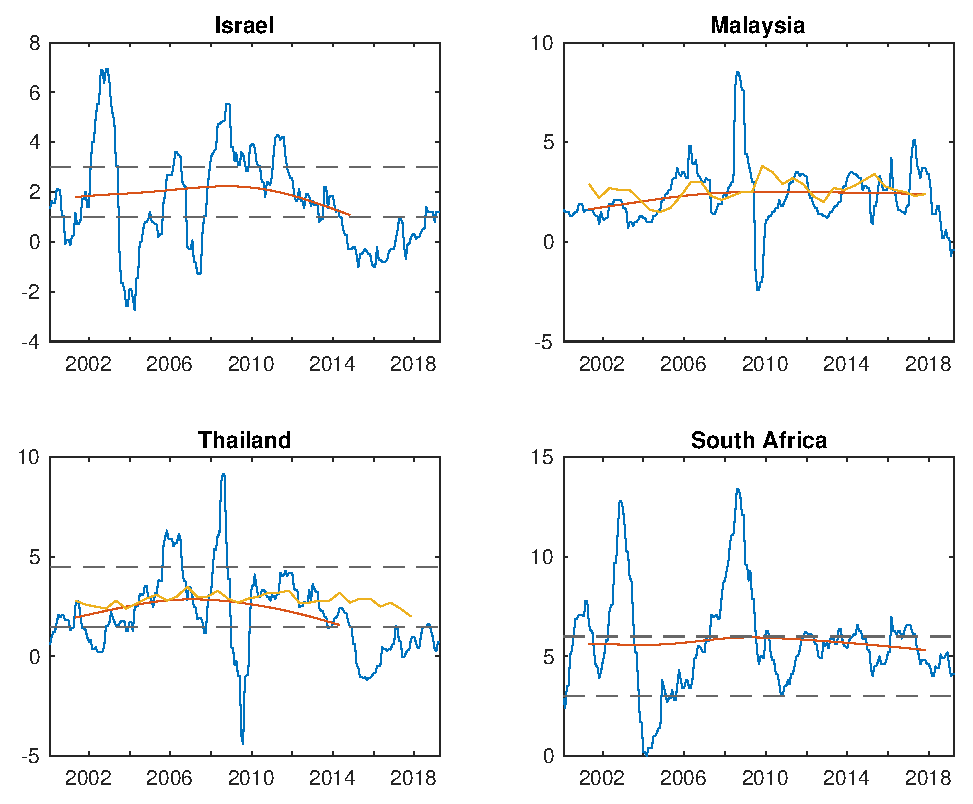
\includegraphics[trim={0cm 0cm 0cm 0cm},clip,height=0.85\textheight,width=1\textwidth]{../Figures/Surveys/CPI_ILSZAR.eps} \\
				\end{center}
				\fignotes{This figure plots consumer price inflation (solid line), inflation trend based on the Hodrick--Prescott filter (dash-dotted line) and long-term inflation forecast (dashed line). The figure also includes the upper and lower bounds for the domestic inflation target. The upper and lower bounds are the most recent ones for each country.}
			\end{minipage}
		\end{center}
	\end{figure}
\end{document}
% trim = {<left> <lower> <right> <upper>}
\end{landscape}

%		\begin{figure}[!htbp]
		\begin{centering}
			\vspace{12.5mm}
			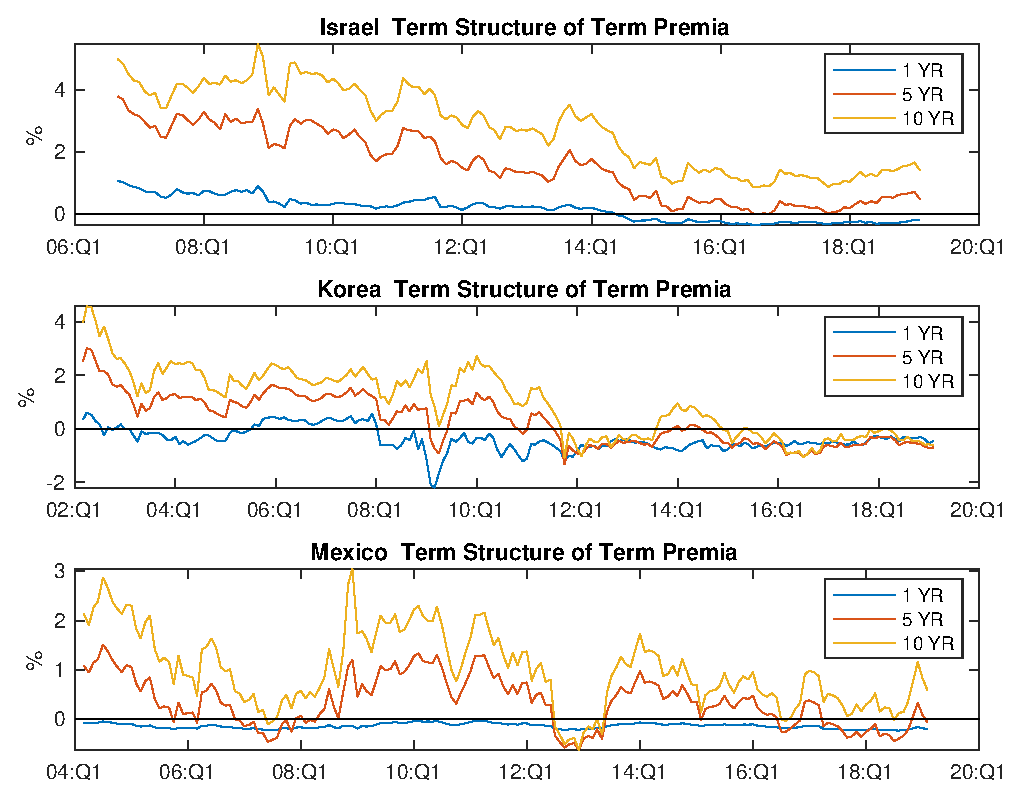
\includegraphics[width=1\textwidth,height=0.8\textheight]{../Figures/Temp/temp_ts_tp}
			\par\end{centering}
		\caption{Estimated Term Premia for Different Maturities.}\label{fig:temp_ts_tp}
	\end{figure}

%\newgeometry{top=4cm, left=5.5cm}	% Modify this if more space is needed
%%\newgeometry{margin=1cm}  % To make the table fit your landscape
%\begin{landscape}
%	\begin{table}
\centering
\begin{tabular}{l|cccccccccccccc}
\toprule
&\textbf{COP}&\textbf{HUF}&\textbf{IDR}&\textbf{ILS}&\textbf{MXN}&\textbf{PEN}&\textbf{PHP}&\textbf{PLN}&\textbf{TRY}&\textbf{KRW}&\textbf{MYR}&\textbf{RUB}&\textbf{THB}&\textbf{ZAR}\\\midrule
{ Coeff.}&1.17&-0.28&-0.32&1.02&0.42&1.50&-0.14&0.43&1.41&1.02&-0.23&1.37&0.82&-0.35\\\
{S.E.}&0.24&0.15&0.20&0.11&0.15&0.32&0.24&0.11&0.27&0.12&0.10&0.40&0.17&0.21\\\
{pVal}&0.00&0.07&0.10&0.00&0.01&0.00&0.55&0.00&0.00&0.00&0.02&0.00&0.00&0.10\\\
{Obs}&154&138&205&146&173&141&219&157&155&219&136&144&137&218\\\
{$R^2$}&0.13&0.02&0.01&0.37&0.04&0.13&0.00&0.10&0.16&0.26&0.04&0.08&0.15&0.01\\ \bottomrule
\end{tabular}
\\
\caption{Regression of 5-Year Risk Premium on $\ln (VIX)$.}\label{tab:rp_reg_lvix}
\end{table}
%\end{landscape}
%\restoregeometry

\end{appendices}

\newpage
\iftoggle{commentboxes}{\maketoc}	% Defined in packages.tex and macros.tex

%\listoftodos
\end{document}

% Source for cleaning .bib file from removed citations https://tex.stackexchange.com/questions/41821/creating-bib-file-containing-only-the-cited-references-of-a-bigger-bib-file